%%%%%%%%%%%%%%%%%%%%%%%%%%%%%%%%%%%%%%%%%
% Journal Article
% LaTeX Template
% Version 1.3 (9/9/13)
%
% This template has been downloaded from:
% http://www.LaTeXTemplates.com
%
% Original author:
% Frits Wenneker (http://www.howtotex.com)
%
% License:
% CC BY-NC-SA 3.0 (http://creativecommons.org/licenses/by-nc-sa/3.0/)
%
%TODO: references and bibliography, theory section, CJ section, intro
% Which SRC values to use? I used original a2 predicted values...
%
%
%
%
%%%%%%%%%%%%%%%%%%%%%%%%%%%%%%%%%%%%%%%%%

%----------------------------------------------------------------------------------------
%	PACKAGES AND OTHER DOCUMENT CONFIGURATIONS
%----------------------------------------------------------------------------------------

\documentclass[oneside]{article}

\usepackage{lipsum} % Package to generate dummy text throughout this template
\usepackage{amsmath}
\usepackage[sc]{mathpazo} % Use the Palatino font
\usepackage[T1]{fontenc} % Use 8-bit encoding that has 256 glyphs
\linespread{1.05} % Line spacing - Palatino needs more space between lines
\usepackage{microtype} % Slightly tweak font spacing for aesthetics
\usepackage{amsmath}

\usepackage[hmarginratio=1:1,top=32mm,columnsep=20pt]{geometry} % Document margins
\usepackage{multicol} % Used for the two-column layout of the document
\usepackage[hang, small,labelfont=bf,up,textfont=it,up]{caption} % Custom captions under/above floats in tables or figures
\usepackage{booktabs} % Horizontal rules in tables
\usepackage{float} % Required for tables and figures in the multi-column environment - they need to be placed in specific locations with the [H] (e.g. \begin{table}[H])
\usepackage{hyperref} % For hyperlinks in the PDF
\restylefloat{figure}
\usepackage{graphicx}
\usepackage{array}
\newcolumntype{C}[1]{>{\centering\arraybackslash}p{#1}}

\usepackage{lettrine} % The lettrine is the first enlarged letter at the beginning of the text
\usepackage{paralist} % Used for the compactitem environment which makes bullet points with less space between them

\usepackage{abstract} % Allows abstract customization
\renewcommand{\abstractnamefont}{\normalfont\bfseries} % Set the "Abstract" text to bold
%\renewcommand{\abstracttextfont}{\normalfont\small\itshape} % Set the abstract itself to small italic text

\usepackage{titlesec} % Allows customization of titles
%\renewcommand\thesection{\Roman{section}} % Roman numerals for the sections
%\renewcommand\thesubsection{\Roman{subsection}} % Roman numerals for subsections
%\titleformat{\section}[block]{\large\scshape\centering}{\thesection.}{1em}{} % Change the look of the section titles
\titleformat{\subsection}[block]{\large}{\thesubsection.}{1em}{} % Change the look of the section titles

\usepackage{fancyhdr} % Headers and footers
\pagestyle{fancy} % All pages have headers and footers
\fancyhead{} % Blank out the default header
\fancyfoot{} % Blank out the default footer
%\fancyhead[C]{Hall C Collaboration $\bullet$ \today} % Custom header text
\fancyhead[C]{\today} % Custom header text
\fancyfoot[RO,LE]{\thepage} % Custom footer text
\usepackage{authblk}

%----------------------------------------------------------------------------------------
%	TITLE SECTION
%----------------------------------------------------------------------------------------

\title{\vspace{-15mm}\fontsize{20pt}{10pt}\selectfont\textbf{A new method to study the EMC Effect using the $F_2^{n}$ structure function}} % Article title

\author[1]{H. Szumila-Vance}
\author[2]{I. Cloet}
\author[1]{C. Keppel}
\author[3]{S. Escalante}
\author[3]{N. Kalantarians}
\affil[1]{Thomas Jefferson National Accelerator Facility, Newport News, VA}
\affil[2]{Argonne National Laboratory, Argonne, IL}
\affil[3]{Virginia Union University, Richmond, VA}
\renewcommand\Authands{ , }



%\author{
%\large
%\textsc{Holly Szumila-Vance}\thanks{}\\[2mm] % Your name
%\normalsize Jefferson Lab \\ % Your institution
%\normalsize \href{mailto:hszumila@jlab.org}{hszumila@jlab.org} % Your email address
%\vspace{-5mm}
%}
\date{}

%----------------------------------------------------------------------------------------

\begin{document}

\maketitle % Insert title

\thispagestyle{fancy} % All pages have headers and footers

%----------------------------------------------------------------------------------------
%	ABSTRACT
%----------------------------------------------------------------------------------------

\begin{abstract}
The persistently mysterious deviations from unity of the ratio of nuclear target structure functions to those of deuterium as measured in deep inelastic scattering (termed the ``EMC Effect") have become the canonical observable for studies of nuclear medium modifications to free nucleon structure in the valence regime. The structure function of the free proton is well known from numerous experiments spanning decades. The free neutron structure function, however, has remained difficult to access. Only recently has it been extracted in a systematic study of the global data within a parton distribution function extraction framework and is available from the CTEQ-Jefferson Lab (CJ) Collaboration. Here we leverage the latter to introduce a new method to study the EMC Effect in nuclei by re-examining existing data and by now determining the magnitude of the medium modifications to the free neutron and proton structure functions independently. From the extraction of the free neutron from world data, it is possible to examine the nuclear effects in deuterium and their contribution to our interpretation of the EMC Effect. In this study, we observe that the ratio of the deuteron to the sum of the free neutron and proton structure functions has some $x_{B}$ and $Q^{2}$ dependencies implying that the magnitude of the standard EMC Effect is in part due to the nuclear effects of the deuteron and also exhibits some $x_{B}$ and $Q^{2}$ dependence.
\end{abstract}
%\newpage
%\tableofcontents
%\newpage
 %\listoffigures
% \newpage
%\listoftables
%\newpage
%----------------------------------------------------------------------------------------
%	ARTICLE CONTENTS
%----------------------------------------------------------------------------------------


\section{Introduction}

Deep inelastic scattering experiments 

\begin{figure}[H]
  \centering
      	  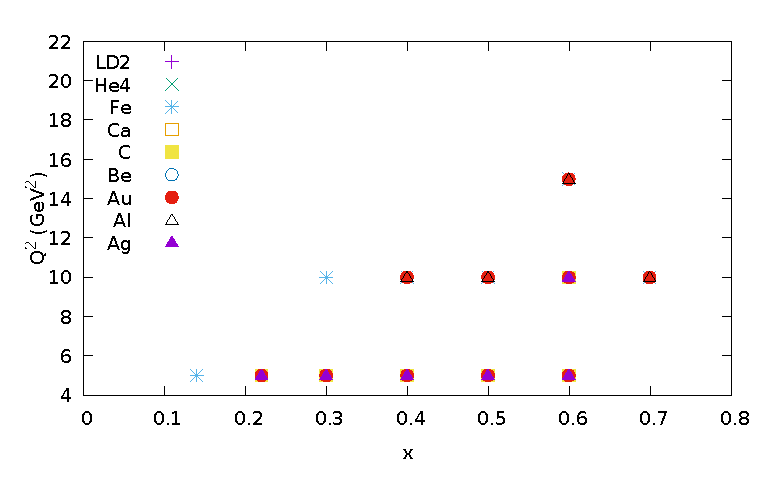
\includegraphics[width=0.5\textwidth]{plots/F2ADdataQ2vsx.eps}
 	 \caption[]{}
  \label{fig:slac_q2x}
 \end{figure} 
 
\section{Theory predictions using nuclear matter}

Discussion points: predicted d/n and d/p ratios, interpretations in quark distributions, emc effects in deuterium


  
\begin{figure}[H]
  \centering
      	  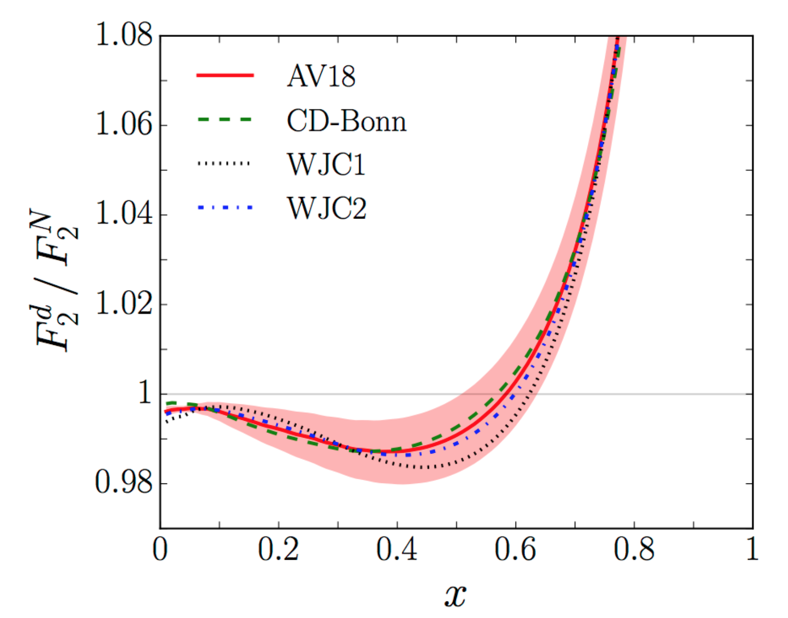
\includegraphics[width=0.5\textwidth]{plots/dn_effects_theory.png}
 	 \caption[Theoretical extraction of the ratio of $F_2^d/F_2^N$]{The theoretical extraction of the ratio of $F_2^d/F_2^N$. The deuteron exhibits some $x_B$-dependence such that the ratio is modified by approximately 2$\%$ in the regime of $x_B$ between 0.3--0.7 (region of interest to the EMC Effect).}
  \label{fig:dn_theory}
 \end{figure}  
 
\begin{figure}[H]
  \centering
      	  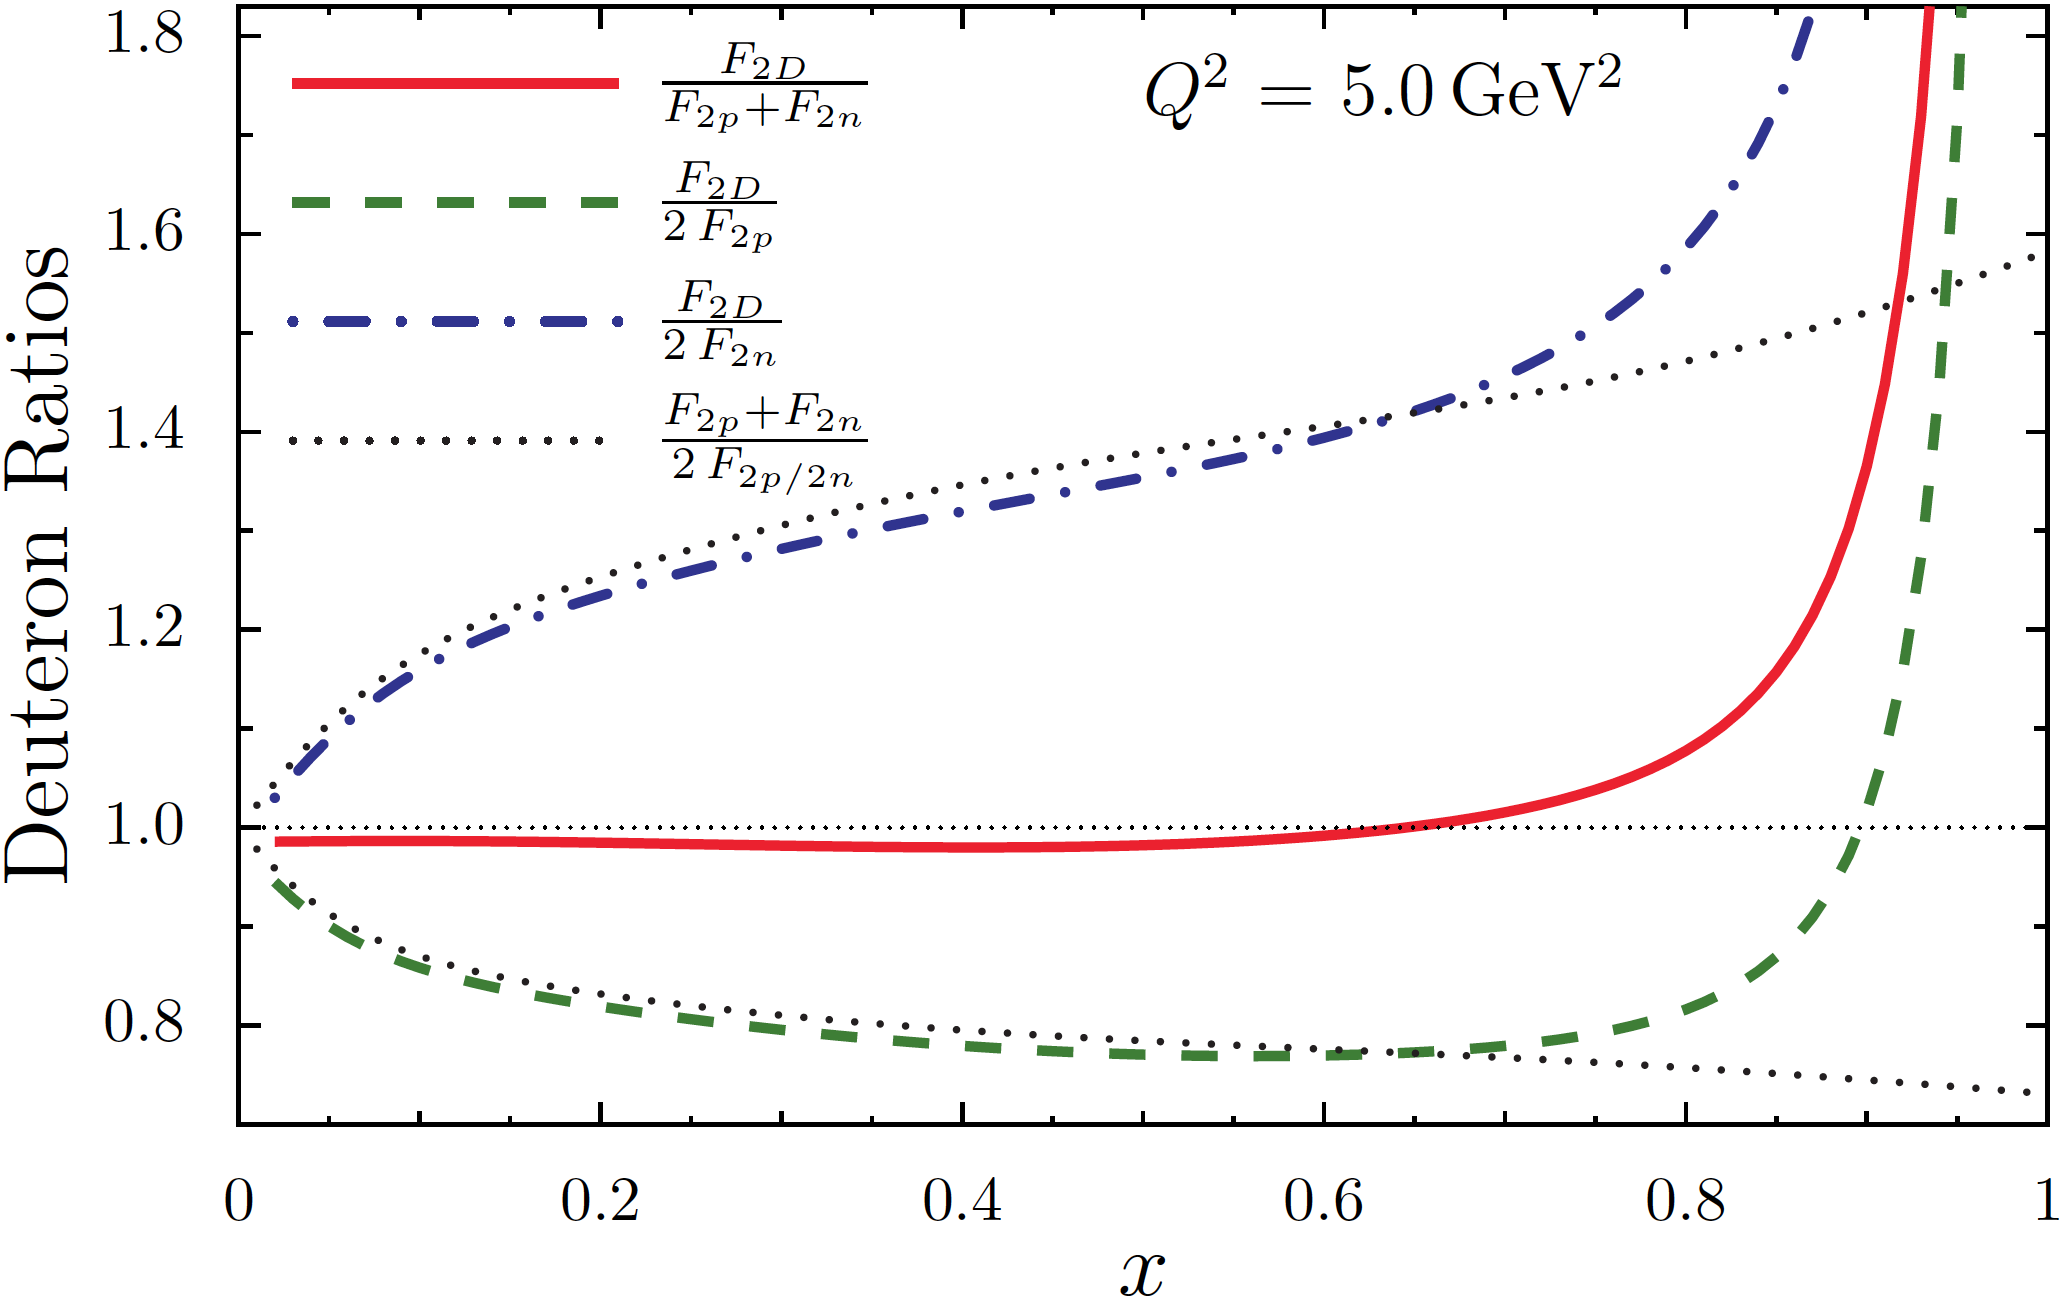
\includegraphics[width=0.5\textwidth]{plots/deut_ratio_theory.png}
 	 \caption[Theoretically-derived deuteron $F_2$ ratios with respect to the free nucleons]{Theoretically-derived deuteron $F_2$ ratios with respect to the free neutron and proton, the free proton, and the free neutron are shown for $Q^2=5$ GeV$^2$.}
  \label{fig:deut_theory}
 \end{figure}  
  
\section{$F_2^n$ extraction and the CJ15 fit}

Recent work by the CTEQ-Jefferson Lab (CJ) Collaboration reviewed the world DIS data on the proton and deuteron structure functions and extracted the free neutron structure function over the full range of kinematics. Through the application of the latest and best known deuteron nuclear corrections, the full global DIS data set provides the equivalent neutron data set. This extracted free neutron structure function enables the authors of this paper to examine the EMC Effect in a new way. 

In Fig.~\ref{fig:F2np_general}, general comparisons of the newly extract $F_2^n$ are made with respect to the $F_2^p$ as derived by the NMC fit. 

 \begin{figure}
\begin{minipage}{0.5\textwidth}
 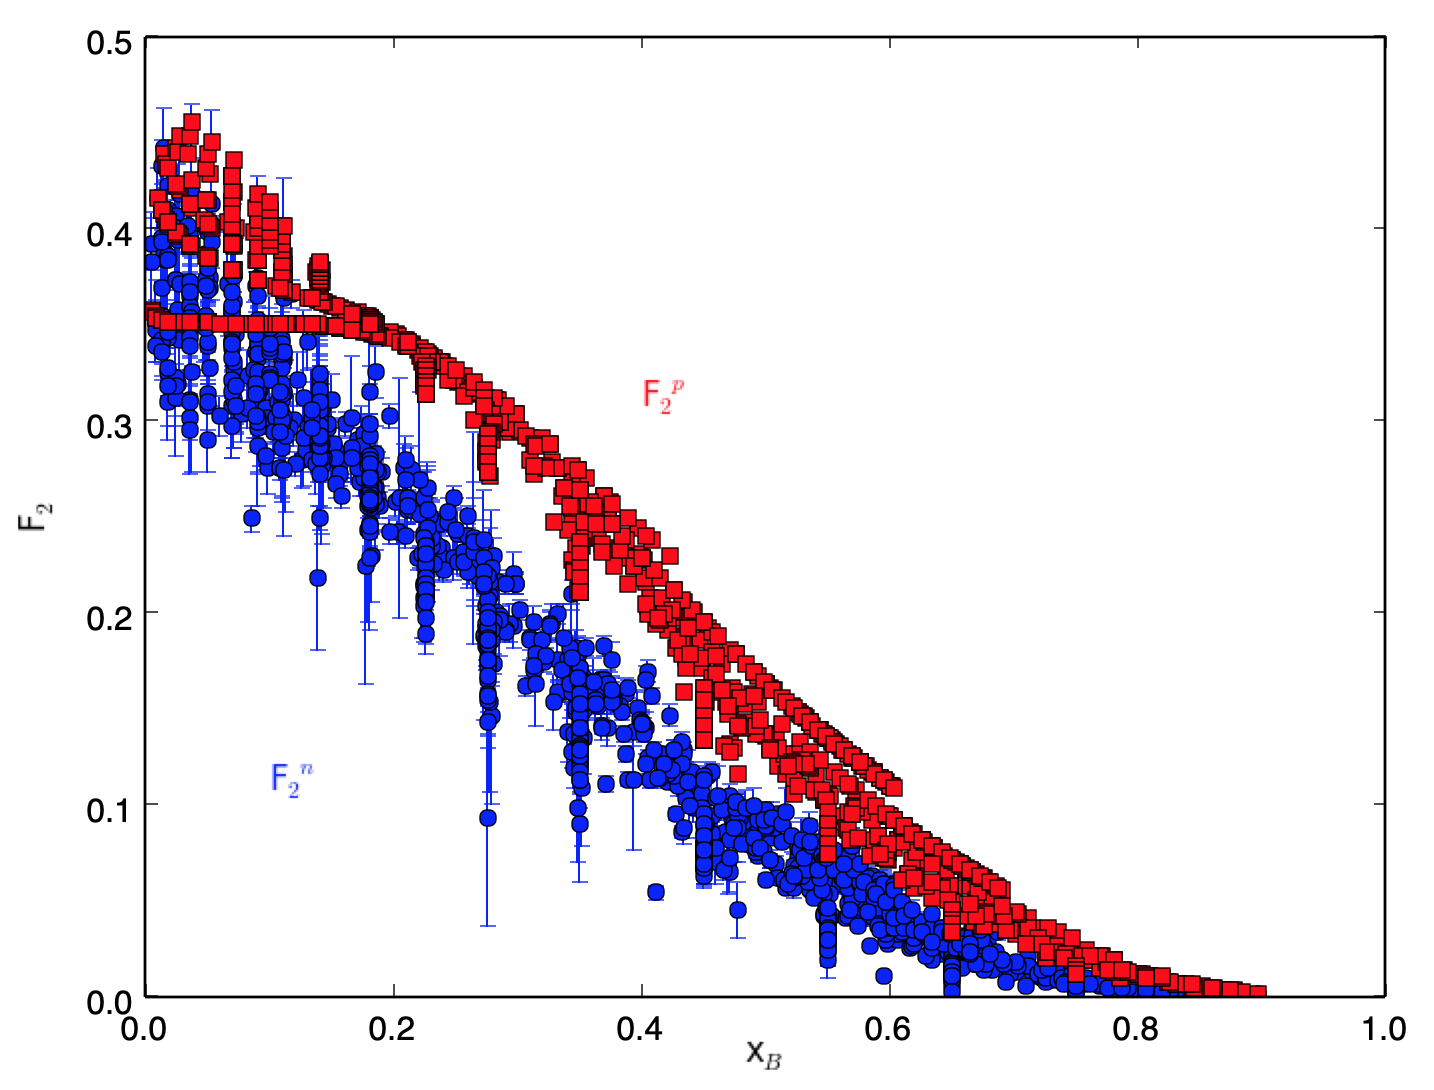
\includegraphics[width=\textwidth]{plots/f2np_plot.png}
\end{minipage}\hfill\begin{minipage}{0.5\textwidth}
 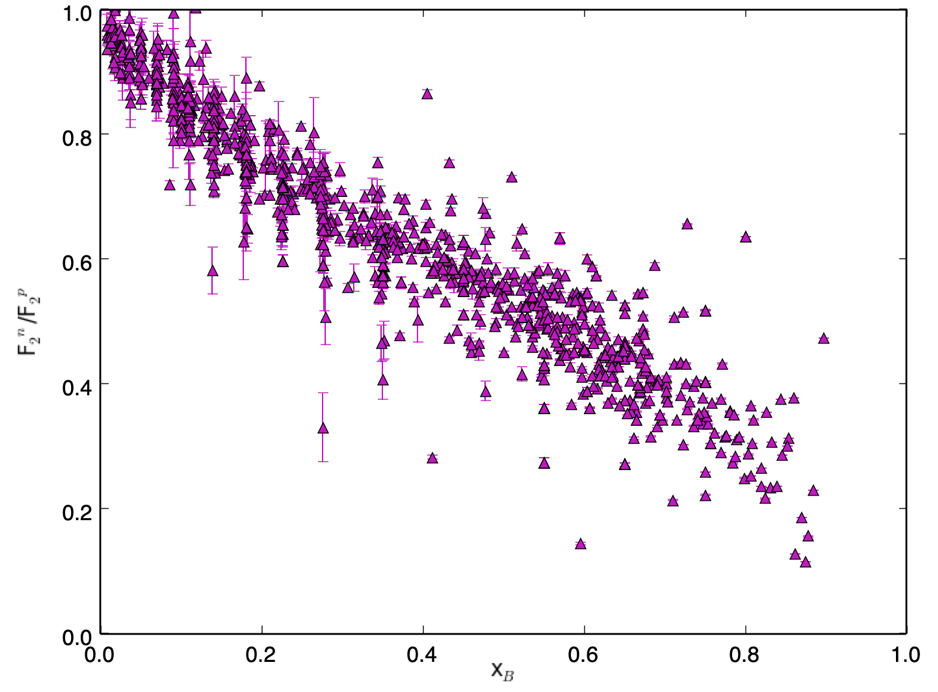
\includegraphics[width=\textwidth]{plots/f2npratio_plot.png}
 \end{minipage}
  \caption[$F_2^{n,p}$ characteristics]{Left: The extracted $F_2^n$ from the world DIS data is shown in blue, and the $F_2^p$ from the NMC global fit is shown in red for the same corresponding $x_B$ and $Q^2$. Right: The ratio of the $F_2^n/F_2^p$ from the left is shown as a function of $x_B$.}
  \label{fig:F2np_general}
\end{figure} 

On the left of Fig.~\ref{fig:F2np_general}, the $F_2^n$ and $F_2^p$ for the same $x_B$ and $Q^2$ kinematics is shown. The $F_2^n$ in blue is the extracted points from the world data, and the $F_2^p$ is the corresponding value (for the same kinematics) from the NMC fit. The overall $x_B$ dependence is somewhat different as the neutron structure function is more comparable at larger $x_B$ while the proton structure function drops off more sharply. The ratio of these quantities is shown on the right in Fig.~\ref{fig:F2np_general} and agrees with previously extracted results. %%%%Insert references here!!
 
\subsection{$Q^2$ dependence}

A significant observation in the CJ15-extracted structure functions is the $Q^2$ dependence. The proton structure function is shown on the left in Fig.~\ref{fig:pd_CJ15} for various $Q^2$ from the CJ15 fit to the world DIS data. The corresponding deuteron structure function is shown on the right in Fig.~\ref{fig:pd_CJ15}. The SLAC E139 experiment took measurements at $Q^2$ in the range of 5--15 GeV$^2$. The proton and deuteron structure functions both show clear differences for the same values of $x_B$ over this range of $Q^2$. 

\begin{figure}
\begin{minipage}{0.5\textwidth}
 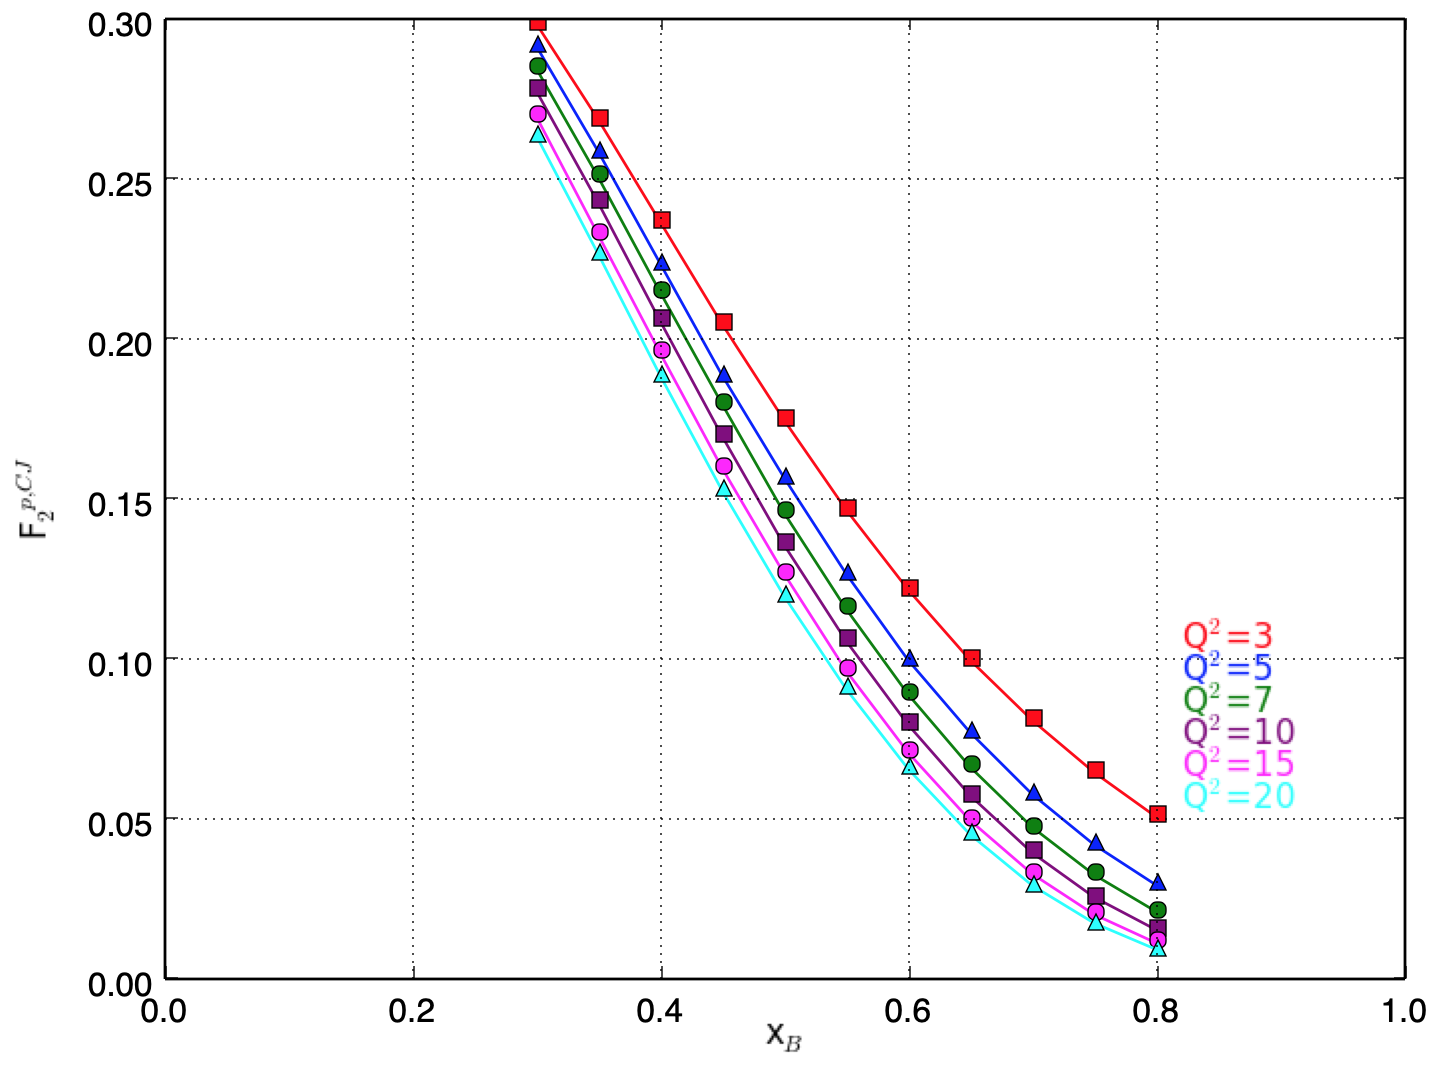
\includegraphics[width=\textwidth]{plots/p_CJ.png}
\end{minipage}\hfill\begin{minipage}{0.5\textwidth}
 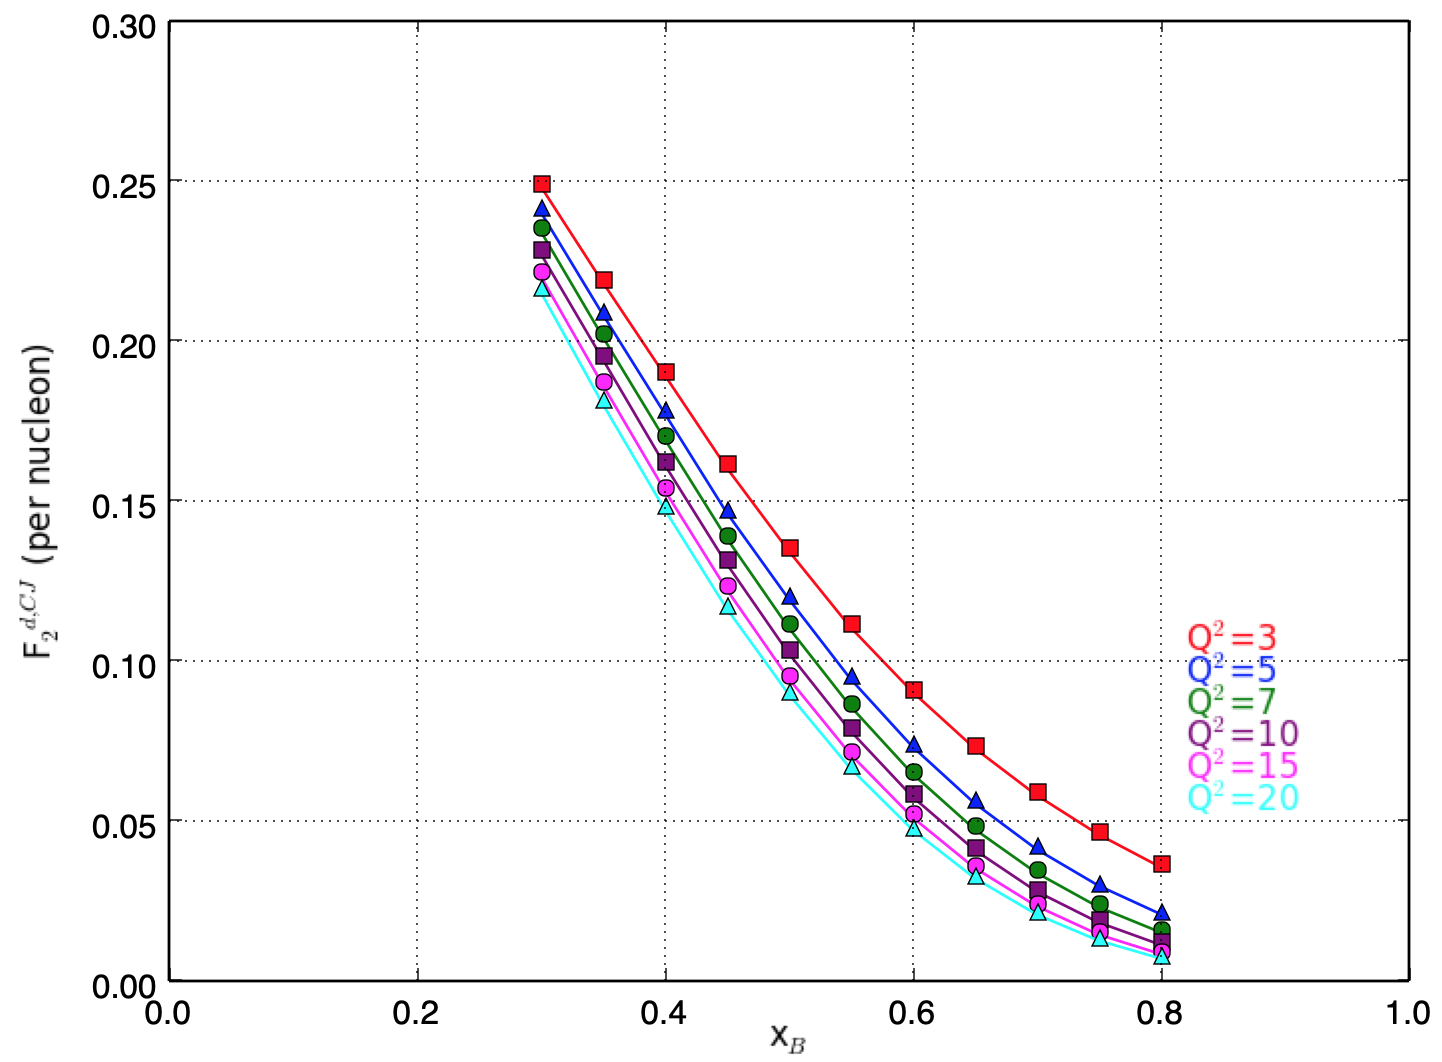
\includegraphics[width=\textwidth]{plots/d_CJ.png}
 \end{minipage}
  \caption[Proton and deuteron from CJ15]{Left: The proton structure function from the CJ15 fit is shown as a function of $x_B$ for various fixed $Q^2$. Right: The deuteron structure function from the CJ15 fit is shown as a function of $x_B$ for various fixed $Q^2$.}
  \label{fig:pd_CJ15}
\end{figure} 
 
The nuclear effects of the proton and neutron in the deuteron can be directly characterized by dividing the deuteron structure function by the sum of the free proton and free neutron structure functions. The result is shown on the left in Fig.~\ref{fig:dpn_cj}. Over the typical range of $x_B$ that is relevant to the EMC Effect, the $Q^2$ dependence is minimal. At approximately $x_B=0.6$ and greater, the ratio varies greatly with $Q^2$.  
 
 \begin{figure}
\begin{minipage}{0.5\textwidth}
 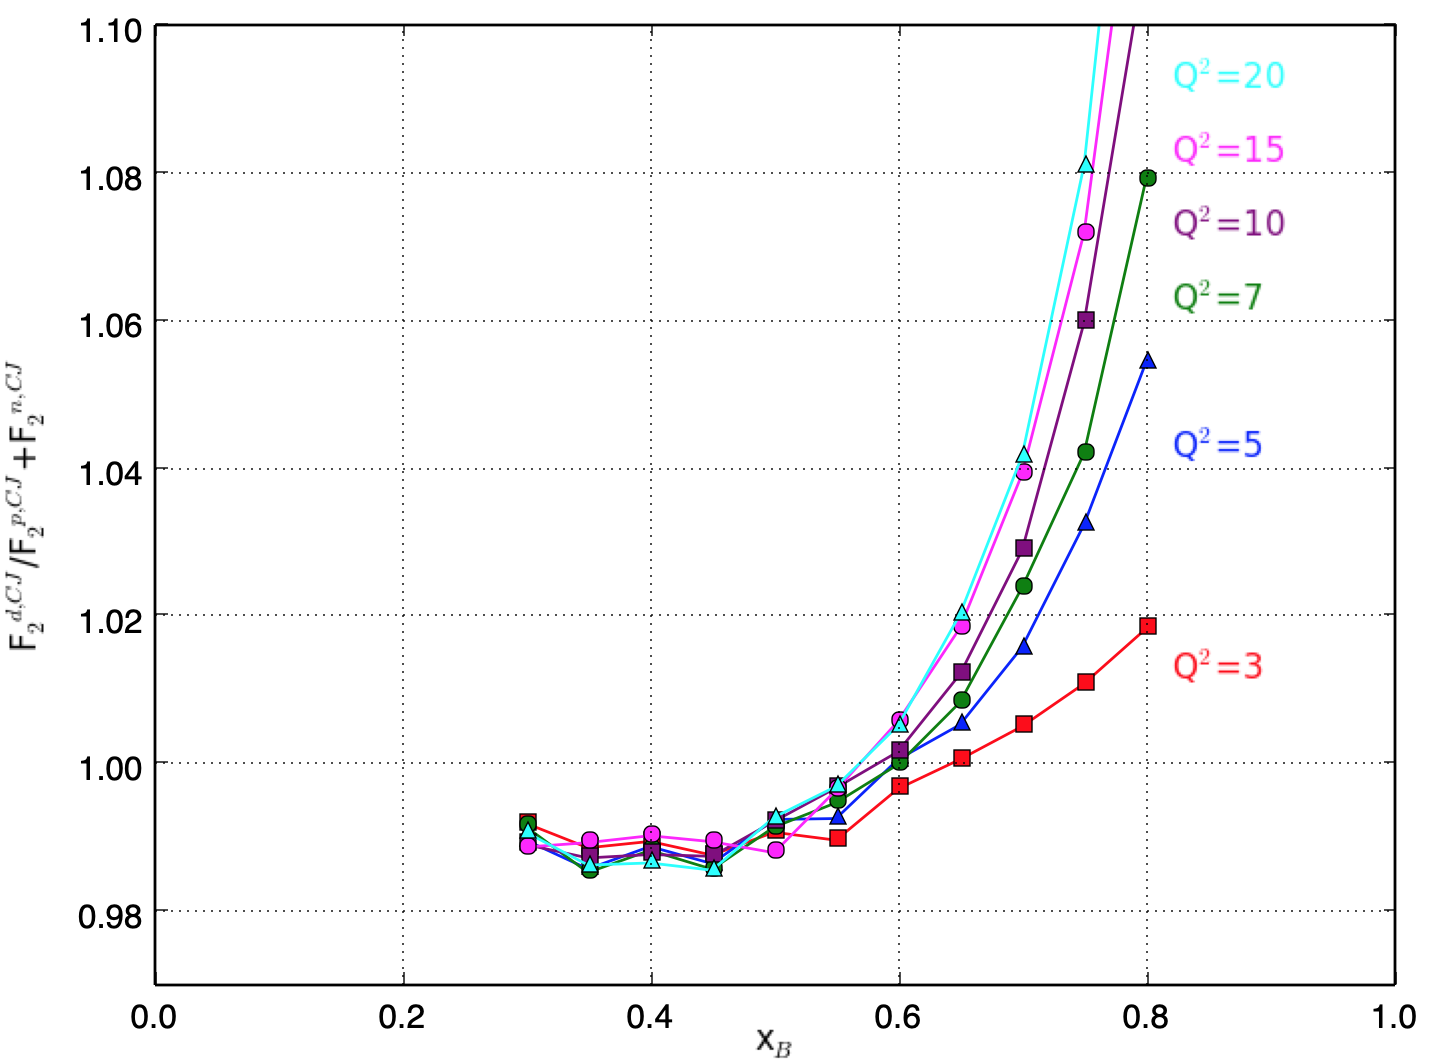
\includegraphics[width=\textwidth]{plots/dpn_allCJ.png}
\end{minipage}\hfill\begin{minipage}{0.5\textwidth}
 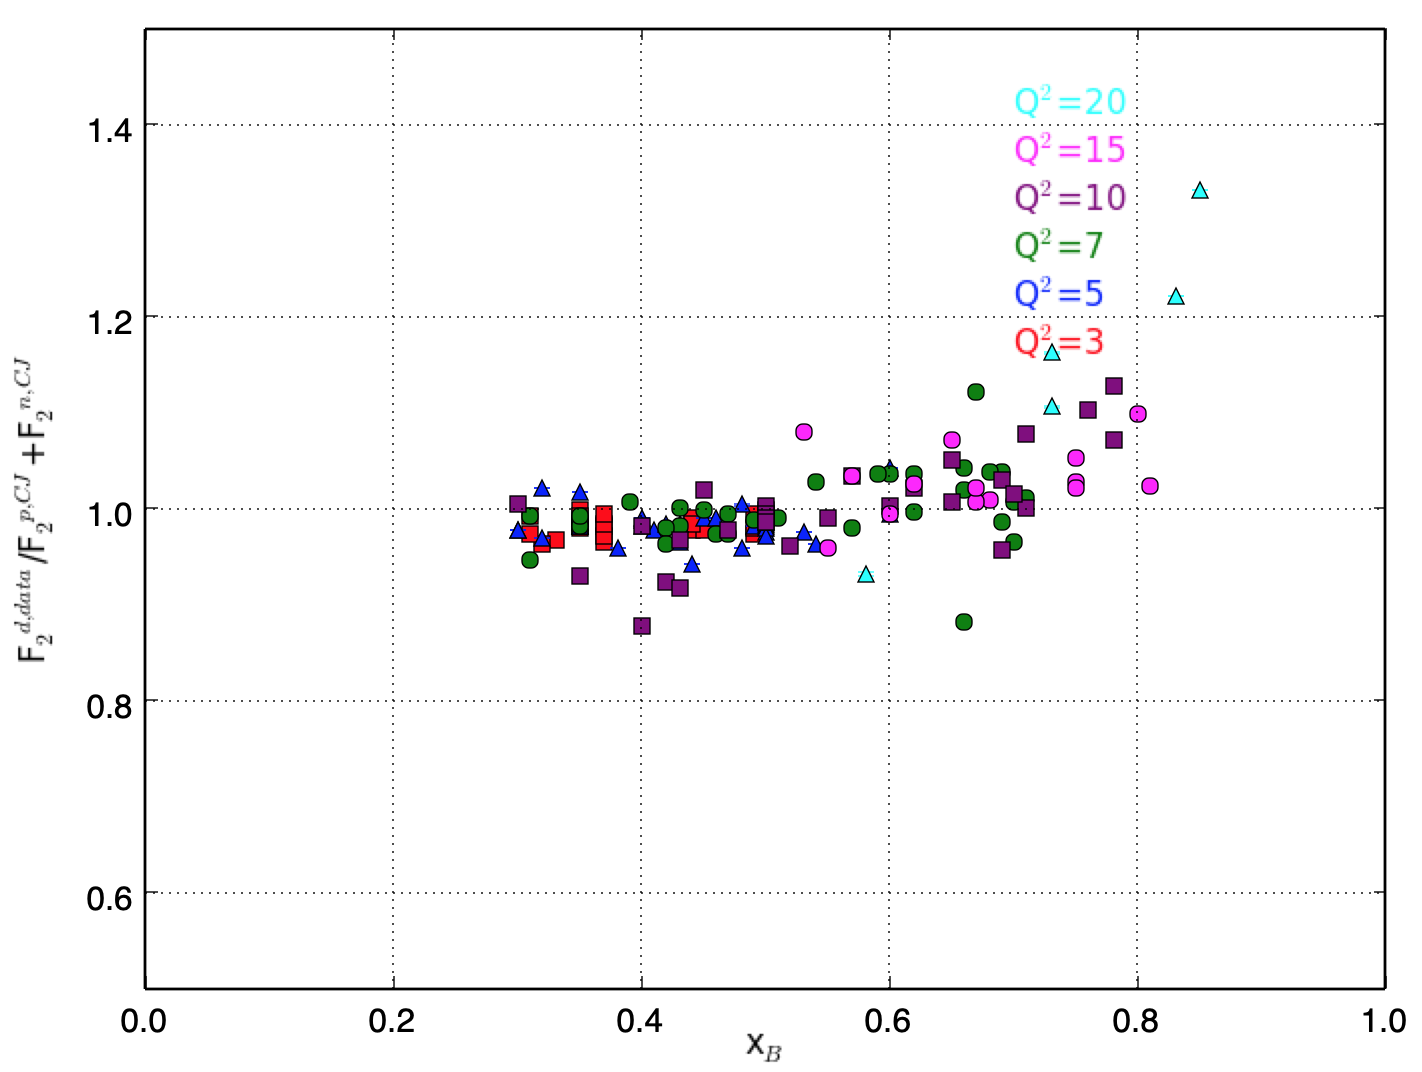
\includegraphics[width=\textwidth]{plots/deuterium_q2.png}
 \end{minipage}
  \caption[]{Left: The deuteron structure function divided by the sum of the free proton and free neutron structure functions from the CJ15 fit is shown for various $Q^2$. This ratio roughly shows the magnitude of the nuclear effects in the deuteron. The $Q^2$ dependence shows significant spread above $x_B=0.6$ where the ratio begins to increase. Right: The global Whitlow deuterium data from SLAC~\cite{XS_d} is shown divided by the sum of the free proton and free neutron structure functions from the CJ15 fit.}
  \label{fig:dpn_cj}
\end{figure}  
 
The same ratio is shown on the right in Fig.~\ref{fig:dpn_cj} using the global Whitlow deuterium data. The same general trend is observed as that shown in the CJ15 where the $Q^2$ has a more significant effect on the ratio at large values of $x_B$. The $F_2^d/F_2^p$ and $F_2^d/F_2^n$ ratios from the CJ15 fit are shown in Fig.~\ref{fig:dratio_cj}. 
 
  \begin{figure}
\begin{minipage}{0.5\textwidth}
 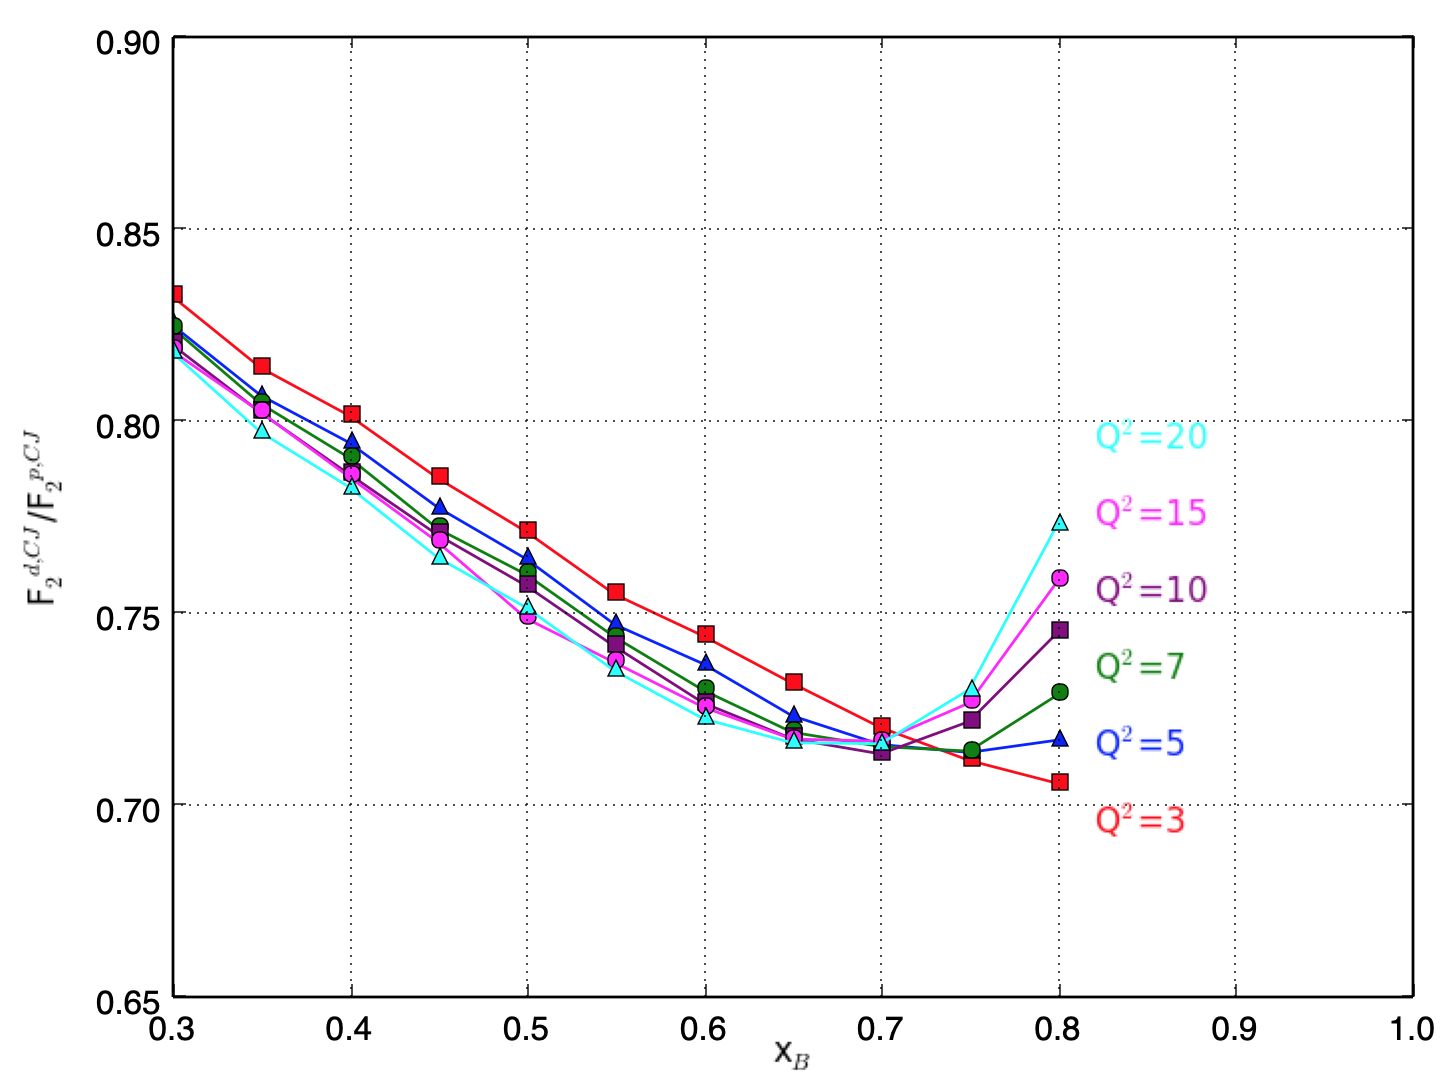
\includegraphics[width=\textwidth]{plots/dpratio_CJ.png}
\end{minipage}\hfill\begin{minipage}{0.5\textwidth}
 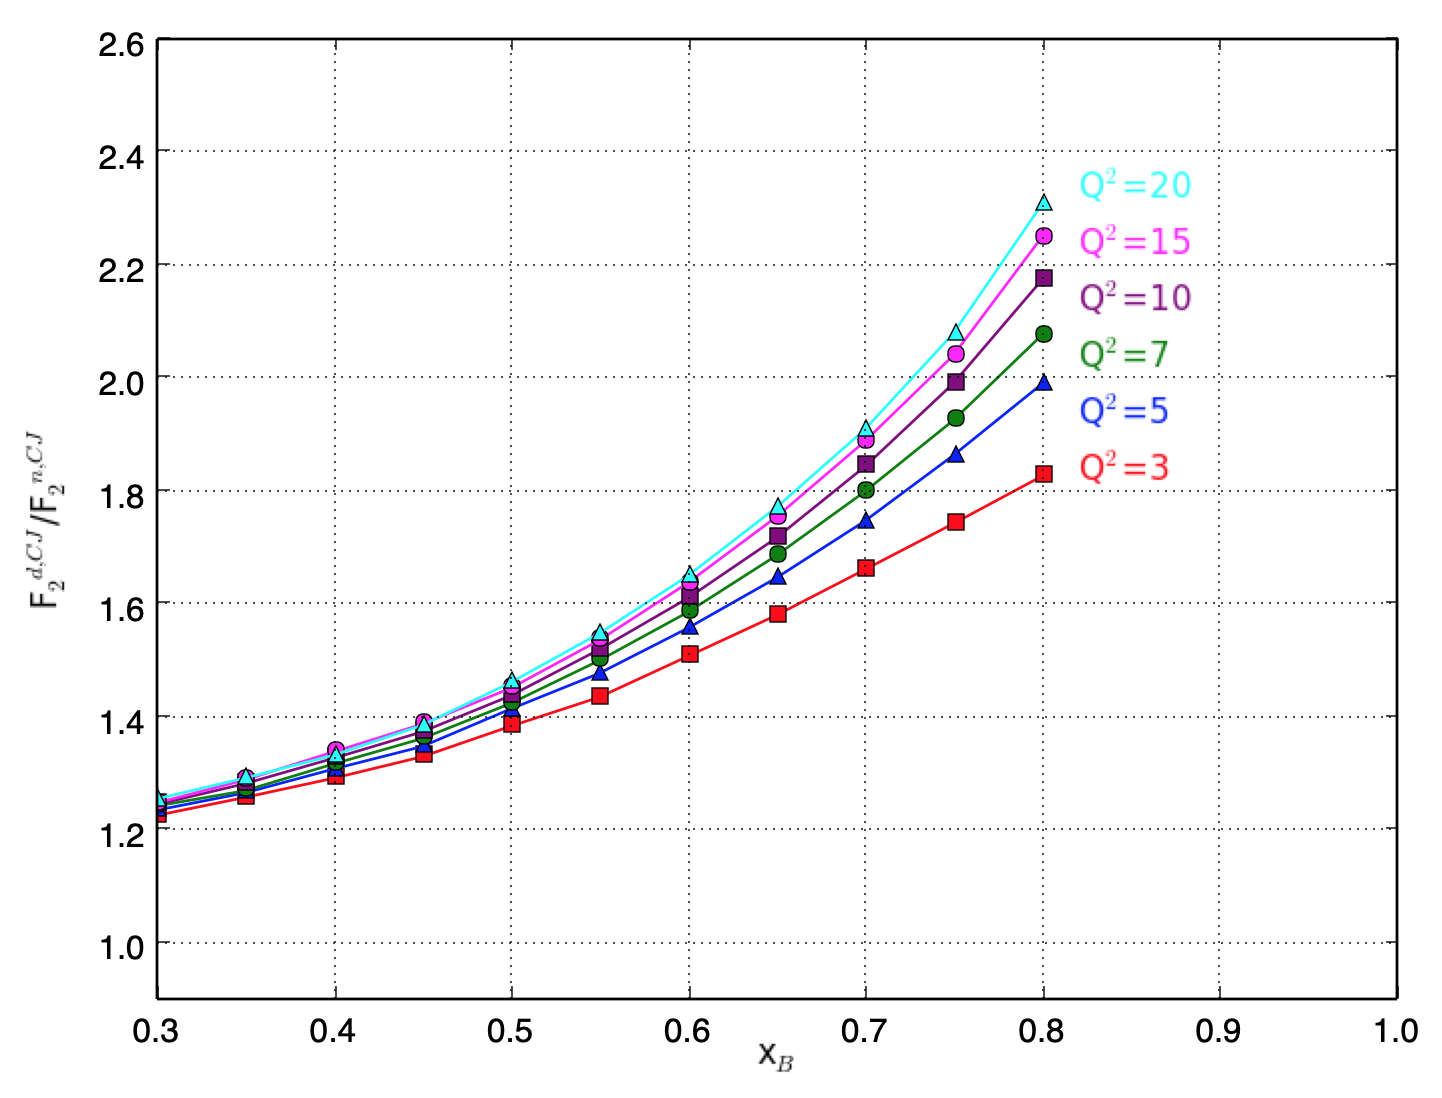
\includegraphics[width=\textwidth]{plots/dnratio_CJ.png}
 \end{minipage}
  \caption[Deuteron ratios from CJ15]{Left: The deuterium structure function from the CJ15 fit is shown as a ratio to the proton structure function from CJ15 for various $Q^2$. Right: The deuterium structure function from the CJ15 fit is shown as a ratio to the neutron structure function from CJ15 for various $Q^2$.}
  \label{fig:dratio_cj}
\end{figure} 

The significance of the spread in ratios at large $x_B$ values is that many experiments, SLAC E139 included, did not observe a large $Q^2$ dependence in the data and so the points were averaged in $Q^2$ for each point in $x_B$. Additionally, the EMC Effect is characterized by a linear fit in the range of $x_B$ from 0.3--0.7 where deuterium clearly exhibits non-linear nuclear modification effects. These two observations affect the interpretation and extraction of the EMC Effect. 

\section{Structure function extraction from the E139 cross sections}

Most experiments only publish the extracted $F_2$ ratios. For this analysis, the experimental cross sections were desirable for the flexibility to construct and study the $F_2$ ratios for the nucleus of interest relative to free nucleon quantities. The SLAC E139 experiment published the experimental cross sections for the following nuclei: deuterium, helium, beryllium, carbon, aluminum, calcium, iron, silver and gold. The cross sections include published statistical and systematic errors. The $F_2$ structure function for each nucleus is extracted from the cross section using the relationship shown in Equation~\eqref{eq:f2eqn}.

\begin{equation}
F_2 = \dfrac{d^2\sigma}{d\Omega dE'}\dfrac{1+R}{1+\epsilon R}\dfrac{K\nu}{4\pi^2\alpha\Gamma (1+\nu^2/Q^2)}
\label{eq:f2eqn}
\end{equation}

From Equation~\eqref{eq:f2eqn}, $\epsilon$, $K$, and $\Gamma$ are defined by the usual quantities of the electron scattering kinematics in Equation~\eqref{eq:f2eqndetails}. These quantities include the measured scattering angle $\theta$, the momentum transfer $Q^2$, the energy transfer $\nu$, the scattered electron energy $E'$, the mass of the proton $M$, and the squared invariant mass $W^2$. $R$ is determined from the R1990 fit to world data.

\begin{align}
\epsilon=&(1+2\dfrac{\nu^2+Q^2}{Q^2}tan^2\dfrac{\theta}{2})^{-1}\\
K=&\dfrac{W^2-M^2}{2M}\\
\Gamma=&\dfrac{\alpha KE'}{2\pi^2Q^2E(1-\epsilon)}
\label{eq:f2eqndetails}
\end{align}

For most published cross section ratios, corrections are applied to account for the excess of neutrons in asymmetric nuclei. This correction is referred to as the ``isoscalar correction" and is defined in Equation~\eqref{eq:isocorr}. While this correction is not applied in this paper for the $F_2$ ratios per free proton and free neutron, it is relevant for accurately reconstructing the published $F_2^A$/$F_2^d$ cross sections as in most analyses. 

\begin{equation}
f_{iso}^A = \dfrac{\dfrac{1}{2}(1+F_2^n/F_2^p)}{\dfrac{1}{A}(Z+(A-Z)F_2^n/F_2^p)}
\label{eq:isocorr}
\end{equation}

From the analysis described in this section, the carbon and gold $F_2^A/F_2^d$ ratios are reconstructed (with the iso-scalar correction applied to gold) and compared to the published ratios in the EMC and NMC experiments as shown in Fig.~\ref{fig:emc_ratios}.

\begin{figure}[H]
  \centering
      	  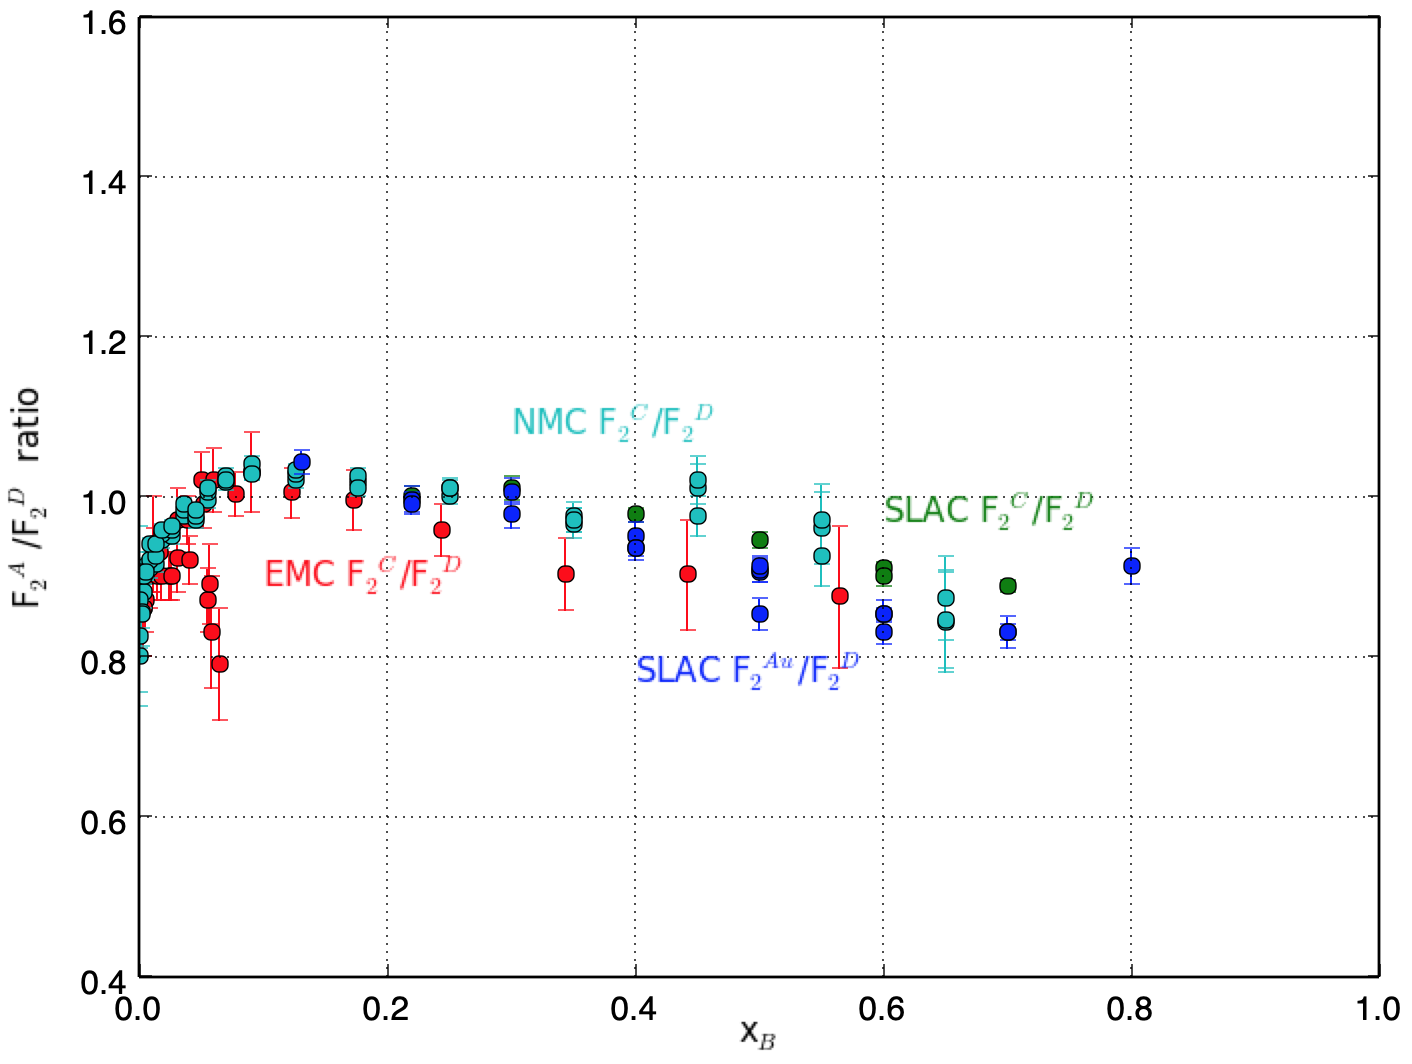
\includegraphics[width=0.5\textwidth]{plots/emc_ratios_data.png}
 	 \caption[EMC ratios for various data]{The published structure function ratios per nucleon for carbon and gold are shown from SLAC, NMC, and the EMC experiments.}
  \label{fig:emc_ratios}
 \end{figure}
 
 The carbon ratio from the SLAC E139 experiment is consistent with the ratio found in the EMC and NMC experiments, and the carbon exhibits a shallower slope with respect to $x_B$ as compared to the heavier, iso-scalar corrected gold ratio. 

\section{General observations}

The standard EMC structure function ratio is compared with ratios of the structure function of the nucleus to that of the free proton and free neutron, separately. The $F_2^A/F_2^d$ ratios for the carbon and gold nuclei are shown in Fig.~\ref{fig:data_np_ratio} using the collective world data as published in Ref.~\ref{Malace:2014uea}. The gold nucleus (heavier than carbon) exhibits a steeper slope as a standard observation of the EMC Effect. The $F_2^A/AF_2^p$ ratio is the per nucleon ratio to the proton structure function and is also shown in Fig.~\ref{fig:data_np_ratio}. These ratios are consistent with theory predictions and exhibit a similar trend to the ratio of the structure function to deuterium in that the slope steepens for heavier nuclei. The vertical spread in the ratios of the various nuclei lessens when an iso-scalar correction is applied. The $F_2^p$ structure function is obtained from the CJ15 fit.      
 
  \begin{figure}
\begin{minipage}{0.5\textwidth}
 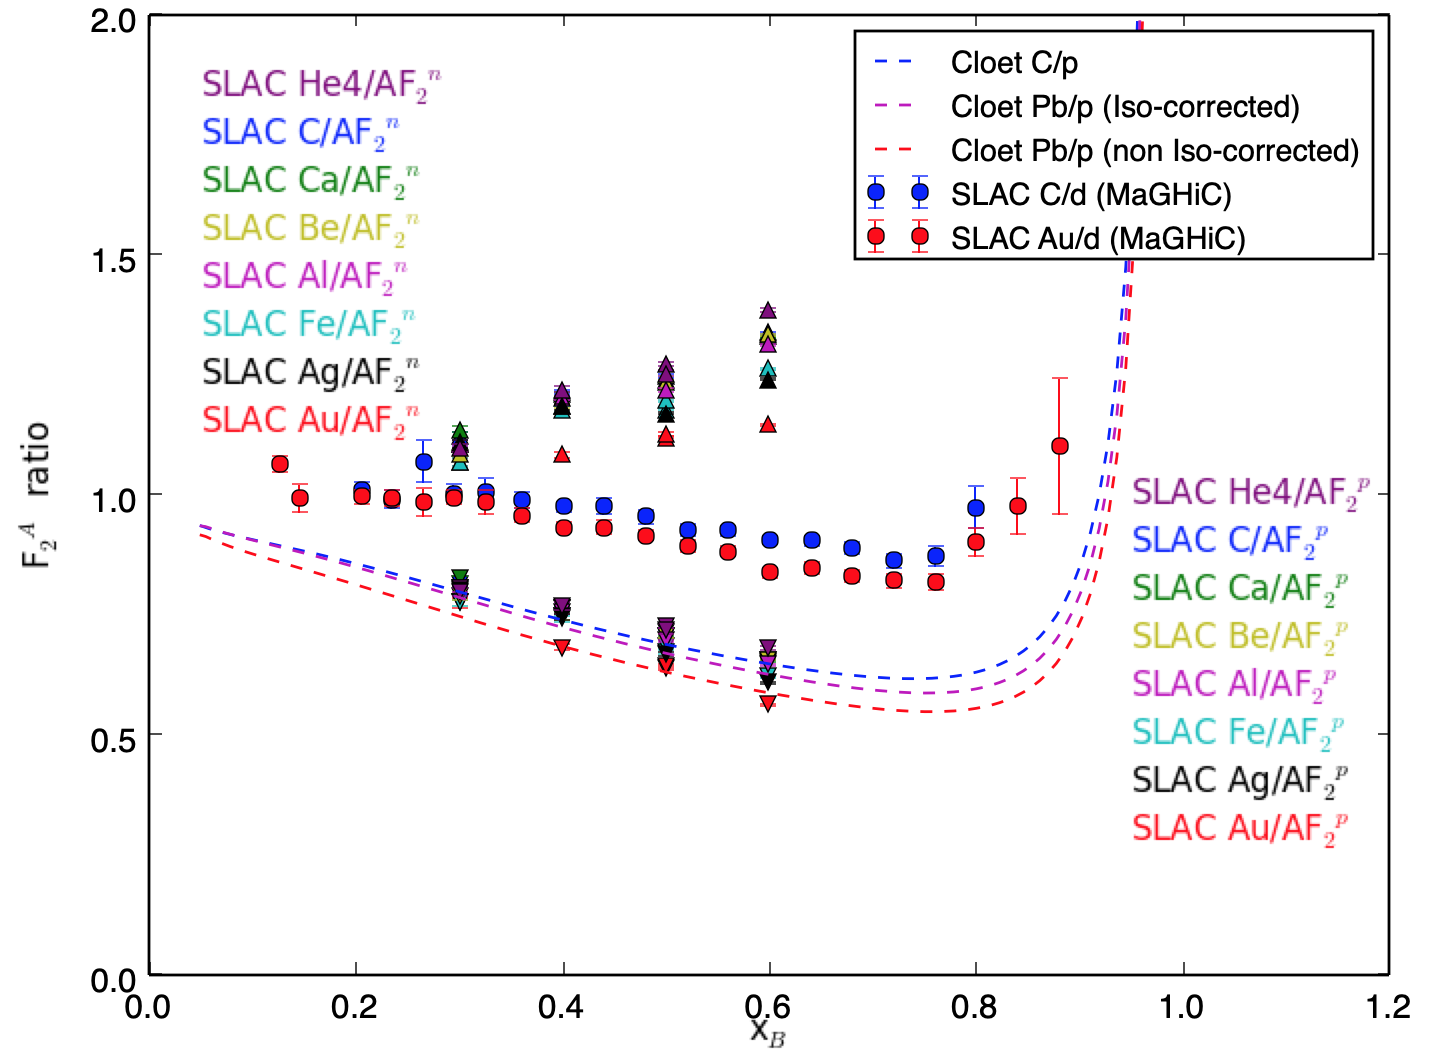
\includegraphics[width=\textwidth]{plots/Anp_data_ratio.png}
\end{minipage}\hfill\begin{minipage}{0.5\textwidth}
 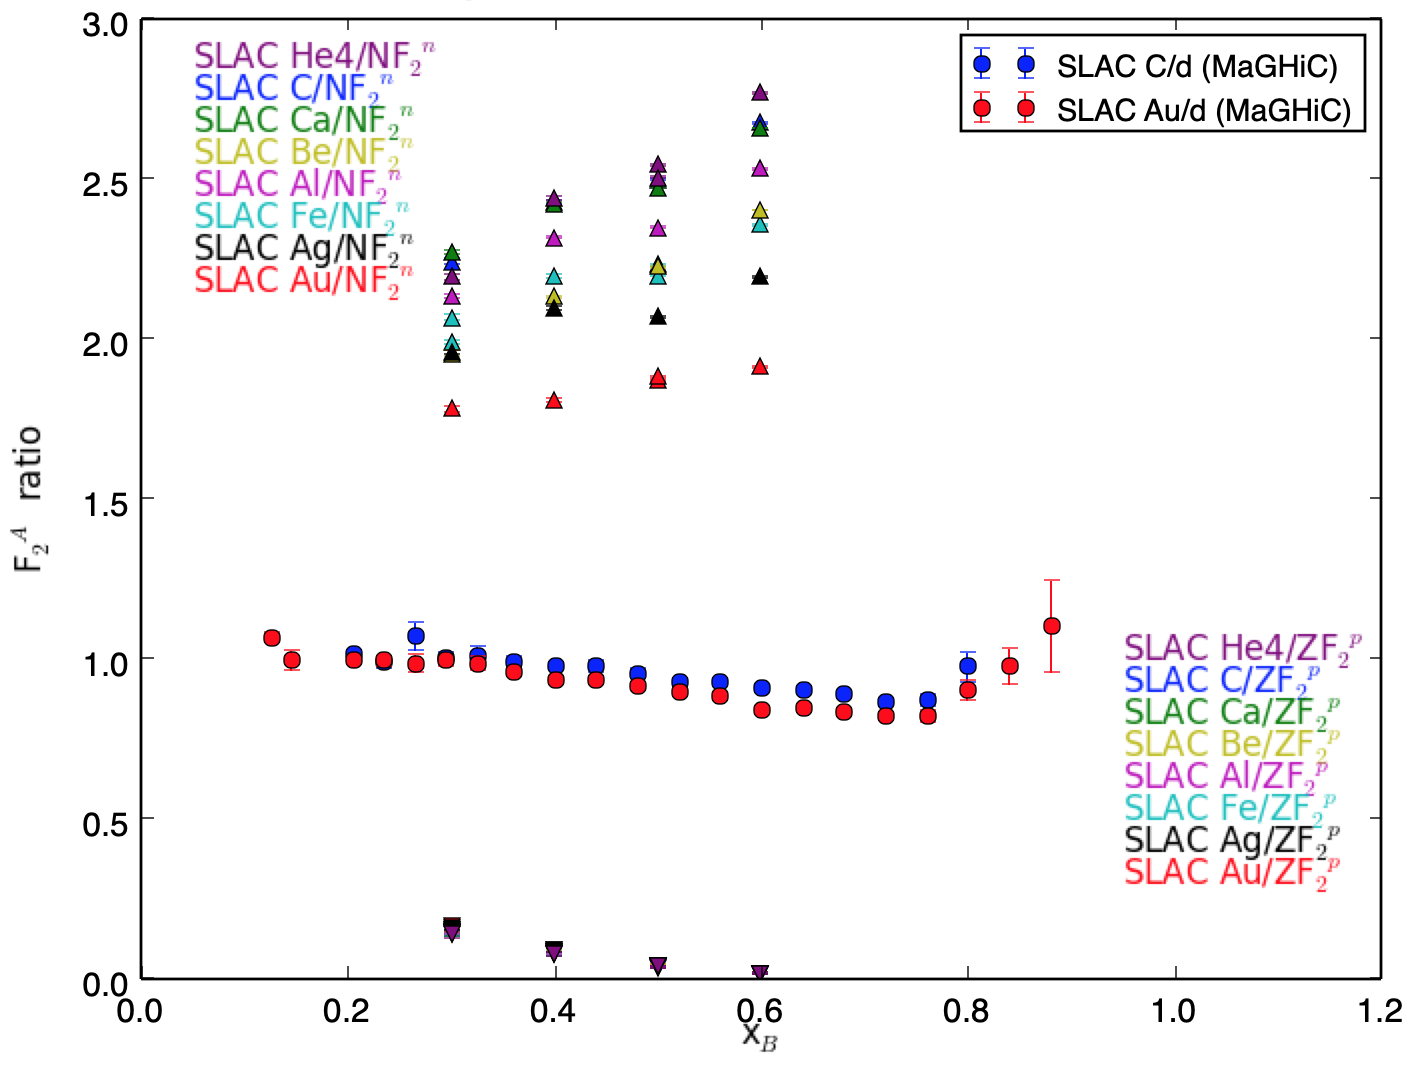
\includegraphics[width=\textwidth]{plots/AZNnp_data_ratio.png}
 \end{minipage}
  \caption[$F_2^A$ ratio to $F_2^n$ and $F_2^p$]{Left: $F_2^A$ calculated from the published SLAC E139 cross sections is taken as a ratio per nucleon to $F_2^n$ and $F_2^p$, separately. The published EMC ratios for carbon and gold~\cite{Malace:2014uea} are shown for reference as $F_2^A/F_2^d$ per nucleon. Theory predictions for the $F_2^A$ structure function per nucleon as a ratio to $F_2^p$ are shown. Right: $F_2^A$ calculated from the published SLAC E139 cross sections is taken as a ratio per neutron or proton and $F_2^n$ and $F_2^p$, separately. The published EMC ratios for carbon and gold~\cite{Malace:2014uea} are shown for reference.}
  \label{fig:data_np_ratio}
\end{figure}  
 
The $F_2^A/AF_2^n$ ratio is the per nucleon to the free neutron. The free neutron $F_2^n$ is from the CJ15 fit to the world data. As shown in Fig.~\ref{fig:data_np_ratio}, the $F_2^A/AF_2^n$ ratios for the SLAC E139 nuclei exhibit a significantly larger vertical spread when compared to the vertical spread of the $F_2^A/AF_2^p$ ratios for various nuclei. The  $F_2^A/AF_2^n$ ratios also exhibit a positive slope in contrast to the ratios constructed using the free proton. These observations are further magnified on the right in Fig.~\ref{fig:data_np_ratio} where the ratios for each nuclei are shown as per proton ($F_2^A/ZF_2^p$) and per neutron ($F_2^A/NF_2^n$). 
 
\section{Deuterium nuclear effects and heavier nuclei}
\subsection{Deuterium}
%plots: include d/n or n/d of Whitlow+BONUS to show Q2 dependency
The nuclear effects in deuterium are non-negligible for values of $x_B$ from 0.3--0.7 in the region of interest to the EMC Effect. The nuclear effects in deuterium can be quantified somewhat as the difference between the sum of the free proton and free neutron to that of the measured deuterium structure function. In Fig.~\ref{fig:fits_D}, the $F_2^A$ ratio is defined in two ways: the standard $F_2^A/F_2^d$ (shown in blue) and $F_2^A/ZF_2^p+(A-Z)F_2^n$ (shown in red). The SLAC E139 data was taken for $Q^2$ of 5, 10, and 15 GeV$^2$.

 \begin{figure}
\begin{minipage}{0.5\textwidth}
 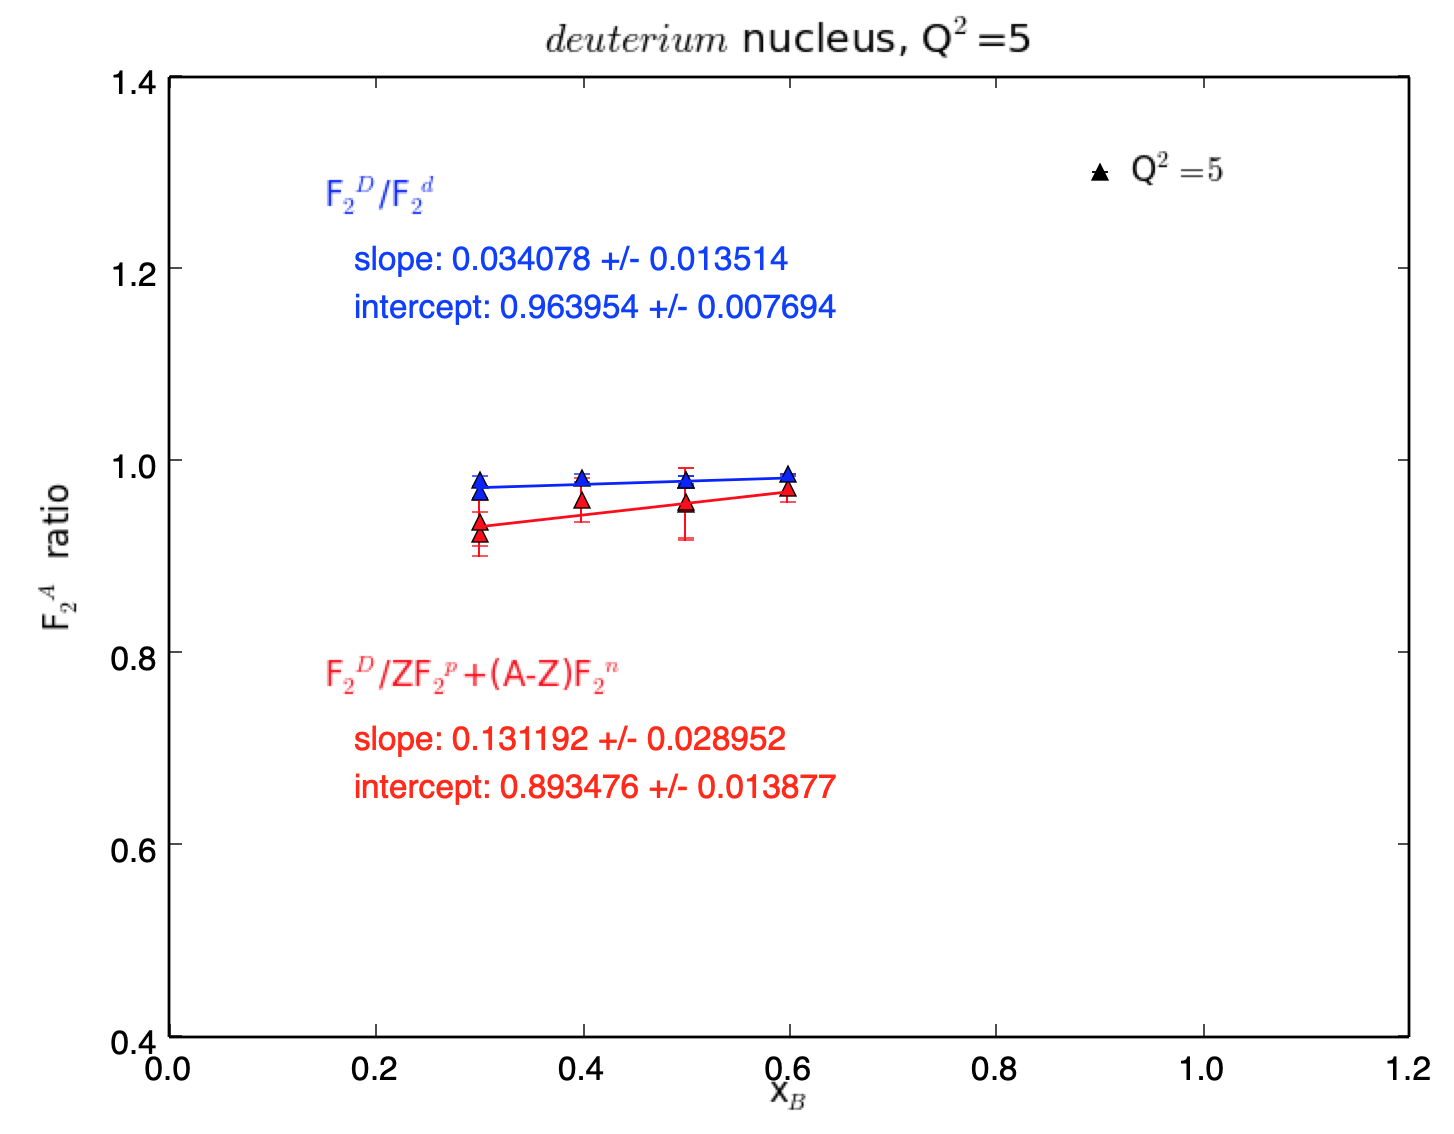
\includegraphics[width=\textwidth]{plots/q2_5/q2_5_D.png}
\end{minipage}\hfill\begin{minipage}{0.5\textwidth}
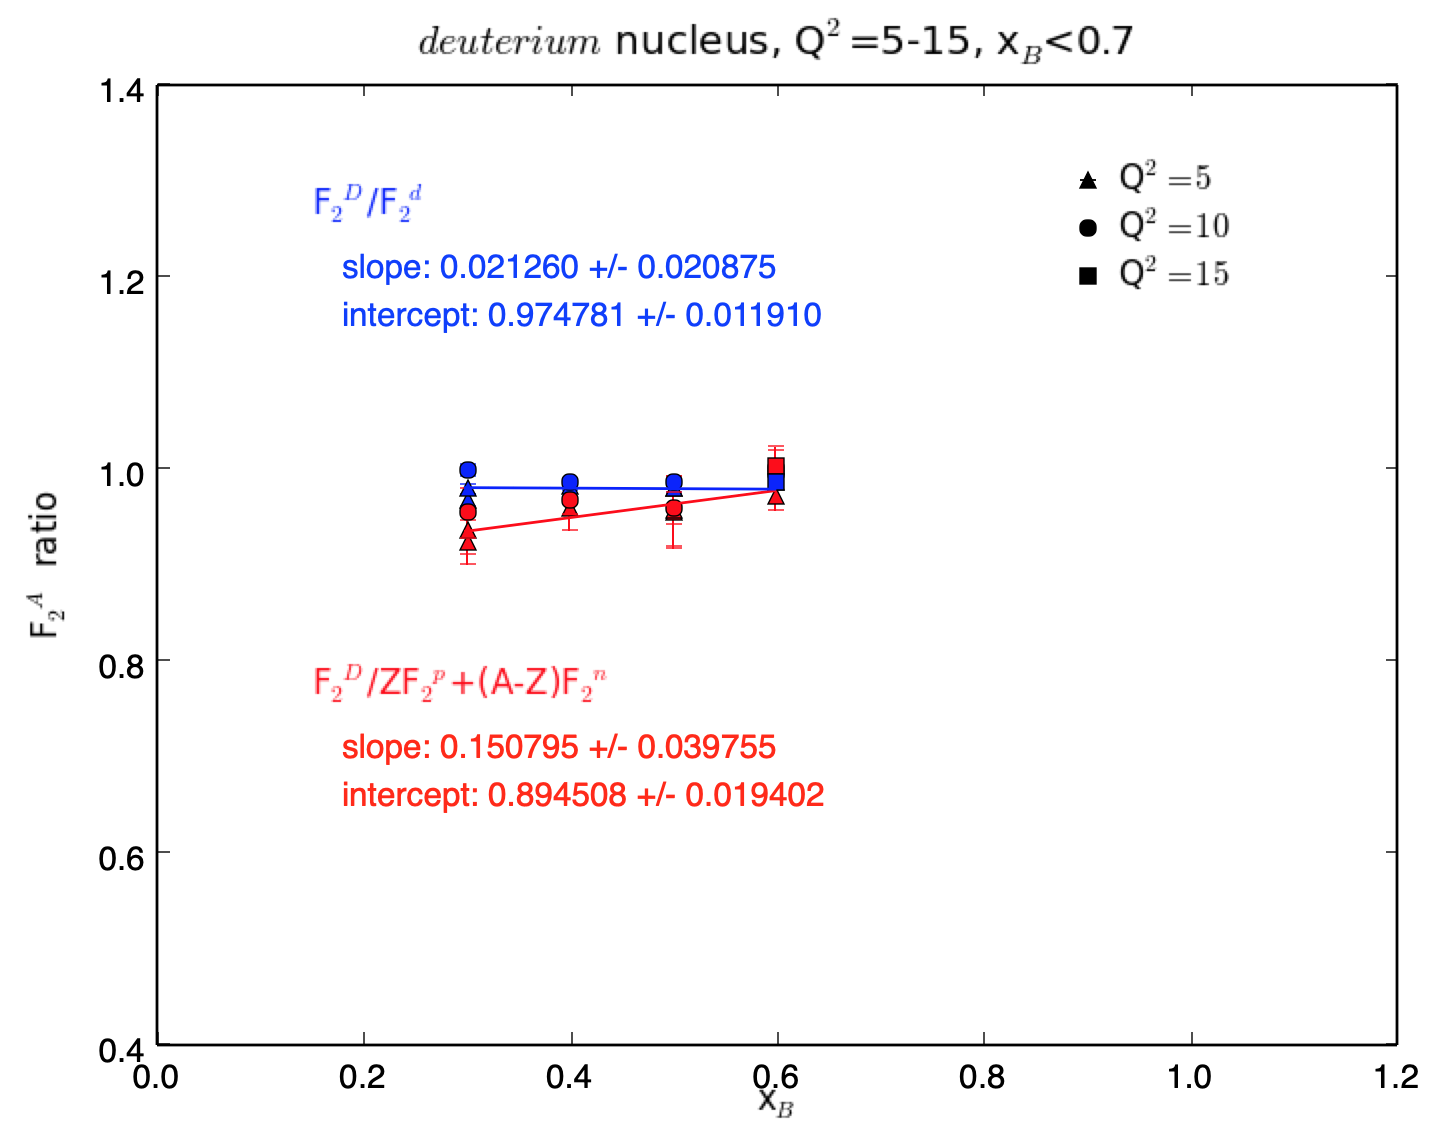
\includegraphics[width=\textwidth]{plots/q2_all_x_l7/q2_all_x_l7_D.png}
\end{minipage}\hfill\begin{minipage}{0.5\textwidth}
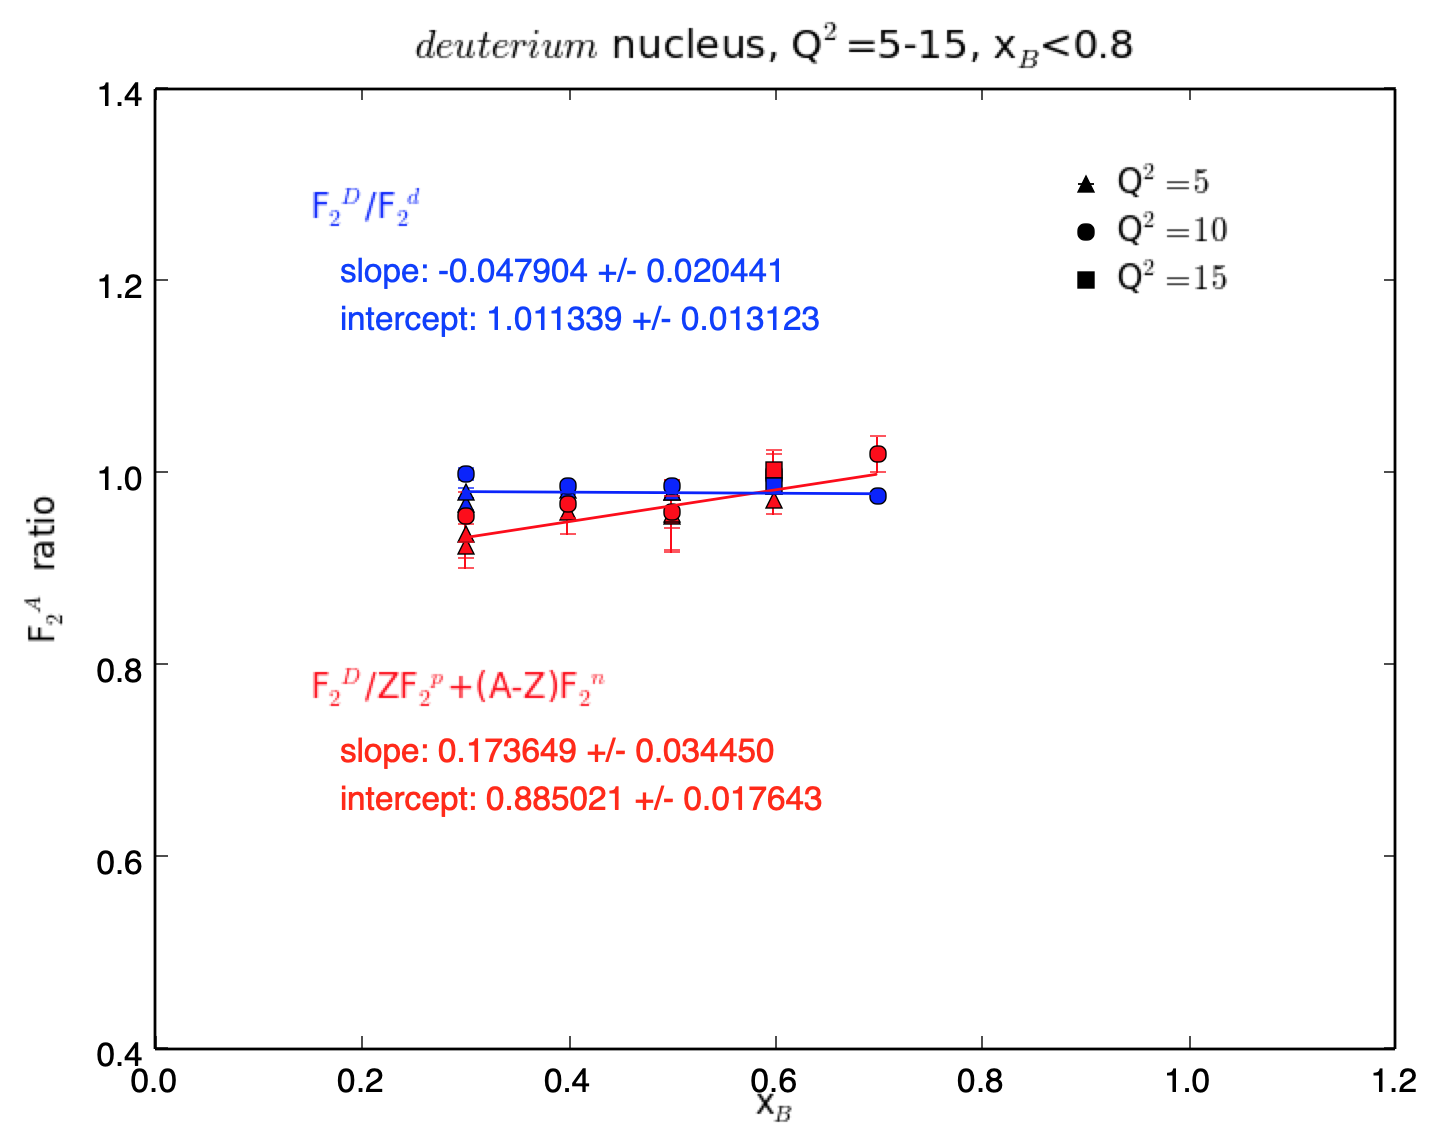
\includegraphics[width=\textwidth]{plots/q2_all_x_all/all_D.png}
\end{minipage}
  \caption[]{Linear fits to the deuterium target data with cuts on $Q^2$ and $x_B$. The blue data shows the ratio of the E139 nucleus relative to the CJ15 deuterium while the red data shows the ratio of the E139 nucleus relative to the sum of the free proton and free neutron (excluding nuclear effects of deuterium). Top left: linear fit to the data taken for $Q^2=5$ GeV$^2$. Top Right: linear fit to the data taken for all $Q^2$ but excluding the data at $x_B=0.7$. Bottom: linear fit to all data taken through $x_B=0.7$.}
  \label{fig:fits_D}
\end{figure}  

In Fig.~\ref{fig:fits_D}, the deuterium ratios from the SLAC E139 data are shown using the CJ15 structure function constructs in the denominators. The different $Q^2$ data are shown using different shapes in each plot, and fits to the ratios are taken separately including and excluding the highest $x_B$ point at 0.7. There is a systematic offset from unity for deuterium taken as a ratio to itself, but the ratio is relatively flat across $x_B$. There exists a clear difference between the ratio taken relative to the deuteron structure function (blue) and the ratio taken relative to sum of the free neutron and free proton structure functions (red). The difference also exhibits a small spread in $Q^2$.  

\subsection{Heavier nuclei}

The ratios for all the target nuclei in the SLAC E139 experiment are compared where the denominator is deuterium and the denominator is the sum of the free proton and neutron contributions. Carbon is a symmetric nucleus, and the results are shown in Fig.~\ref{fig:fits_C}. 

 \begin{figure}
\begin{minipage}{0.5\textwidth}
 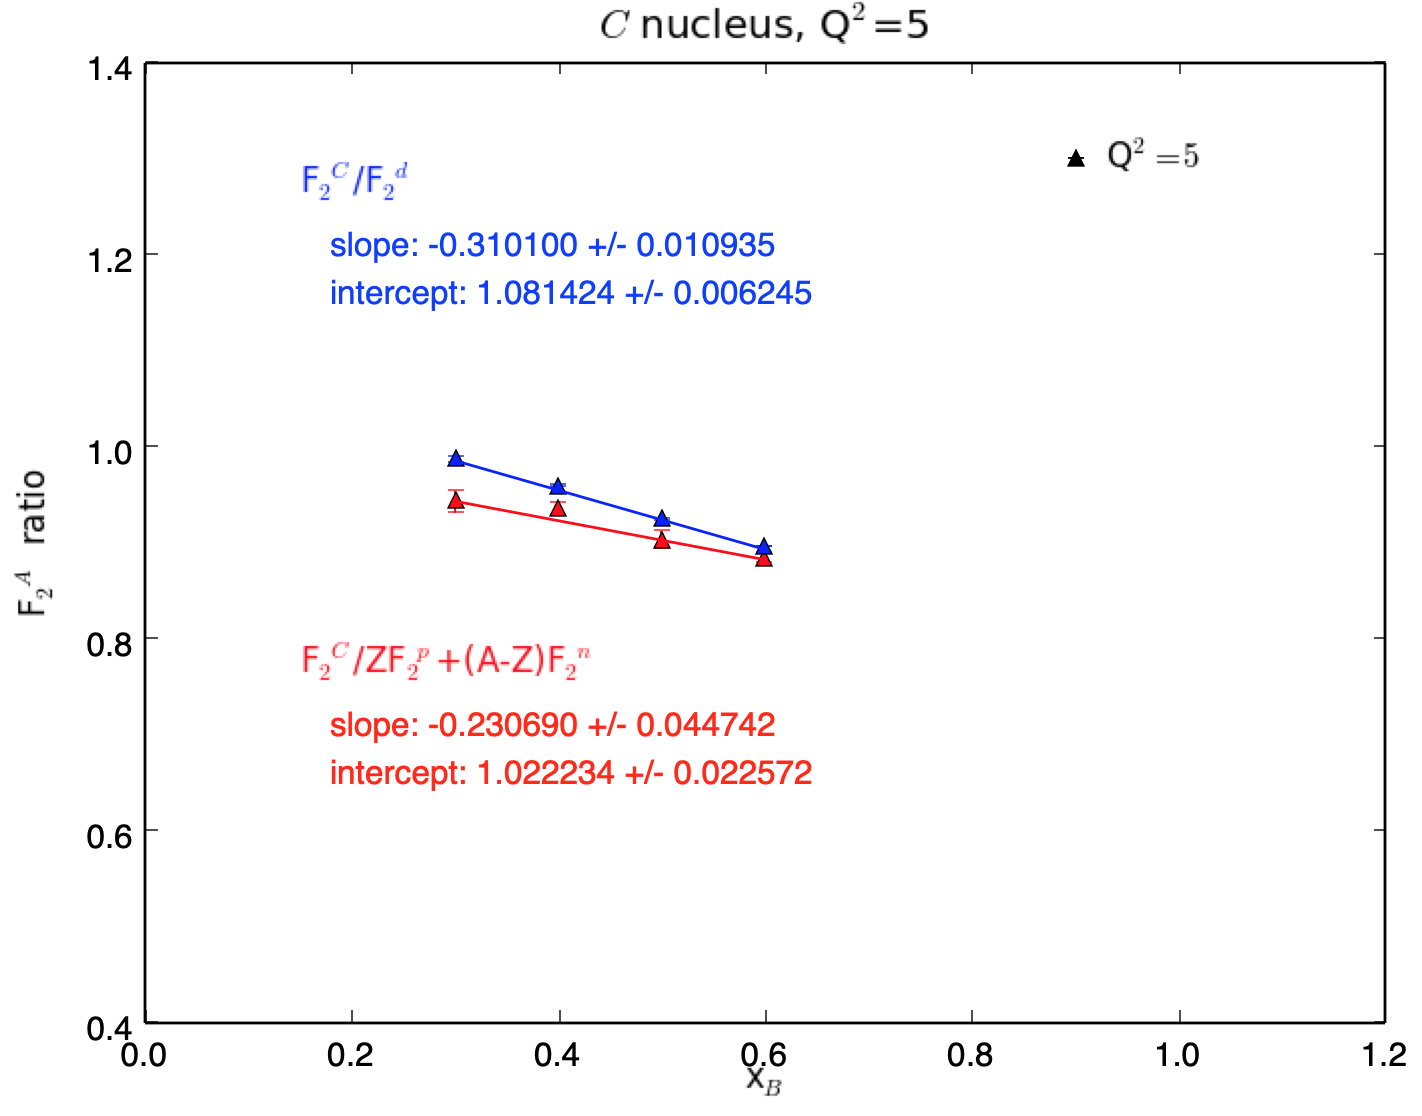
\includegraphics[width=\textwidth]{plots/q2_5/q2_5_C.png}
\end{minipage}\hfill\begin{minipage}{0.5\textwidth}
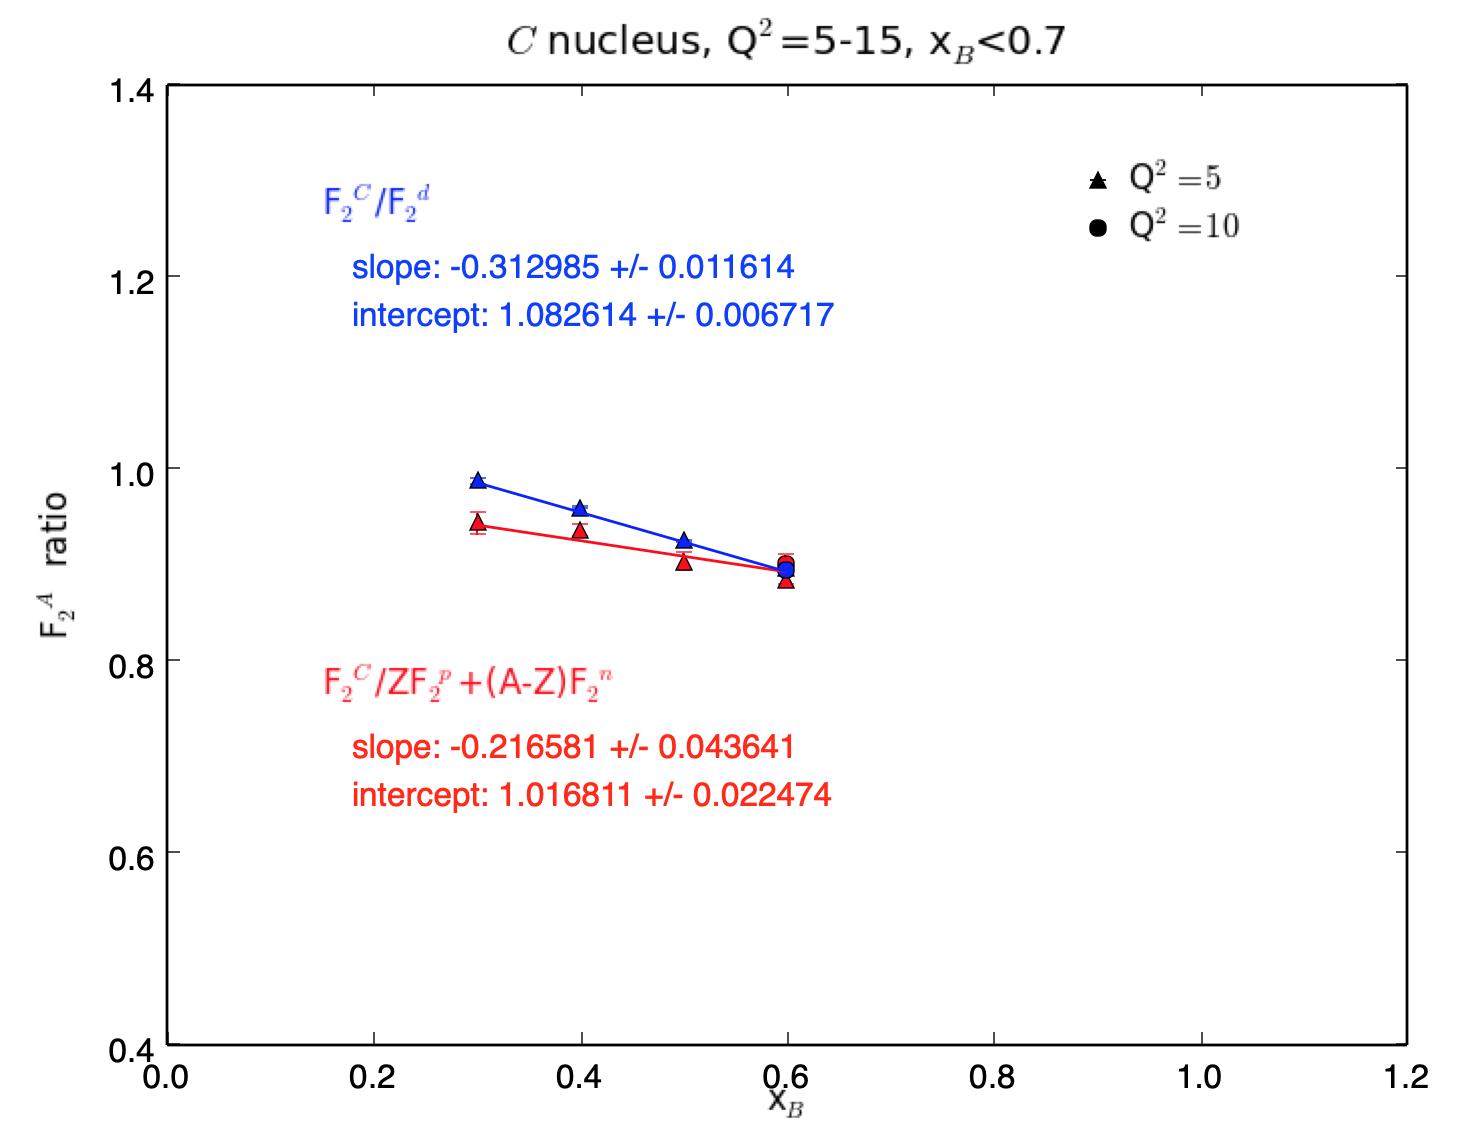
\includegraphics[width=\textwidth]{plots/q2_all_x_l7/q2_all_x_l7_C.png}
%\end{minipage}\hfill\begin{minipage}{0.5\textwidth}
%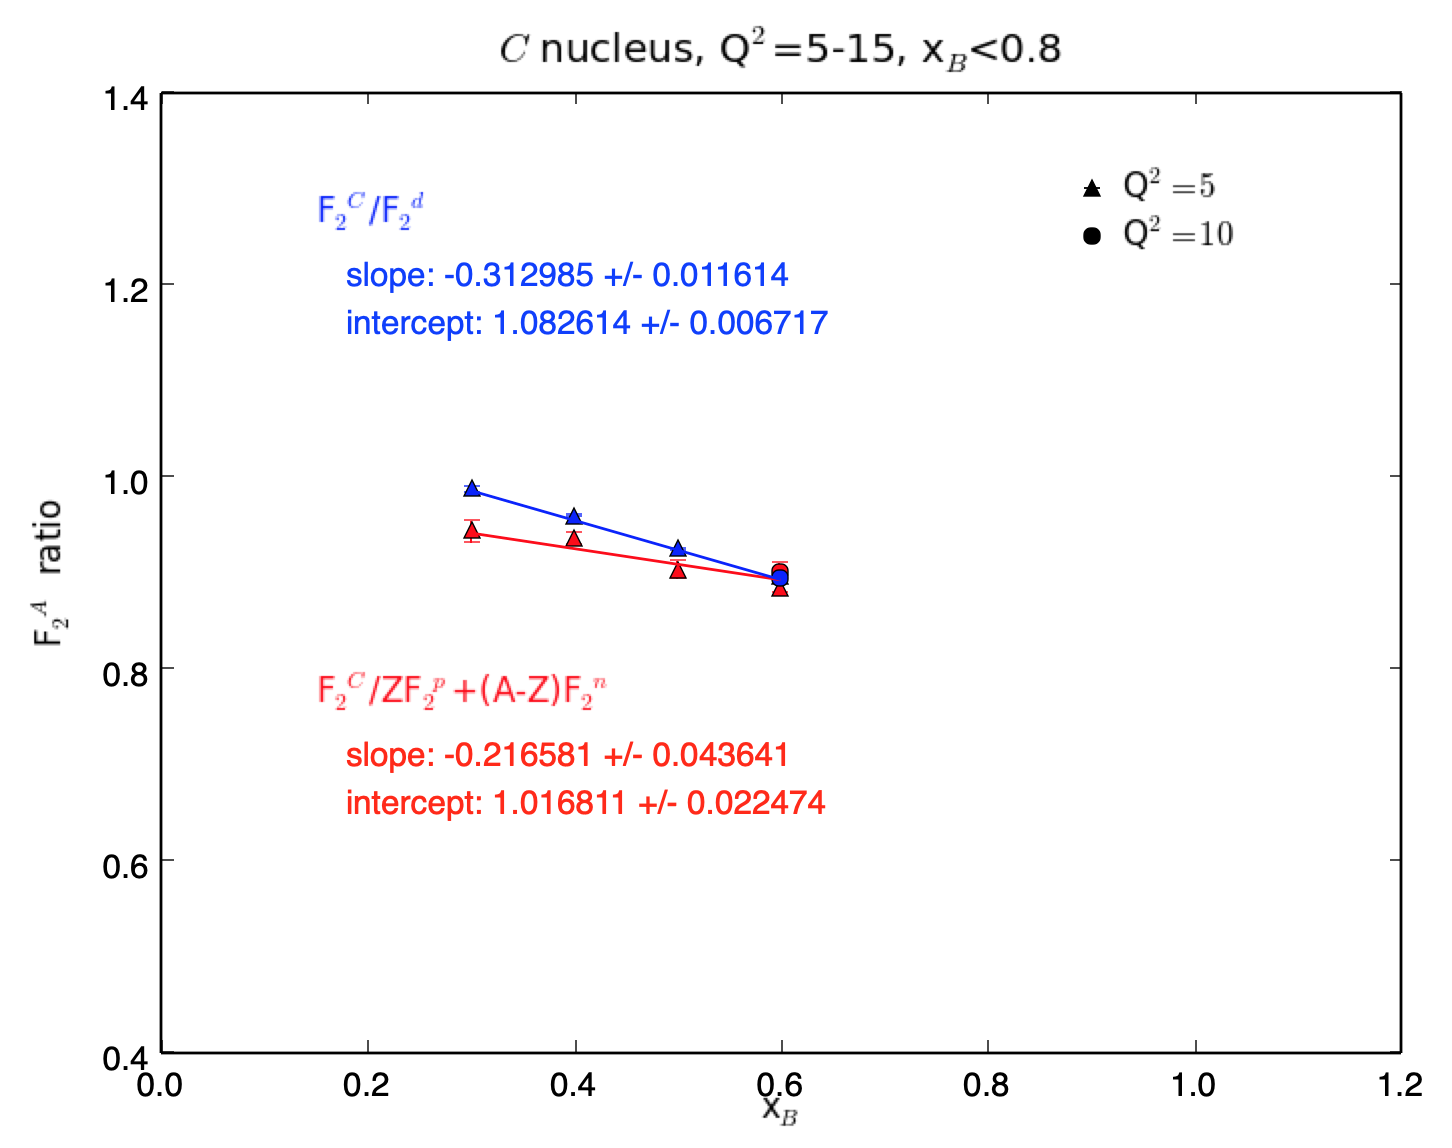
\includegraphics[width=\textwidth]{plots/q2_all_x_all/all_C.png}
\end{minipage}
  \caption[]{Linear fits to the $C$ target data with cuts on $Q^2$ and $x_B$. The blue data shows the ratio of the nucleus relative to deuterium while the red data shows the ratio of the nucleus relative to the sum of the free proton and free neutron (excluding nuclear effects of deuterium). Left: linear fit to the data taken for $Q^2=5$ GeV$^2$. Right: linear fit to the data taken for all $Q^2$ but excluding the data at $x_B=0.7$. No data was taken in the E139 experiment for carbon at $x_B=0.7$.}
  \label{fig:fits_C}
\end{figure}   

No data was taken in the E139 experiment for carbon at $x_B>0.6$. The slope is steeper for the ratio taken with respect to the sum of the free neutron and free proton components. A more extreme case is seen in the gold nucleus in Fig.~\ref{fig:fits_Au}. 

 \begin{figure}
\begin{minipage}{0.5\textwidth}
 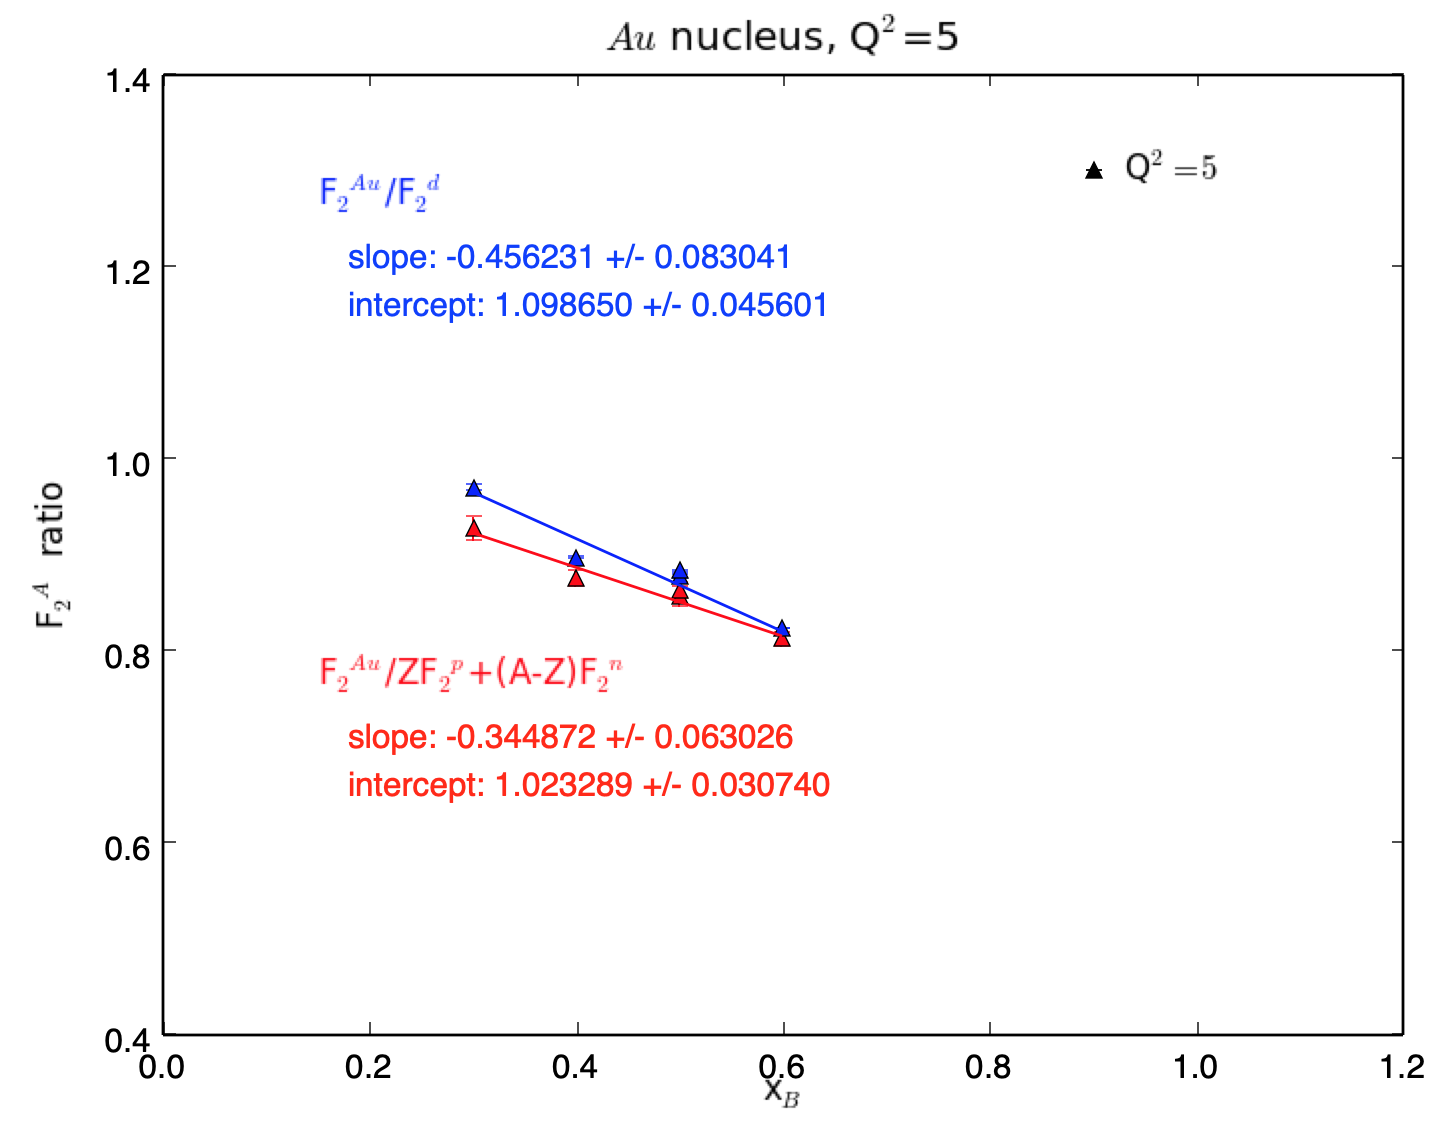
\includegraphics[width=\textwidth]{plots/q2_5/q2_5_Au.png}
\end{minipage}\hfill\begin{minipage}{0.5\textwidth}
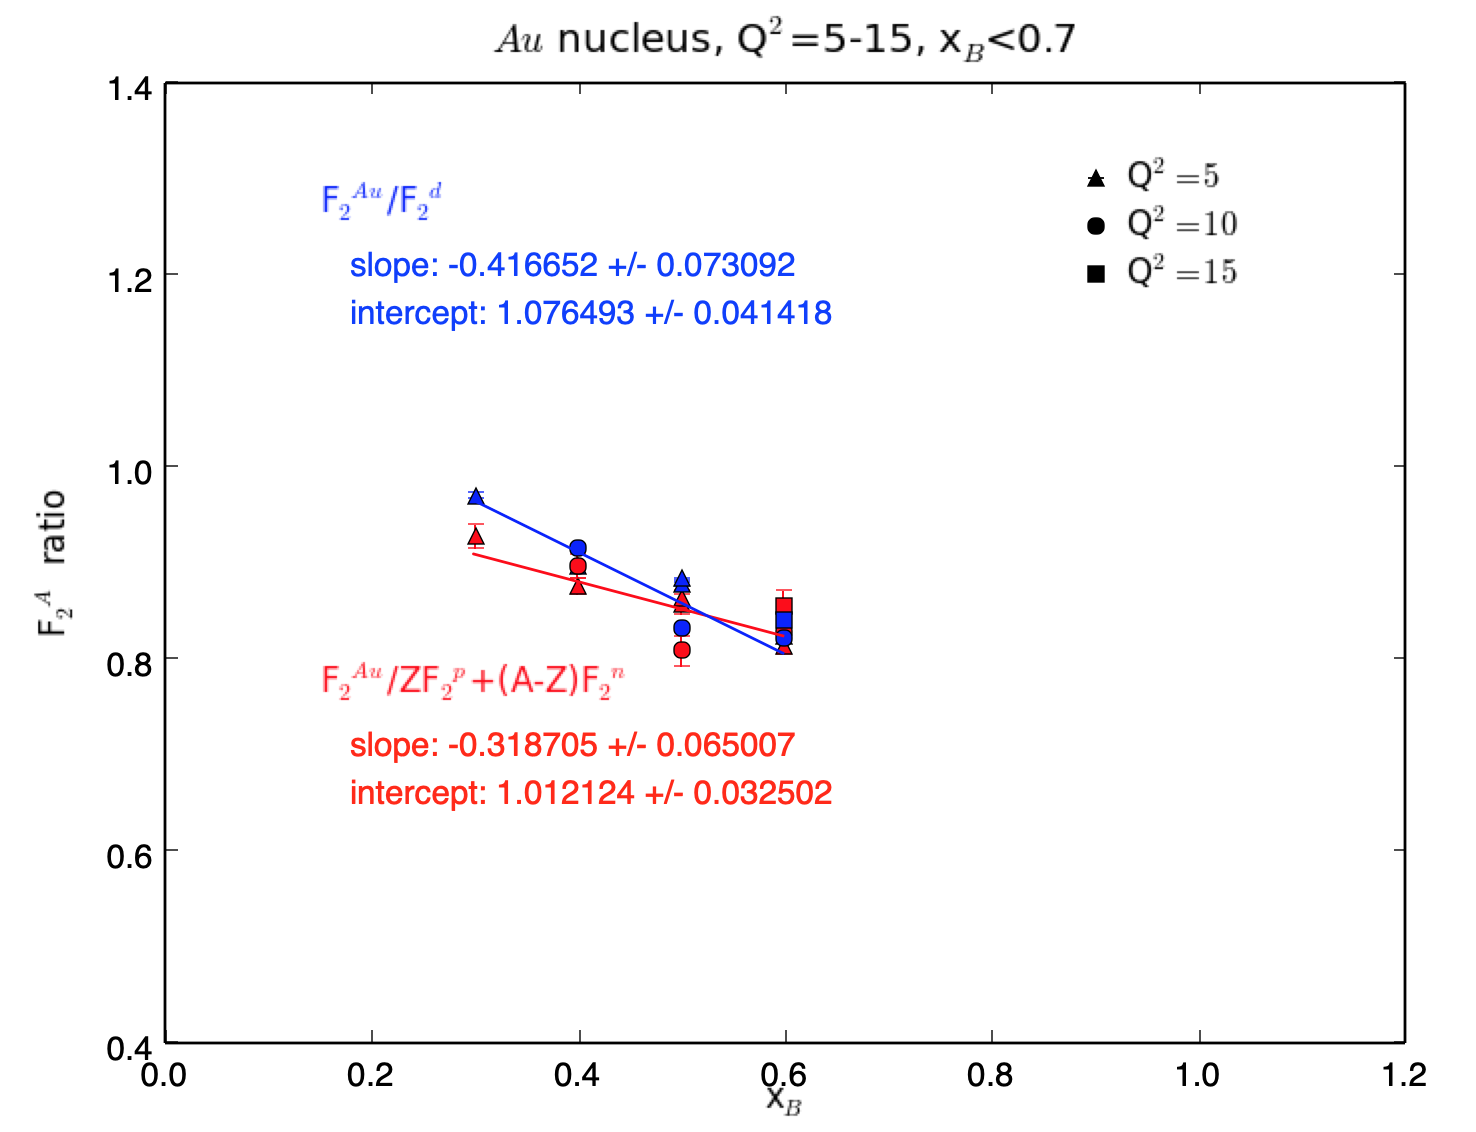
\includegraphics[width=\textwidth]{plots/q2_all_x_l7/q2_all_x_l7_Au.png}
\end{minipage}\hfill\begin{minipage}{0.5\textwidth}
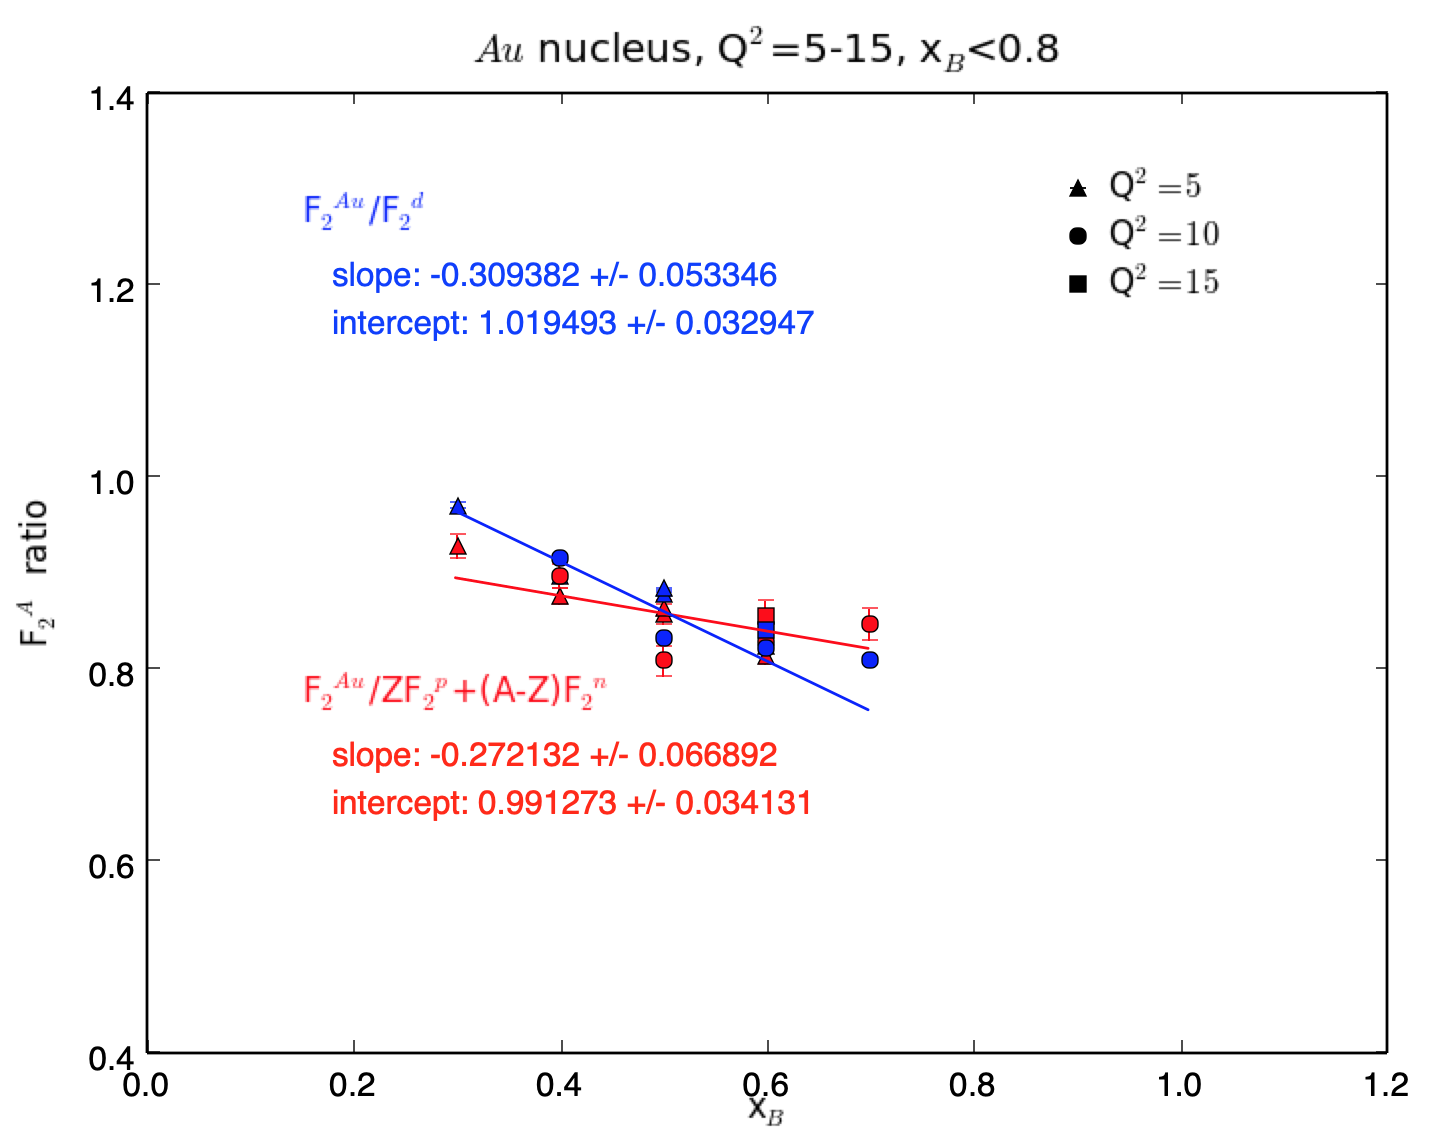
\includegraphics[width=\textwidth]{plots/q2_all_x_all/all_Au.png}
\end{minipage}
  \caption[]{Linear fits to the $Au$ target data with cuts on $Q^2$ and $x_B$. The blue data shows the ratio of the nucleus relative to deuterium while the red data shows the ratio of the nucleus relative to the sum of the free proton and free neutron (excluding nuclear effects of deuterium). Top left: linear fit to the data taken for $Q^2=5$ GeV$^2$. Top Right: linear fit to the data taken for all $Q^2$ but excluding the data at $x_B=0.7$. Bottom: linear fit to all data taken through $x_B=0.7$.}
  \label{fig:fits_Au}
\end{figure}   

For the gold nucleus, the slope of the fit the ratio taken with respect to the free neutron and free proton is shallower than the slope taken with respect to deuterium (as consistent with the general trend observed in carbon). When data is fitted for a range of $Q^2$ values, a noticeable striping at each point in $x_B$ is apparent. Furthermore, the higher $x_B$ data (also higher $Q^2$), no longer sit linearly with respect to the lower $x_B$ data. In all nuclei (see Appendix), this discrepancy is most apparent for values of $x_B$ at 0.7. This observation is similar to where one would expect to see the contributions from the deuteron nuclear effects as shown in Fig.~\ref{fig:dn_theory}. Similar fits are made to all the nuclei (shown in the Appendix). The resultant slopes are shown in Tables~\ref{SlopeFits}, \ref{SlopeFits1}, and \ref{SlopeFits2}. The slopes are shown as a function of $A$ for the nuclei in  Fig.~\ref{fig:Aslope_summary}.

  \begin{figure}[H]
\begin{minipage}{0.5\textwidth}
 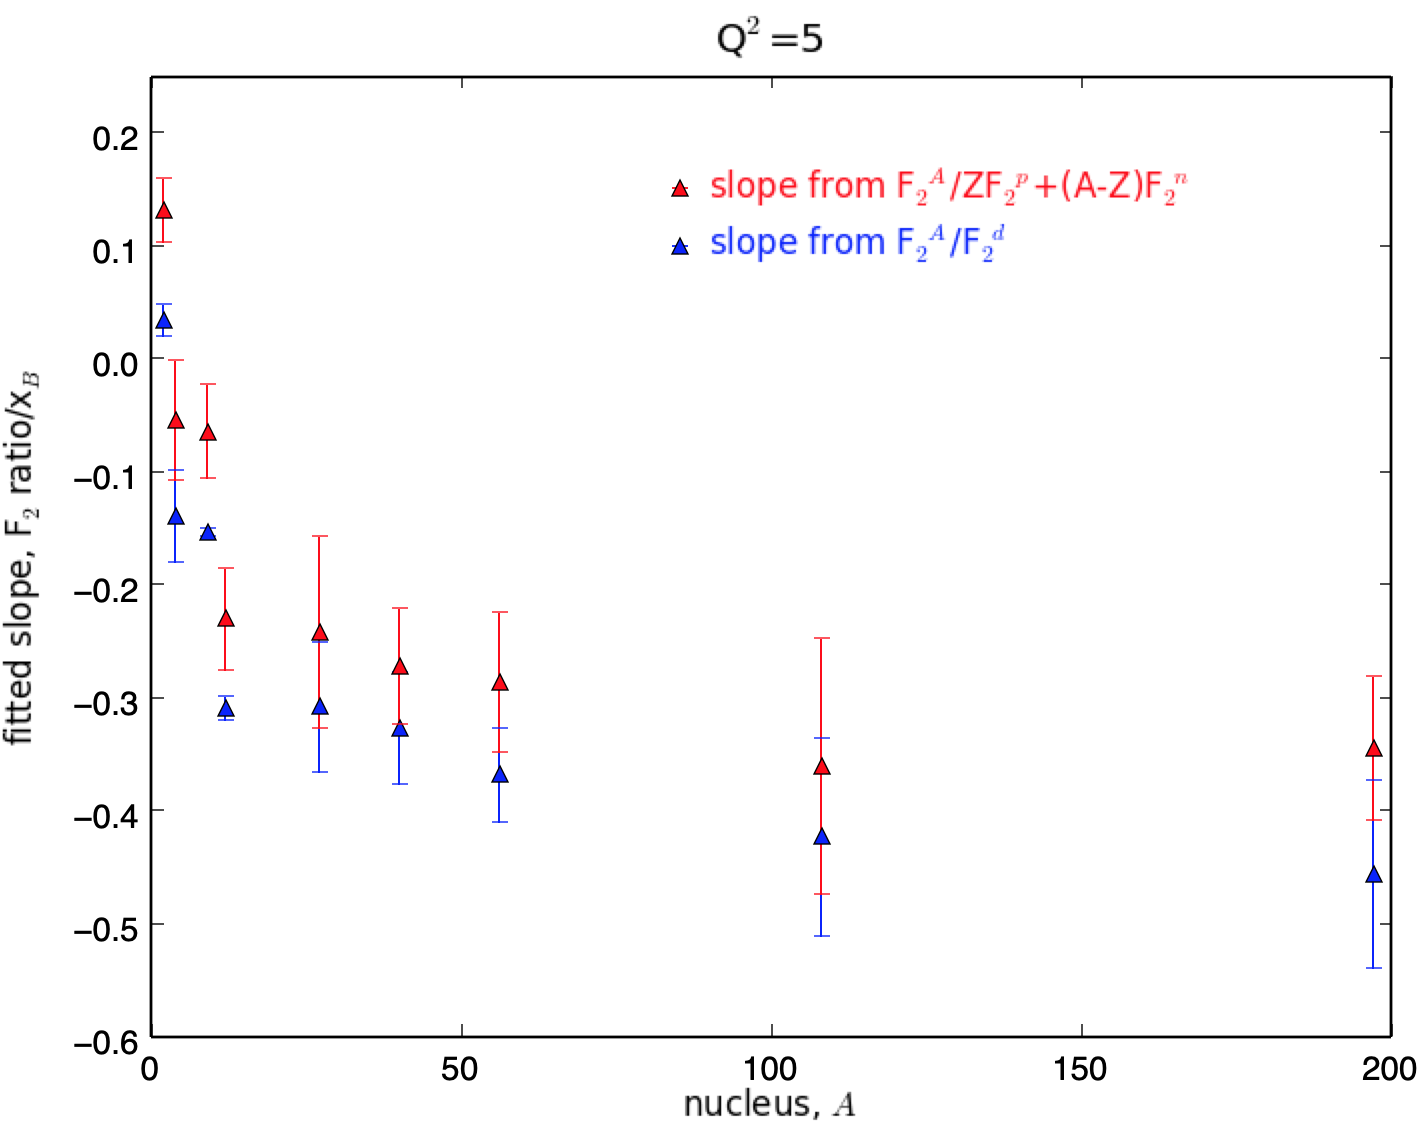
\includegraphics[width=\textwidth]{plots/plotsvA/Aslope_q5.png}
\end{minipage}\hfill\begin{minipage}{0.5\textwidth}
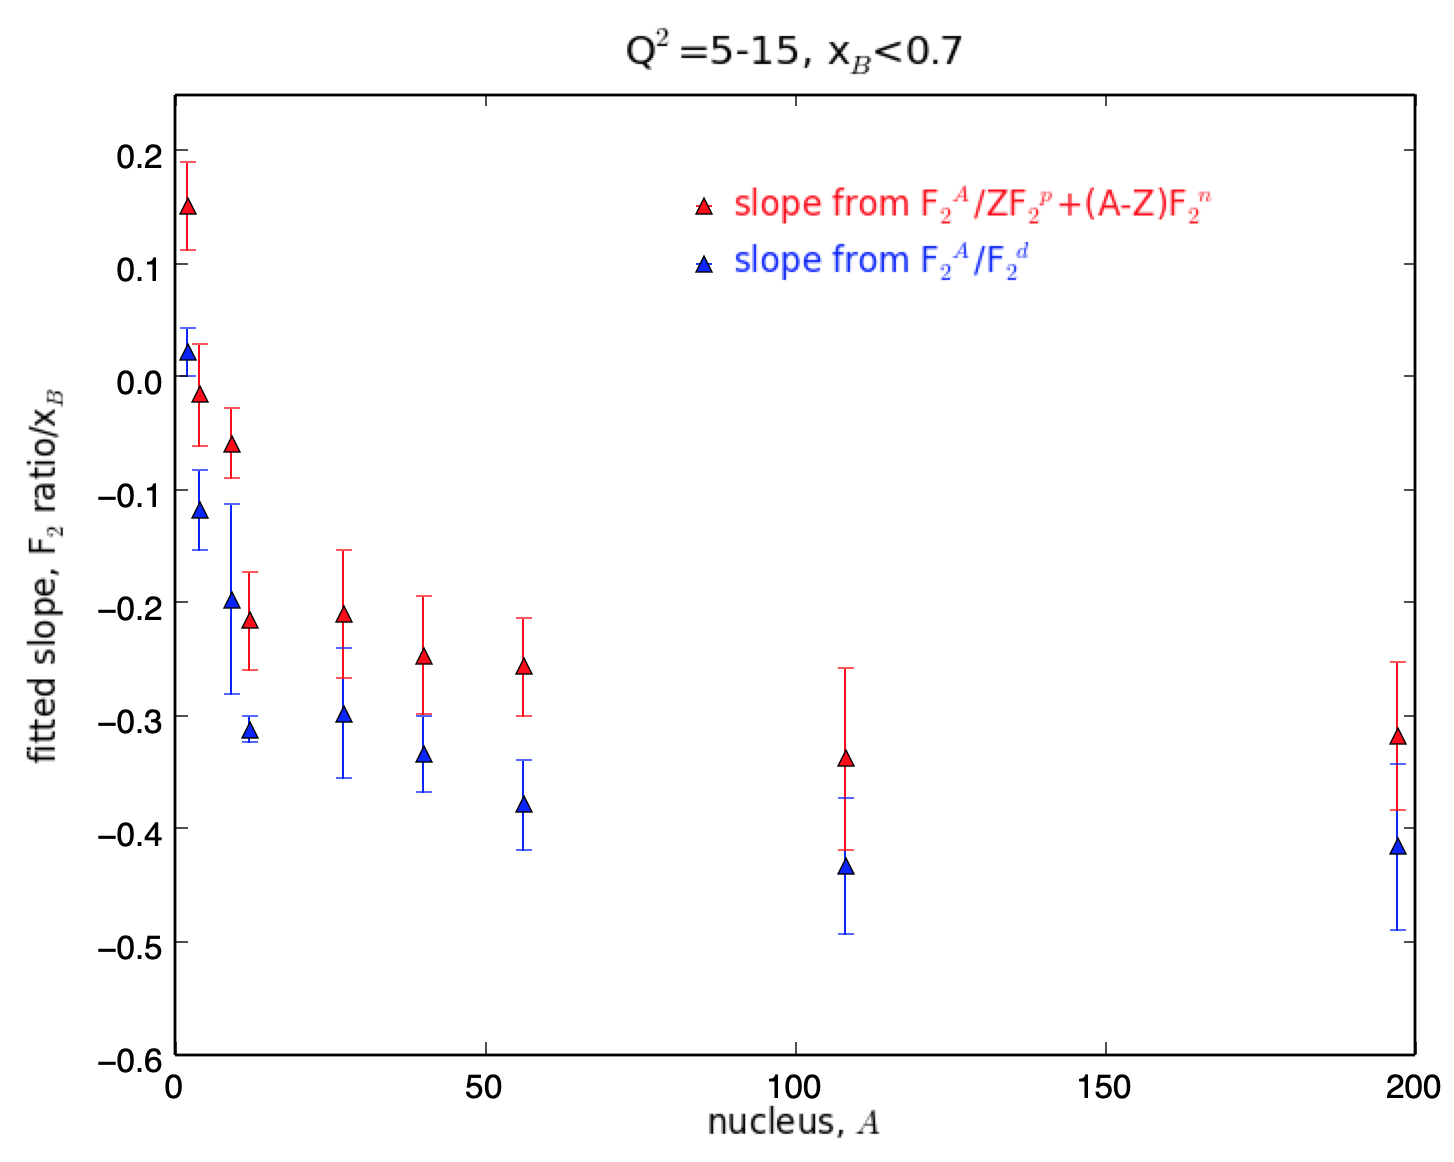
\includegraphics[width=\textwidth]{plots/plotsvA/Aslope_l7.png}
\end{minipage}\hfill\begin{minipage}{0.5\textwidth}
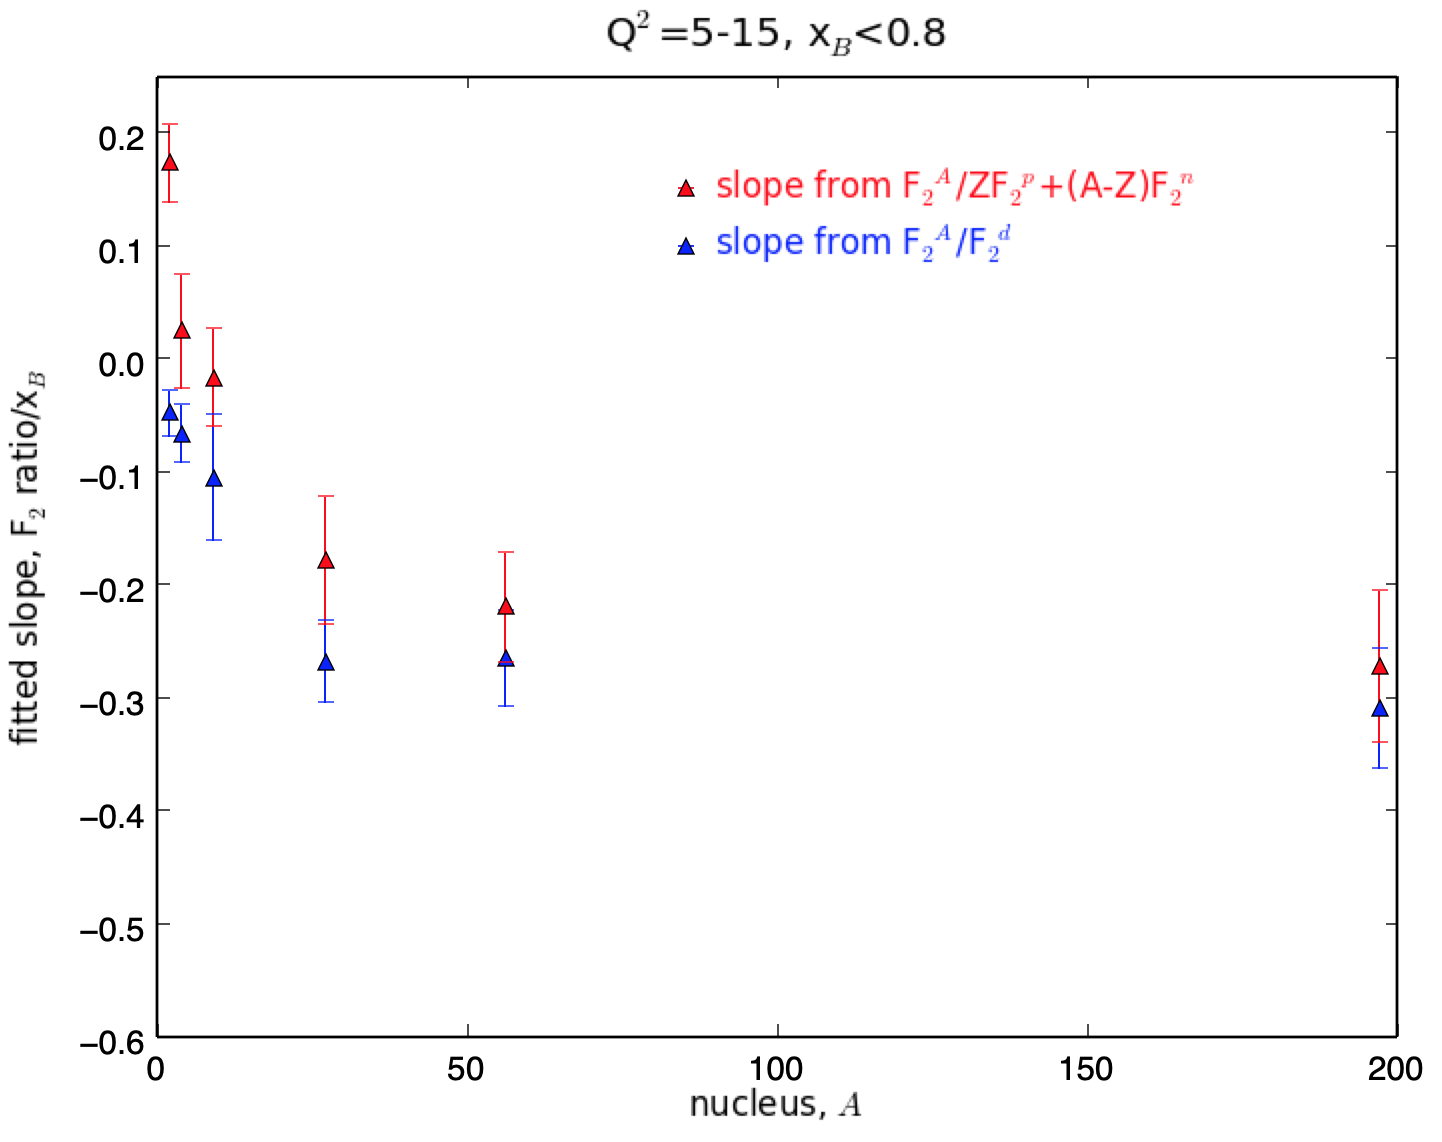
\includegraphics[width=\textwidth]{plots/plotsvA/Aslope_all.png}
\end{minipage}
  \caption[]{The slopes to the fits of the $F_2$ ratios versus $x_B$ are shown for both denominators and as a function of the nucleus $A$. In all cases,  the ratio taken with respect to the sum of the free neutron and free proton components exhibits a shallower slope than that taken deuterium.}
  \label{fig:Aslope_summary}
\end{figure}   

The slopes for each ratio for various cuts in $Q^2$ and $x_B$ are compared in Fig.~\ref{fig:Aslope_compare}. The inclusion of higher $Q^2$ and $x_B$ data in the fits generates slightly shallower slopes due to the rise seen from the nuclear effects. 

\begin{figure}[H]
\begin{minipage}{0.5\textwidth}
 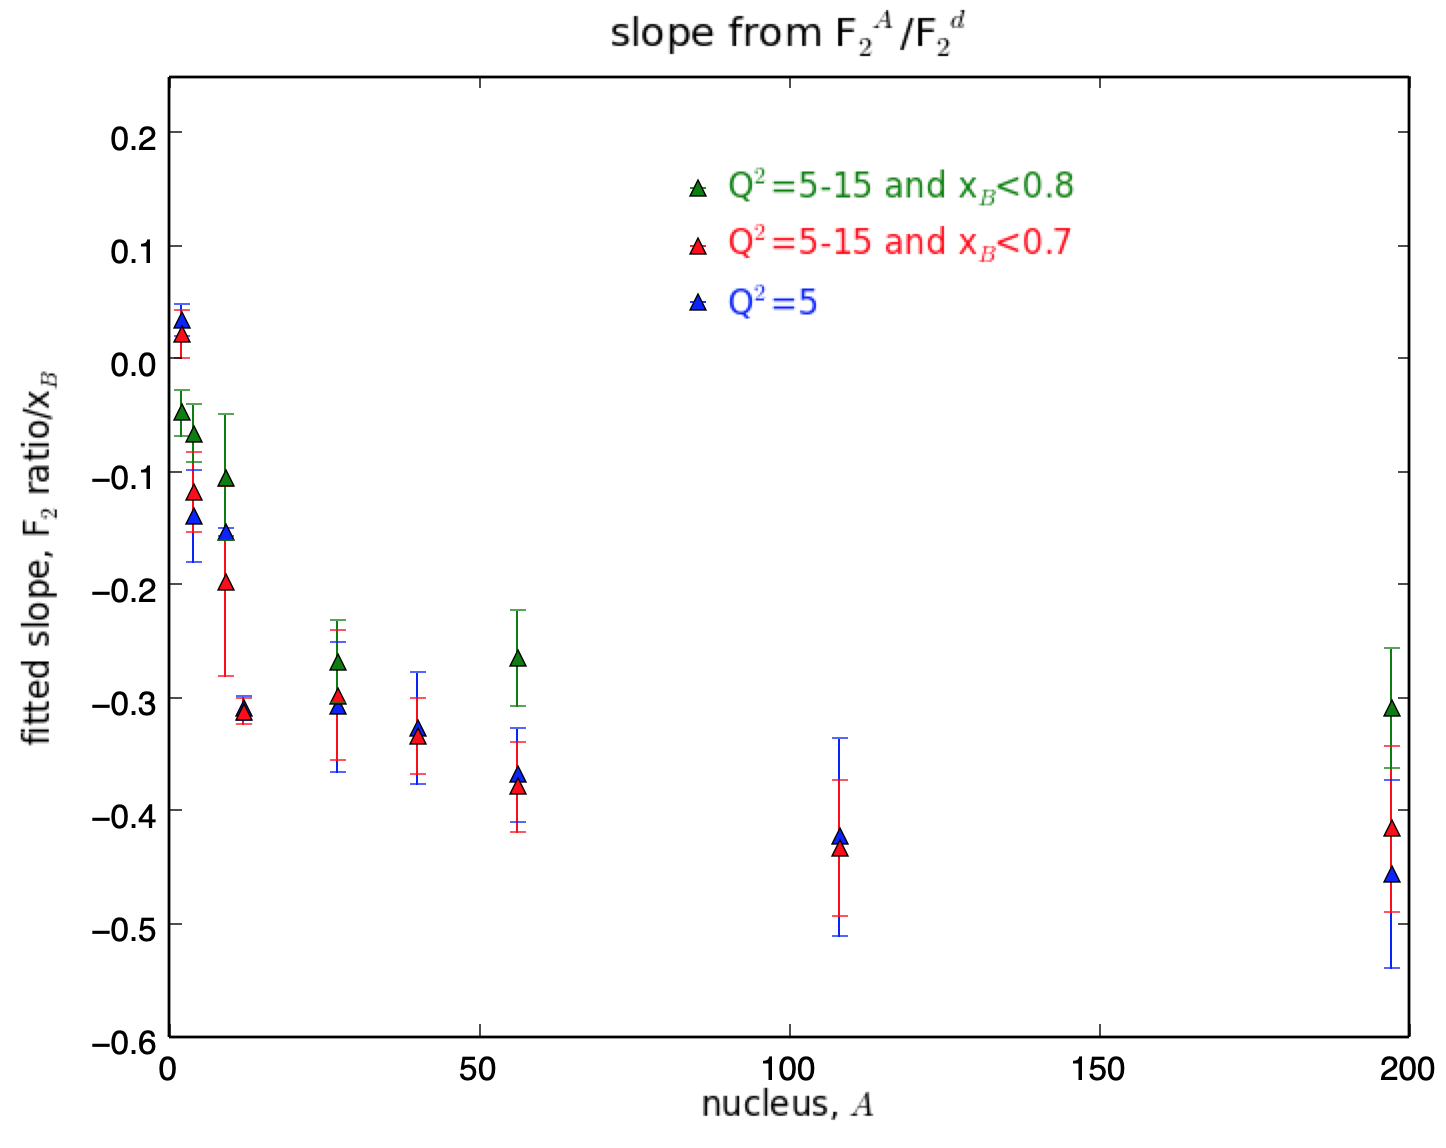
\includegraphics[width=\textwidth]{plots/plotsvA/Aslope_ad.png}
\end{minipage}\hfill\begin{minipage}{0.5\textwidth}
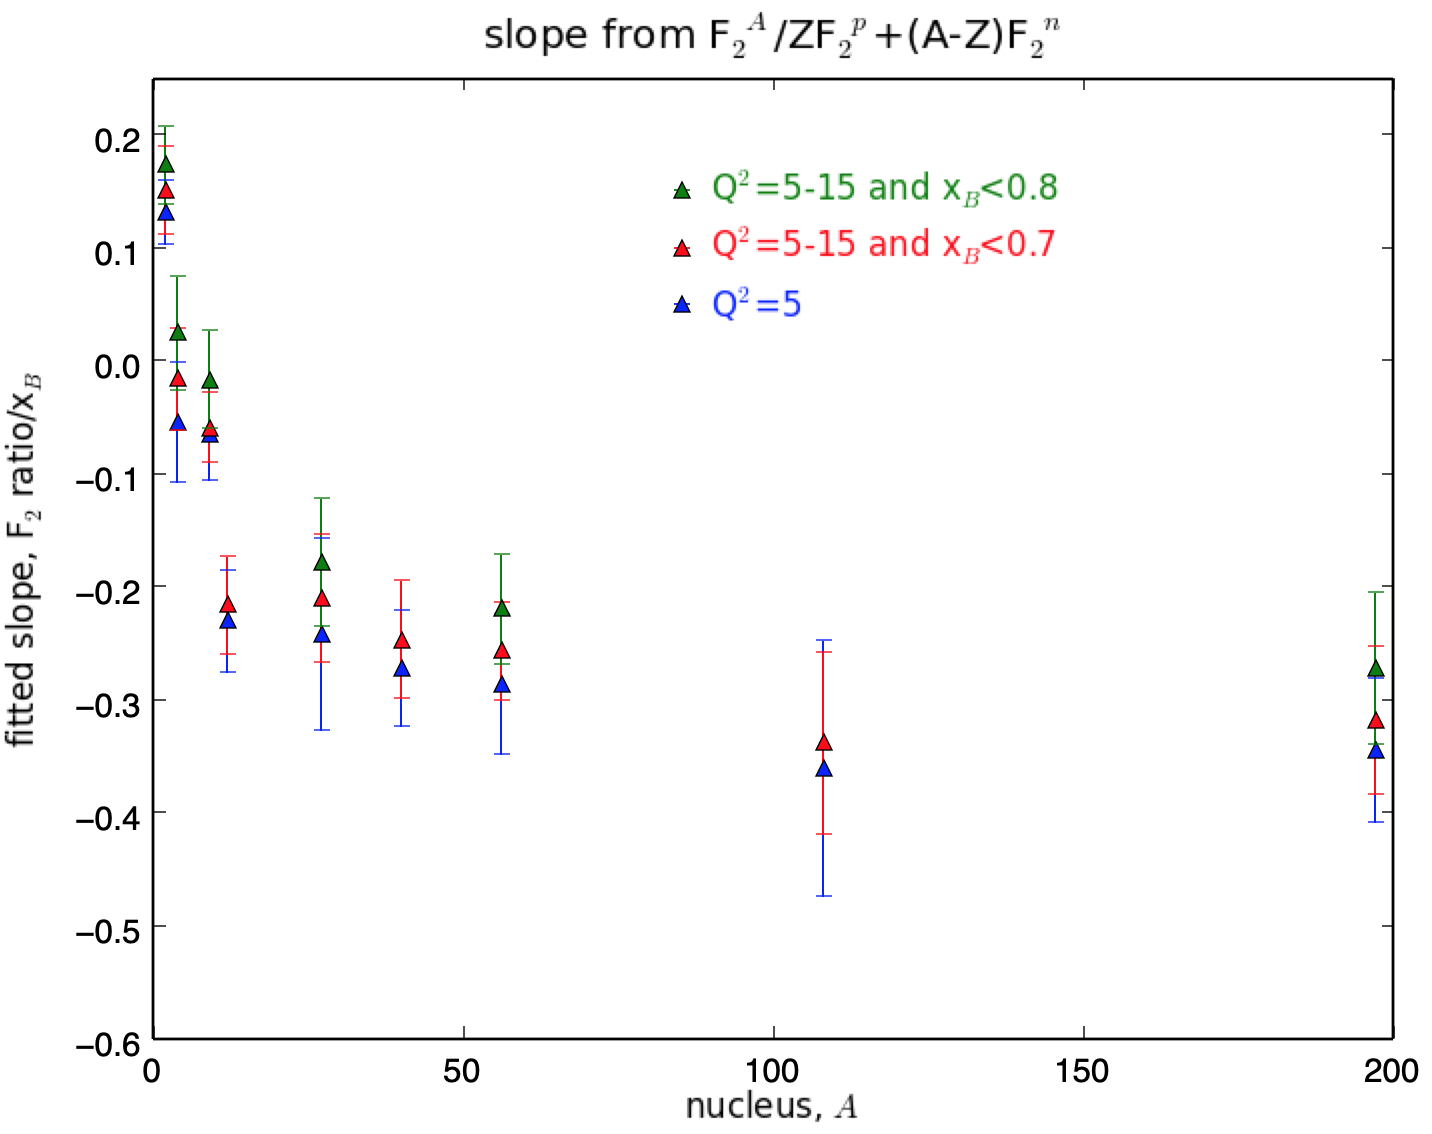
\includegraphics[width=\textwidth]{plots/plotsvA/Aslope_free.png}
\end{minipage}
  \caption[]{The slopes are compared for the different cuts in $Q^2$ and $x_B$. The inclusion of larger $Q^2$ and $x_B$ points in the fit generates a somewhat shallower slope.}
  \label{fig:Aslope_compare}
\end{figure}   

Table~\ref{SlopeFits} shows the fitted slope and intercept values for both the $F_2^A$ ratio for each nucleus taken with respect to deuterium and the sum of the free neutron and free proton contributions. In Table~\ref{SlopeFits}, only fits to the data where $Q^2=5$ are shown. No iso-scalar corrections are applied to the asymmetric nuclei.

\begin{table}[htb!]
\caption{\label{SlopeFits} Summary of linear fits to $x_B$ where $Q^2=5$.}
\centering
\begin{tabular}{ | C{2.5cm} | C{2cm} | C{2cm} | C{2cm} | C{2cm} | }
 \hline
 \textbf{Nucleus} & \textbf{A/d slope} & \textbf{A/d intercept} & \textbf{A/(n+p) slope} & \textbf{A/(n+p) intercept} \\ 
  \hline
deuterium & 0.034078+/-0.013514	& 0.963954+/-0.007694 & 0.131192+/-0.028952 &	0.893476+/-0.013877 \\ 
  \hline
  He4 & -0.139559+/-0.041514	 & 1.010444+/-0.023729 & -0.054561+/-0.053741 & 0.947196+/-0.027083 \\ 
 \hline
 Be & -0.153575+/-0.004225	 &1.020754+/-0.002375 &-0.064459+/-0.041653&	0.955925+/-0.020121\\ 
  \hline
   C & -0.310100+/-0.010935	& 1.081424+/-0.006245 & -0.230690+/-0.044742	&1.022234+/-0.022572  \\ 
  \hline
    Al &-0.308688+/-0.058075 &	1.074479+/-0.032618 & -0.241920+/-0.085474 &	1.021834+/-0.042052 \\ 
  \hline
 Ca &-0.327402+/-0.048885 &	1.085172+/-0.027035 & -0.27227+/-0.051774 &	1.037505+/-0.025103 \\ 
  \hline  
  Fe & -0.368335+/-0.041561&	1.085849+/-0.022646& -0.286425+/-0.062250 &	1.024809+/-0.029771 \\ 
  \hline 
  Ag & -0.423013+/-0.087616 &	1.119710+/-0.048607 & -0.360732+/-0.113255	& 1.068858+/-0.055132 \\ 
  \hline 
   Au & -0.456231+/-0.083041	&1.098650+/-0.045601 & -0.344872+/-0.063026 &	1.023289+/-0.030740\\ 
  \hline 
    \end{tabular}
\end{table} 

Table~\ref{SlopeFits1} shows the fitted slope and intercept values for both the $F_2^A$ ratios where all E139 $Q^2$ data are included at $x_B<0.7.$ 

\begin{table}[htb!]
\caption{\label{SlopeFits1} Summary of linear fits to $x_B$ where $Q^2=5-15$ and $x_B<0.7$.}
\centering
\begin{tabular}{ | C{2.5cm} | C{2cm} | C{2cm} | C{2cm} | C{2cm} | }
 \hline
 \textbf{Nucleus} & \textbf{A/d slope} & \textbf{A/d intercept} & \textbf{A/(n+p) slope} & \textbf{A/(n+p) intercept} \\ 
  \hline
deuterium & 0.021260+/-0.020875 &	0.974781+/-0.011910 & 0.150795+/-0.039755	& 0.894508+/-0.019402 \\ 
  \hline
  He4 &-0.118090+/-0.035769 &	0.997067+/-0.020596 & -0.016222+/-0.045129 &	0.931353+/-0.023103 \\ 
 \hline
 Be &-0.197454+/-0.083778 &	1.035493+/-0.048067 &-0.059106+/-0.030303 &	0.953386+/-0.015144\\ 
  \hline
   C &-0.312985+/-0.011614	&1.082614+/-0.006717 & -0.216581+/-0.043641	&1.016811+/-0.022474 \\ 
  \hline
    Al &-0.298244+/-0.057500	&1.070859+/-0.032829 & -0.210889+/-0.056564	&1.010775+/-0.028368 \\ 
  \hline
 Ca &-0.334267+/-0.034303&	1.088128+/-0.019560 & -0.247045+/-0.051788 &	1.027656+/-0.025990 \\ 
  \hline  
  Fe & -0.379082+/-0.040058	&1.085956+/-0.022621& -0.257315+/-0.043599 &	1.010276+/-0.021402 \\ 
  \hline 
  Ag &-0.432939+/-0.060259&	1.124006+/-0.034442 & -0.338549+/-0.081071	&1.060178+/-0.040839 \\ 
  \hline 
   Au & -0.416652+/-0.073092&	1.076493+/-0.041418 & -0.318705+/-0.065007&	1.012124+/-0.032502\\ 
  \hline 
    \end{tabular}
\end{table} 

Table~\ref{SlopeFits2} shows the fitted slope and intercept values for both the $F_2^A$ ratios where all E139 $Q^2$ data are included with no cuts on $x_B$. 


\begin{table}[htb!]
\caption{\label{SlopeFits2} Summary of linear fits to $x_B$ where $Q^2=5-15$ and $x_B<0.8$.}
\centering
\begin{tabular}{ | C{2.5cm} | C{2cm} | C{2cm} | C{2cm} | C{2cm} | }
 \hline
 \textbf{Nucleus} & \textbf{A/d slope} & \textbf{A/d intercept} & \textbf{A/(n+p) slope} & \textbf{A/(n+p) intercept} \\ 
  \hline
deuterium & -0.047904+/-0.020441	&1.011339+/-0.013123& 0.173649+/-0.034450	&0.885021+/-0.017643 \\ 
  \hline
  He4 &-0.066610+/-0.025529&	0.969128+/-0.015975 & 0.024671+/-0.050676&	0.913125+/-0.026599 \\ 
 \hline
 Be &-0.105347+/-0.056027&	0.986067+/-0.035211 &-0.016830+/-0.042937&	0.934997+/-0.022080\\ 
  \hline
   C &---&--- & ---	&--- \\ 
  \hline
    Al &-0.268256+/-0.036285	&1.054884+/-0.022384&-0.178675+/-0.057032&	0.996550+/-0.029163 \\ 
  \hline
 Ca &---&--- & ---	&--- \\ 
  \hline  
  Fe &-0.265522+/-0.041894	&1.026296+/-0.025600&-0.219929+/-0.048613	&0.994104+/-0.024310\\ 
  \hline 
  Ag &---&--- & ---	&---  \\ 
  \hline 
   Au & -0.309382+/-0.053346 &	1.019493+/-0.032947 & -0.272132+/-0.066892 &	0.991273+/-0.034131\\ 
  \hline 
    \end{tabular}
\end{table} 

The slopes from Table~\ref{SlopeFits} where $Q^2=5$ only are shown plotted against the SRC factor, $a_2$. The general fitted slope is still linear across the $a_2$ values for each nucleus, but there is a clear systematic offset between the intercept values of these two fits. The fits to the slopes with respect to the SRC factor are shown in Fig.~\ref{fig:a2_src}.

\begin{figure}[H]
\begin{minipage}{0.5\textwidth}
      	  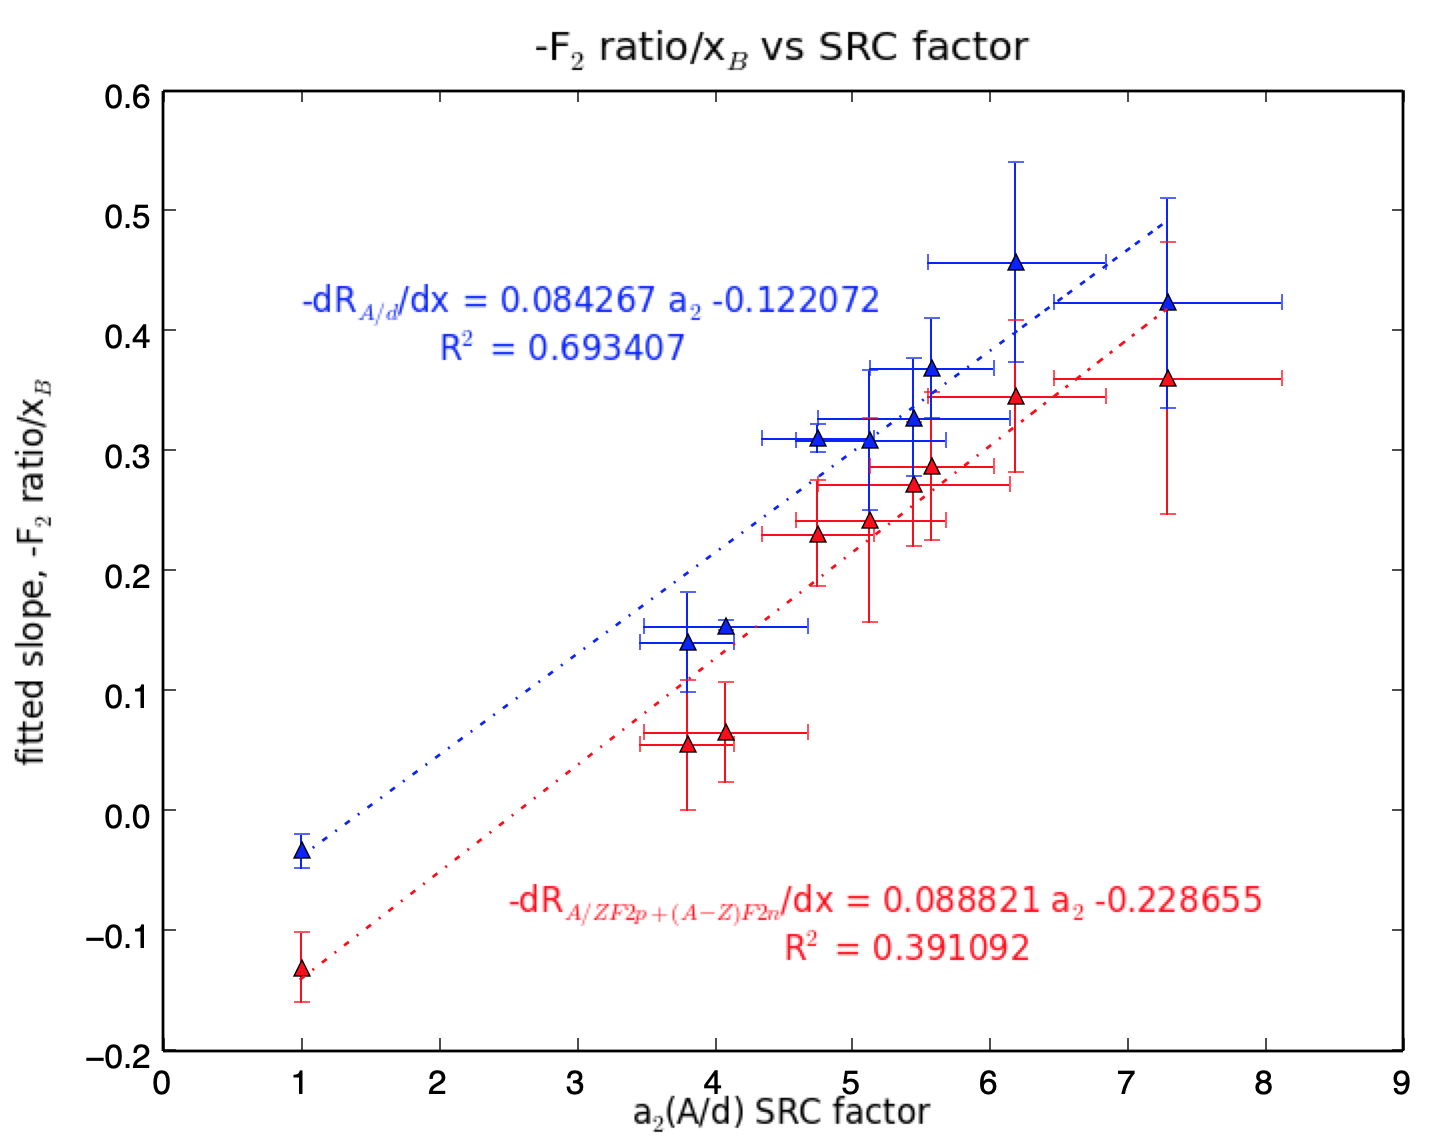
\includegraphics[width=\textwidth]{plots/a2SRC.png}
      	  \end{minipage}\hfill\begin{minipage}{0.5\textwidth}
      	        	  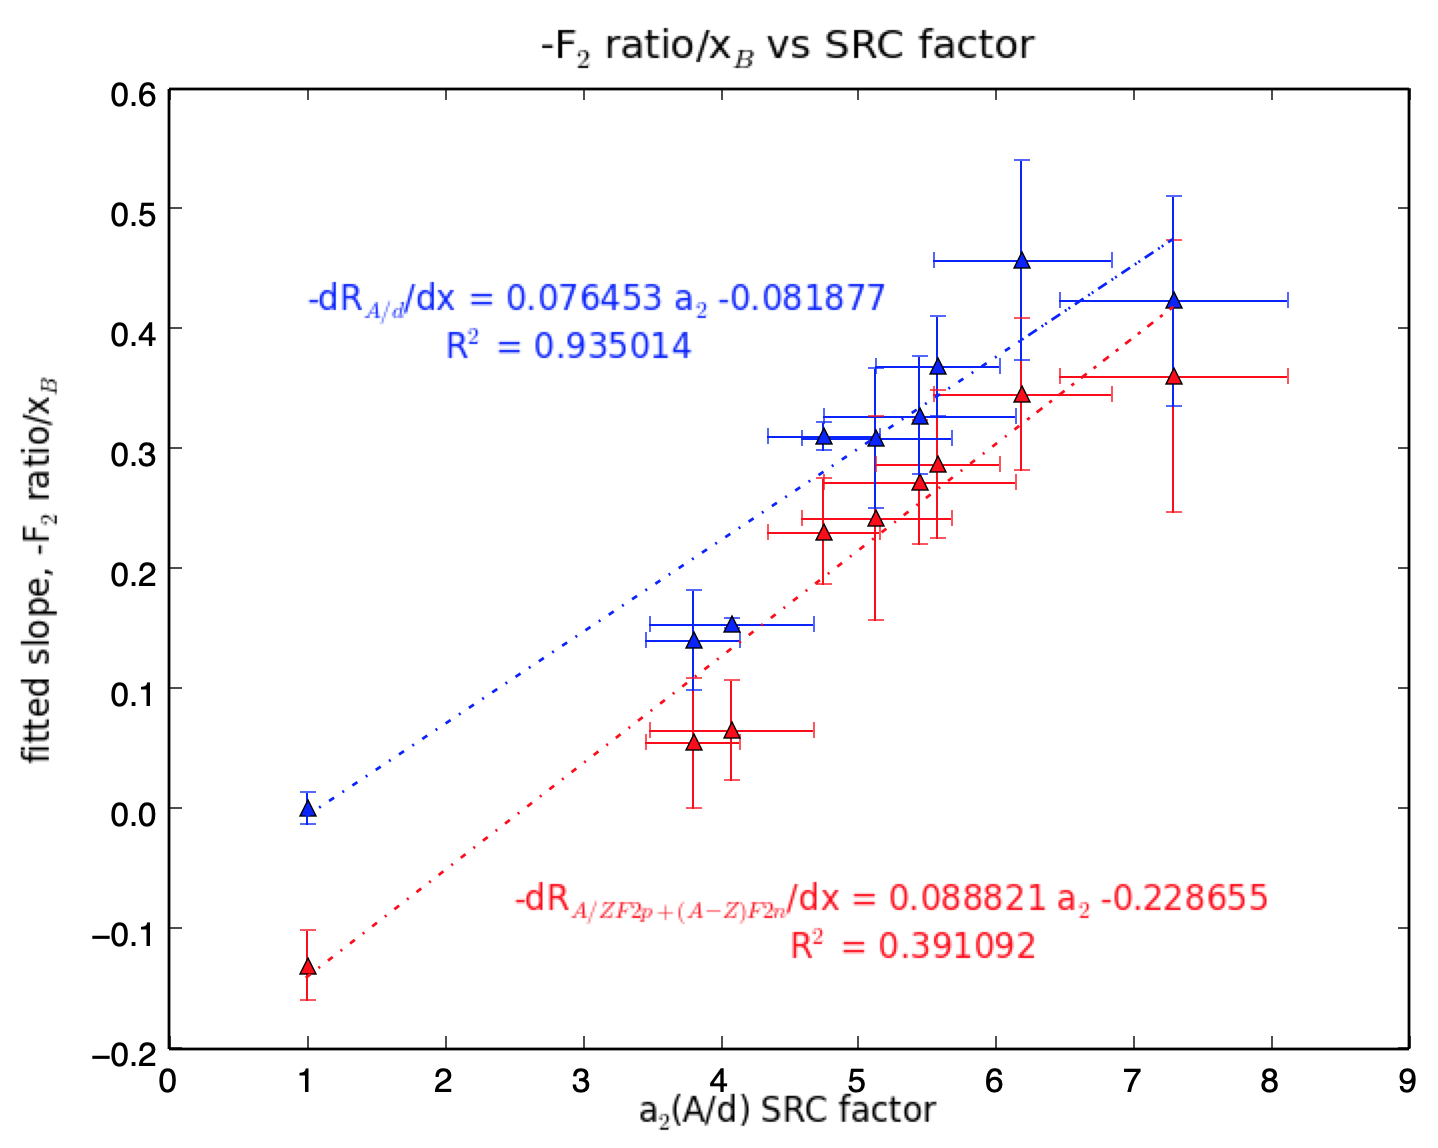
\includegraphics[width=\textwidth]{plots/a2SRCfixed.png}
\end{minipage}
 	 \caption[]{The slopes fit to the data for $Q^2=5$ are shown versus the $a_2$ SRC factor. Left: The slope value for deuterium is that which was obtained from the fits and corresponds to Table~\ref{SlopeFits}. Right: The slope value for deuterium is set to 0.}
  \label{fig:a2_src}
 \end{figure}
 
The intercept value of approximately -0.08 for the ratio taken with respect to deuterium when the deuterium point is set to 0 (Fig.~\ref{fig:a2_src} right) is consistent with previous studies. The intercept value is significantly smaller for the data where the original slope ratio was taken with respect to the sum of the free proton and free neutron contributions. 

\section{Conclusions}

The CJ Collaboration has recently extracted the free neutron structure function from the world DIS data opening new windows for exploring the EMC Effect and deuteron nuclear effects. General observations show that the deuteron ratio to the sum of the free proton and free neutron structure functions has some dependencies with $Q^2$. These dependencies have been generally ignored by previous experiments. The changes with $Q^2$ are most significant at large $Q^2$ and large $x_B$. As the EMC Effect is calculated from the slope of the nucleus to deuteron structure function ratio, there is an apparent contamination of these results due to the nuclear effects of the deuteron alone. Additionally, these effects imply that the structure function ratios at $x_B>0.6$ do not follow the linear trend of the data where $x_B$ is $>0.3$ and $x_B<0.6$.Therefore, it would seem that the EMC Effect as calculated using the slope of the $F_2^A/F_2^d$ ratio has and $x_B$ and $Q^2$ dependence. Also, there appears to be a more significant spread in $A$ in the data where the the structure function of the nucleus is taken with respect to the neutron vs the proton. This spread arises from the drop in the ratio $F_2^n/F_2^p$ as a function of $x_B$. 

\section{Acknowledgments}

The authors would like to thank Shujie Li for constructing the most complete world $F_2^n$ data set to date and Alberto Accardi and Wally Melnitchouk for providing crucial insights and interpretations for this analysis.  

%----------------------------------------------------------------------------------------
%	REFERENCE LIST
%----------------------------------------------------------------------------------------

\begin{thebibliography}{99} 

\bibitem{CJ15Fit} A. Accardi, L. T. Brady, W. Melnitchouk, J. F. Owens and N. Sato, Phys.Rev. D93 (2016) 114017

\bibitem{Gomez:1993ri} 
  J.~Gomez {\it et al.},
  ``Measurement of the A-dependence of deep inelastic electron scattering,''
  Phys.\ Rev.\ D {\bf 49}, 4348 (1994).
  doi:10.1103/PhysRevD.49.4348

\bibitem{Griffioen:2015hxa} 
  K.~A.~Griffioen {\it et al.},
  ``Measurement of the EMC Effect in the Deuteron,''
  Phys.\ Rev.\ C {\bf 92}, no. 1, 015211 (2015)
  doi:10.1103/PhysRevC.92.015211
  [arXiv:1506.00871 [hep-ph]].

\bibitem{Rubin:2011} 
  J.~G.~Rubin, J.~Arrington,
  ``A New Extraction of Neutron Structure Functions from Existing Inclusive DIS Data,''
  doi:	10.1063/1.3631528
  [arXiv:1101.3506v2 [nucl-ex]].
  
\bibitem{Whitlow:R1990} L.W.Whitlow, SLAC-Report-357, Ph.D. Thesis, Stanford University, March 1990.

\bibitem{XS_E139} https://www.slac.stanford.edu/exp/e139/E139.RESULTS

\bibitem{XS_d} http://www.slac.stanford.edu/exp/e140/SIGMA.D2\_357

\bibitem{KulaginPetti} Alekhin, S. I. and Kulagin, S. A. and Petti, R.,
  ``Nuclear effects in the deuteron and constraints on the $d/u$ ratio,''
  Phys.\ Rev.\ D {\bf 96}, no. 5, 0054005 (2017)
  doi:10.1103/PhysRevD.96.054005
  [arXiv:1704.00204].

\bibitem{Malace:2014uea} 
  S.~Malace, D.~Gaskell, D.~W.~Higinbotham and I.~Cloet,
  ``The Challenge of the EMC Effect: existing data and future directions,''
  Int.\ J.\ Mod.\ Phys.\ E {\bf 23}, no. 08, 1430013 (2014)
  doi:10.1142/S0218301314300136
  [arXiv:1405.1270 [nucl-ex]].
 
 
\end{thebibliography}

%----------------------------------------------------------------------------------------

%\begin{description}
%\item[$\bullet$ Version 1] Applied on December 11, 2017 at 4:21~am starting with SHMS run 1605. All quads are scaled by a factor of 1.05 times their nominal setting. The HB and dipole are not modified~\cite{V1_holly}.
%\item[$\bullet$ Version 2] Applied on December 19, 2017 at 9:06~am starting with SHMS run 1655. The original 1.05 scale factor for the quads is removed and modified to be: Q1 at 1.03, Q2 at 1.04, Q3 at 1.03~\cite{V2_holly}.
%\item[$\bullet$ Version 3] Applied on April 5, 2018 at 3:47~pm starting with coincidence run 3288. The Q1 and Q3 saturation modifications (in the code) are completely removed~\cite{V3_holly}.
%\item[$\bullet$ Version 4 and 5] Applied on August 14, 2018 at 6:14~pm starting with SHMS run 4432, HMS run 2347, and coincidence run 4436. All SHMS magnets (HB, Q1, Q2, Q3, dipole) and scaled up by a factor of 1/0.983 from the commissioning studies in order to better match the desired central momentum setting~\cite{V4_holly}. Additionally, any non-linear dipole modeling behavior is removed. 
%\item[$\bullet$ Version 6] Applied on September 29, 2018 at 5:06~pm starting with coincidence run 4780. A saturation model for Q1 is applied at 6~GeV and above: $1/(-0.00077P^2+0.0132P+0.94938)$. This was not studied above 8.035~GeV central momentum and uses a constant value at and above 8.035~GeV from the equation. 
%\end{description}

\section{Appendix}
\begin{figure}[H]
\begin{minipage}{0.5\textwidth}
 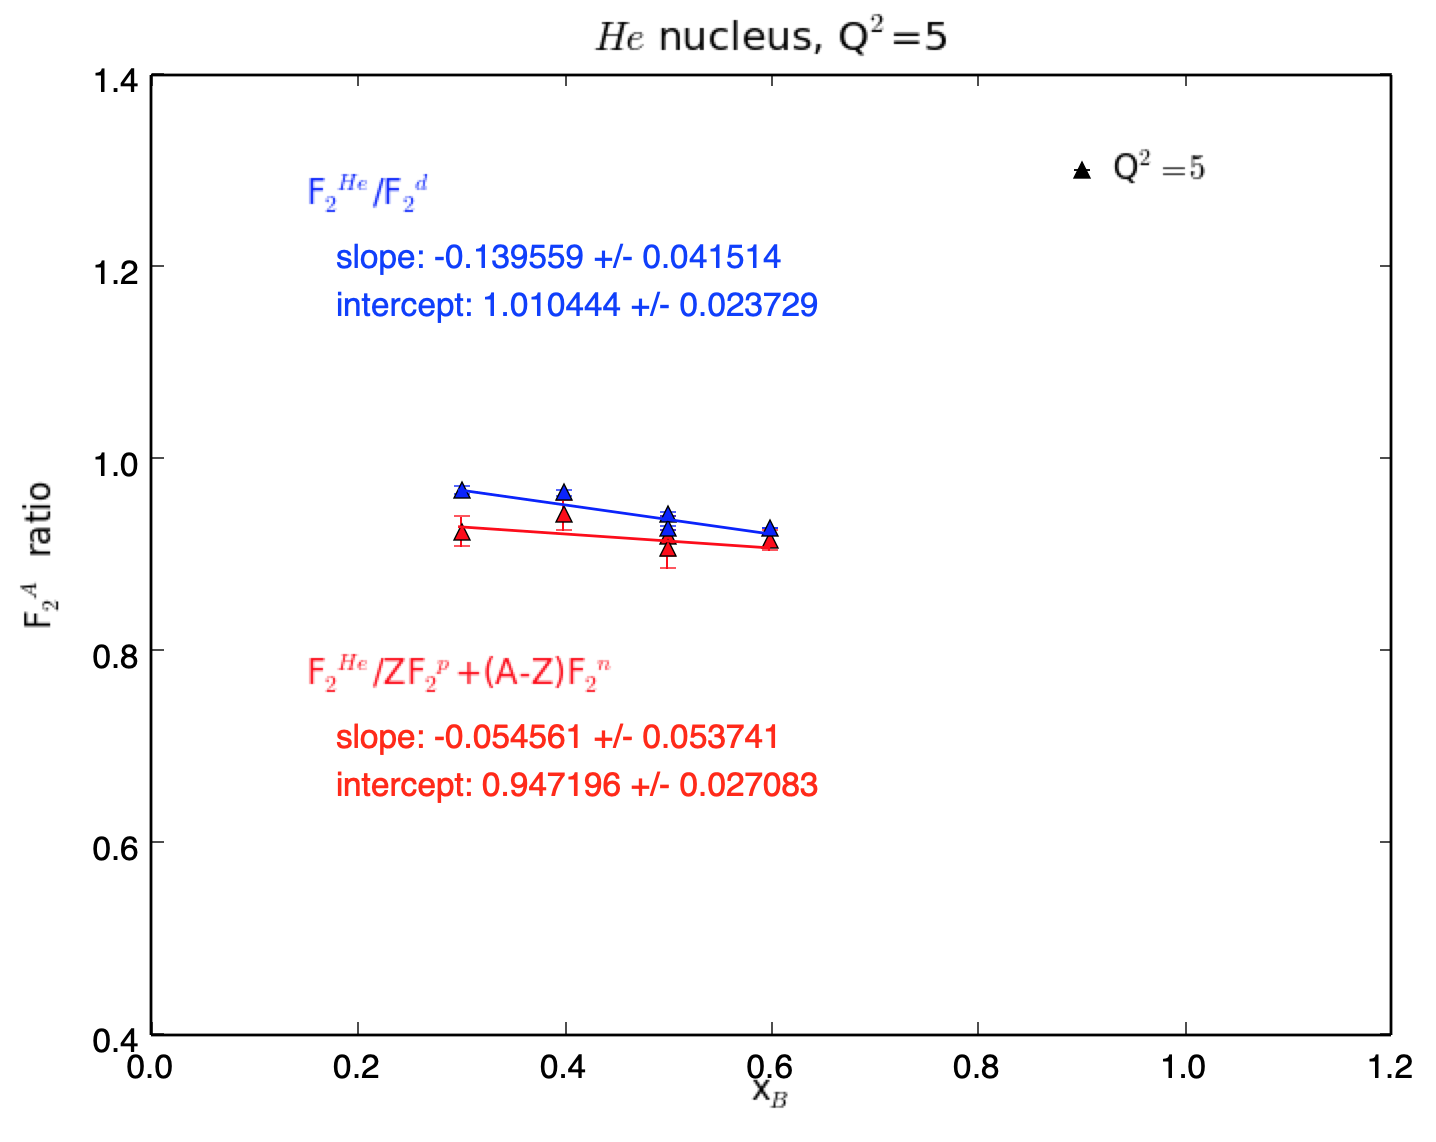
\includegraphics[width=\textwidth]{plots/q2_5/q2_5_He.png}
\end{minipage}\hfill\begin{minipage}{0.5\textwidth}
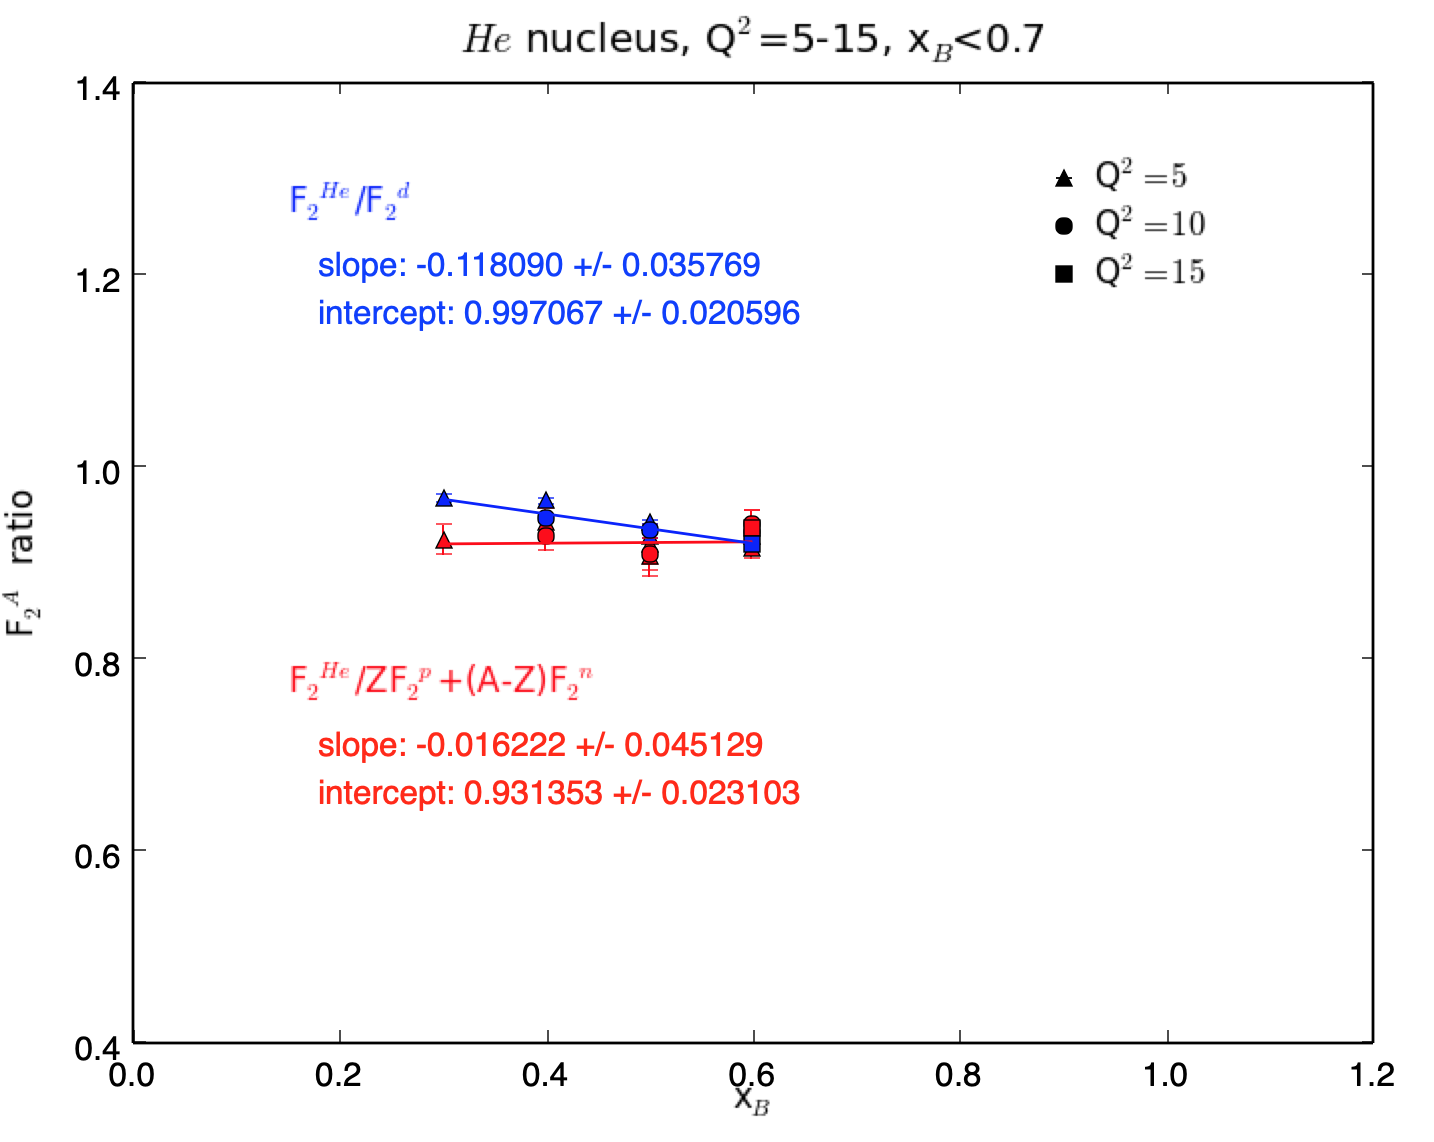
\includegraphics[width=\textwidth]{plots/q2_all_x_l7/q2_all_x_l7_He.png}
\end{minipage}\hfill\begin{minipage}{0.5\textwidth}
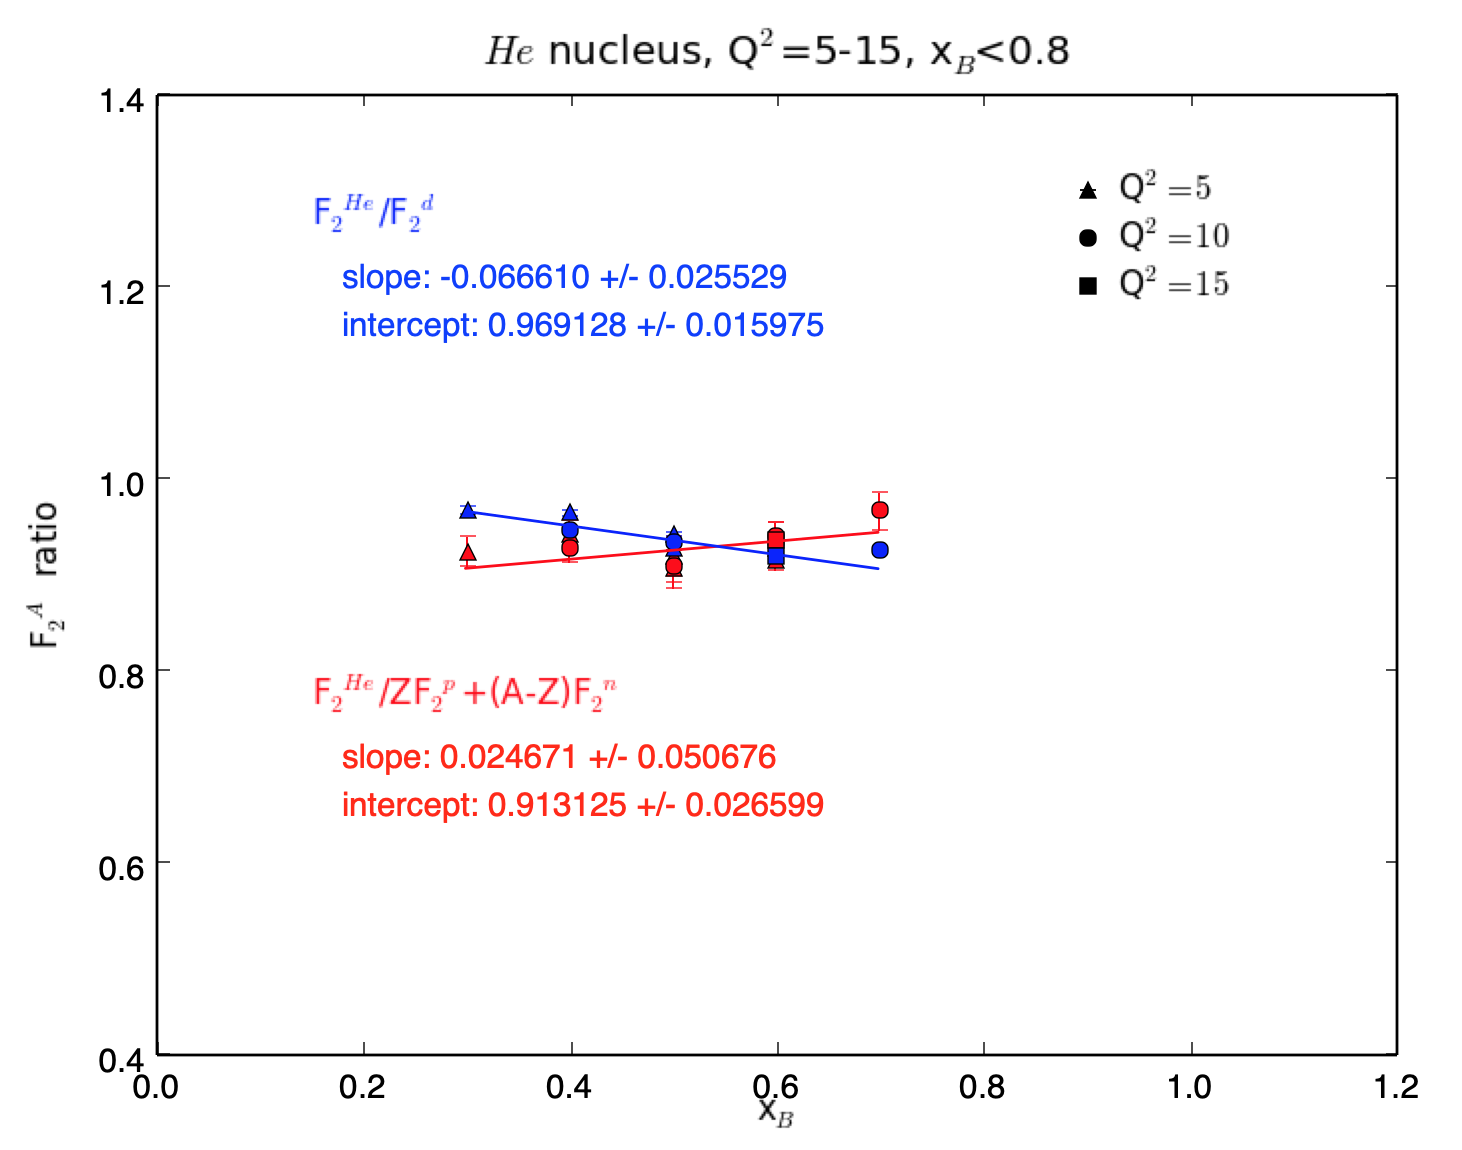
\includegraphics[width=\textwidth]{plots/q2_all_x_all/all_He.png}
\end{minipage}
  \caption[]{Linear fits to the $He$ target data with cuts on $Q^2$ and $x_B$.}
  \label{fig:fits_He}
\end{figure}   

 \begin{figure}[H]
\begin{minipage}{0.5\textwidth}
 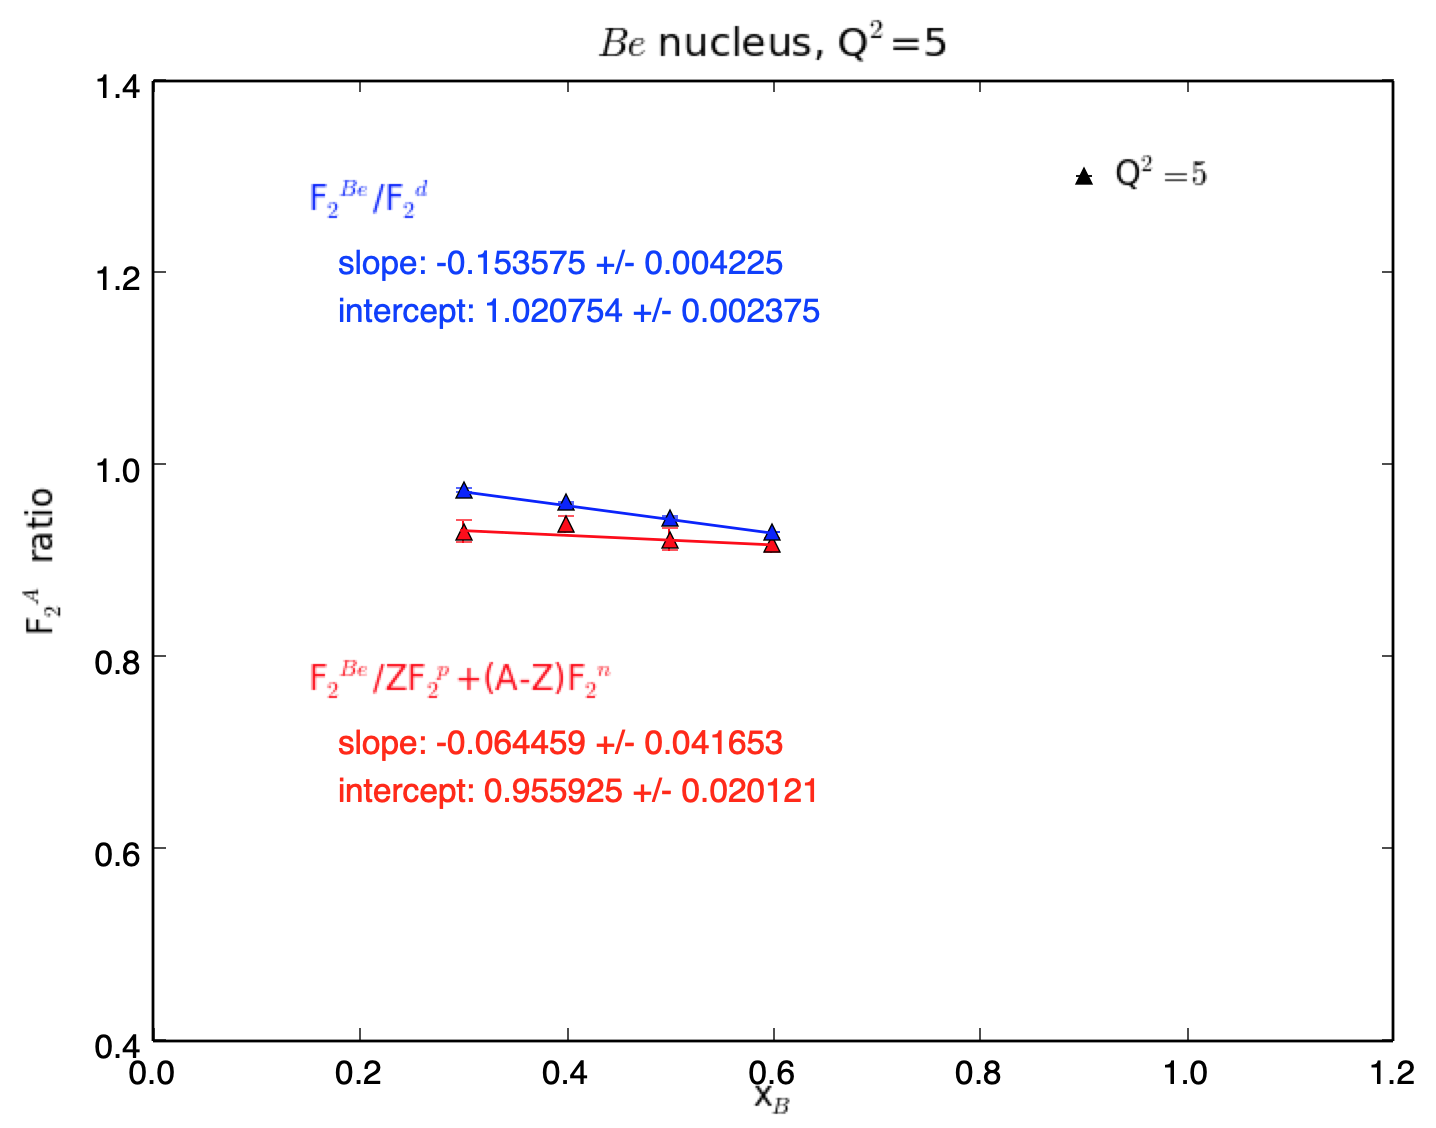
\includegraphics[width=\textwidth]{plots/q2_5/q2_5_Be.png}
\end{minipage}\hfill\begin{minipage}{0.5\textwidth}
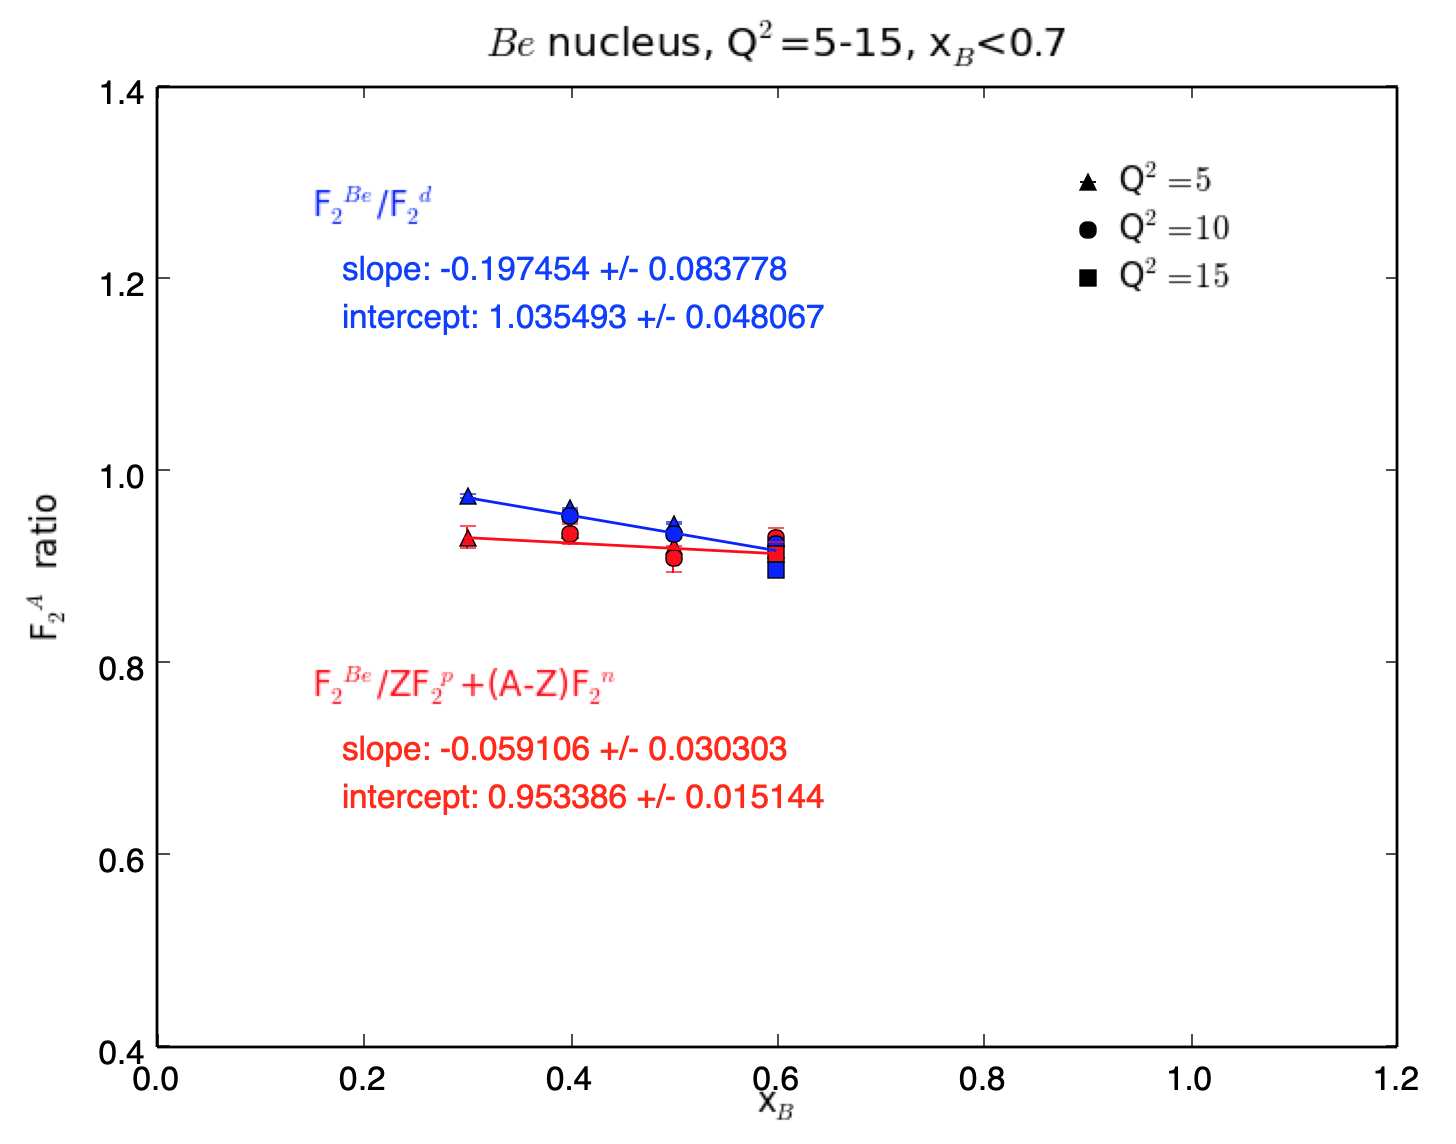
\includegraphics[width=\textwidth]{plots/q2_all_x_l7/q2_all_x_l7_Be.png}
\end{minipage}\hfill\begin{minipage}{0.5\textwidth}
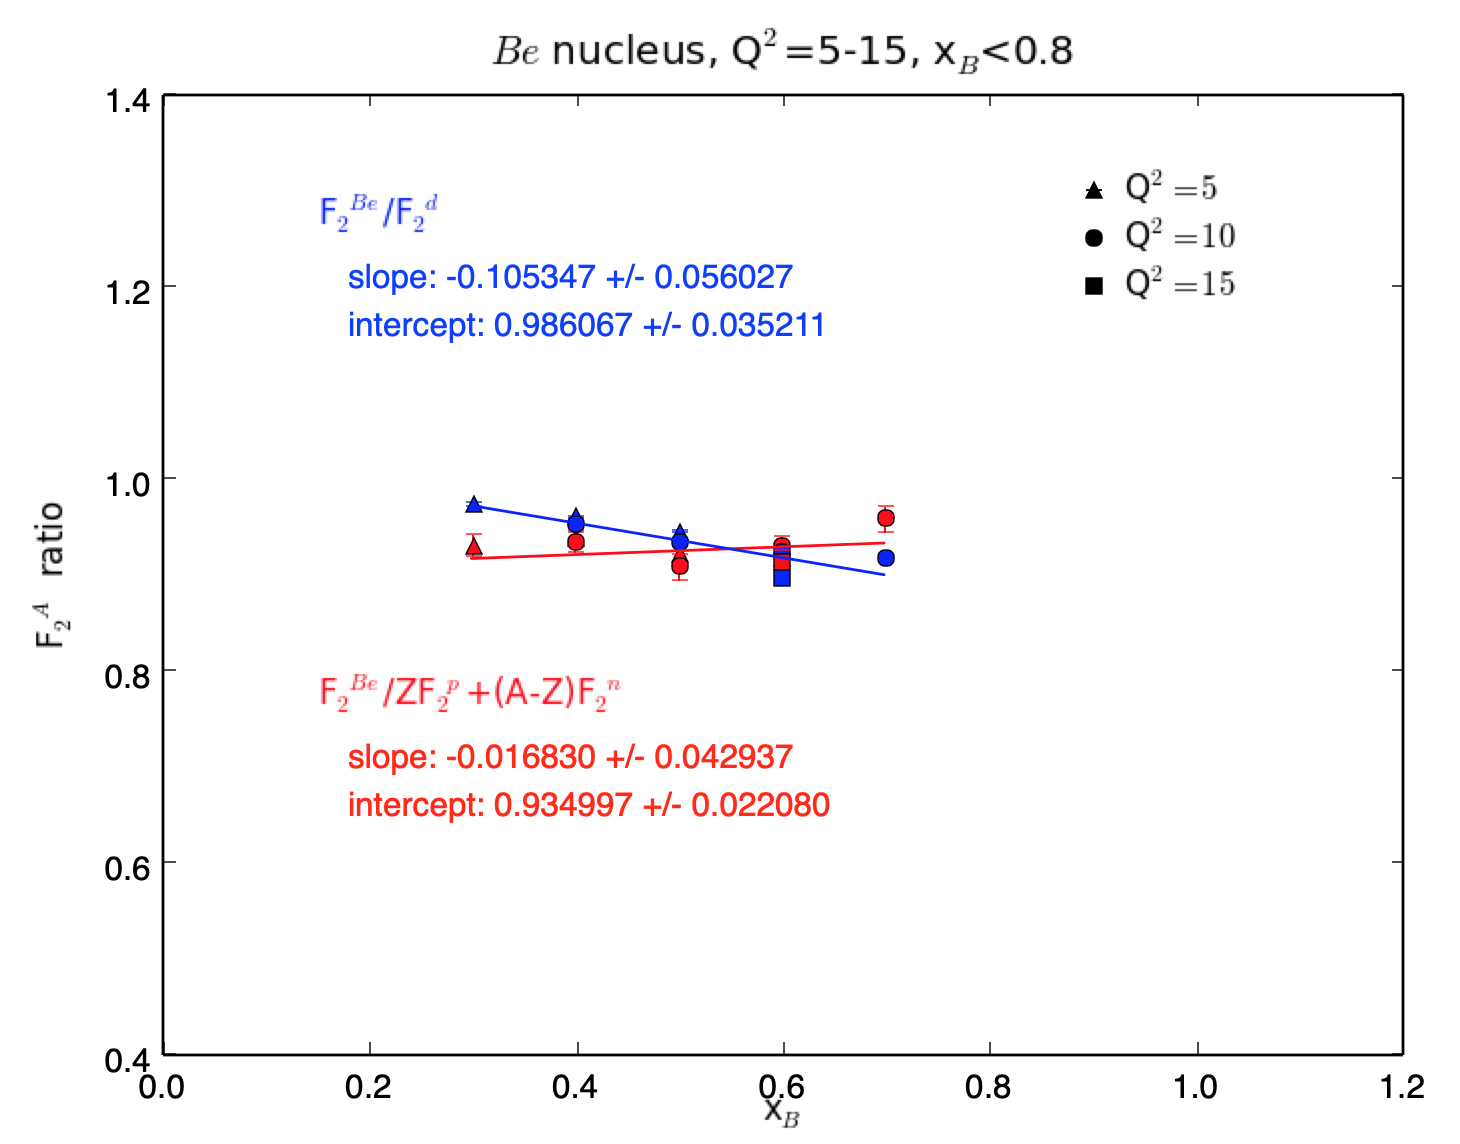
\includegraphics[width=\textwidth]{plots/q2_all_x_all/all_Be.png}
\end{minipage}
  \caption[]{Linear fits to the $Be$ target data with cuts on $Q^2$ and $x_B$.}
  \label{fig:fits_Be}
\end{figure}   


 \begin{figure}[H]
\begin{minipage}{0.5\textwidth}
 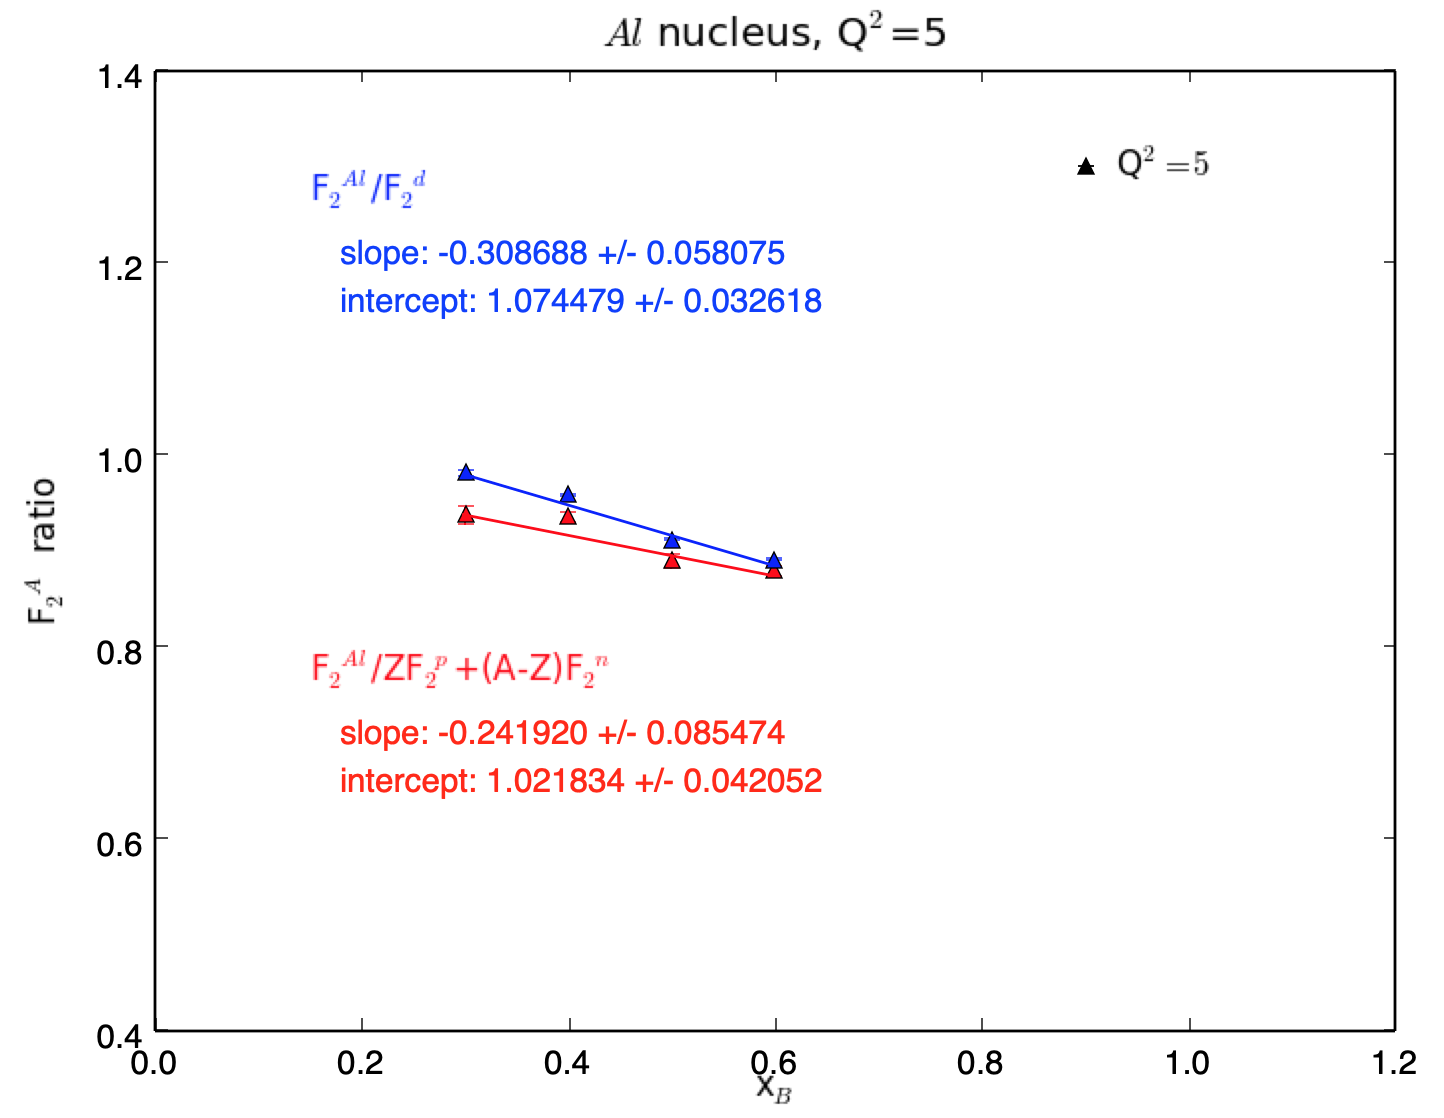
\includegraphics[width=\textwidth]{plots/q2_5/q2_5_Al.png}
\end{minipage}\hfill\begin{minipage}{0.5\textwidth}
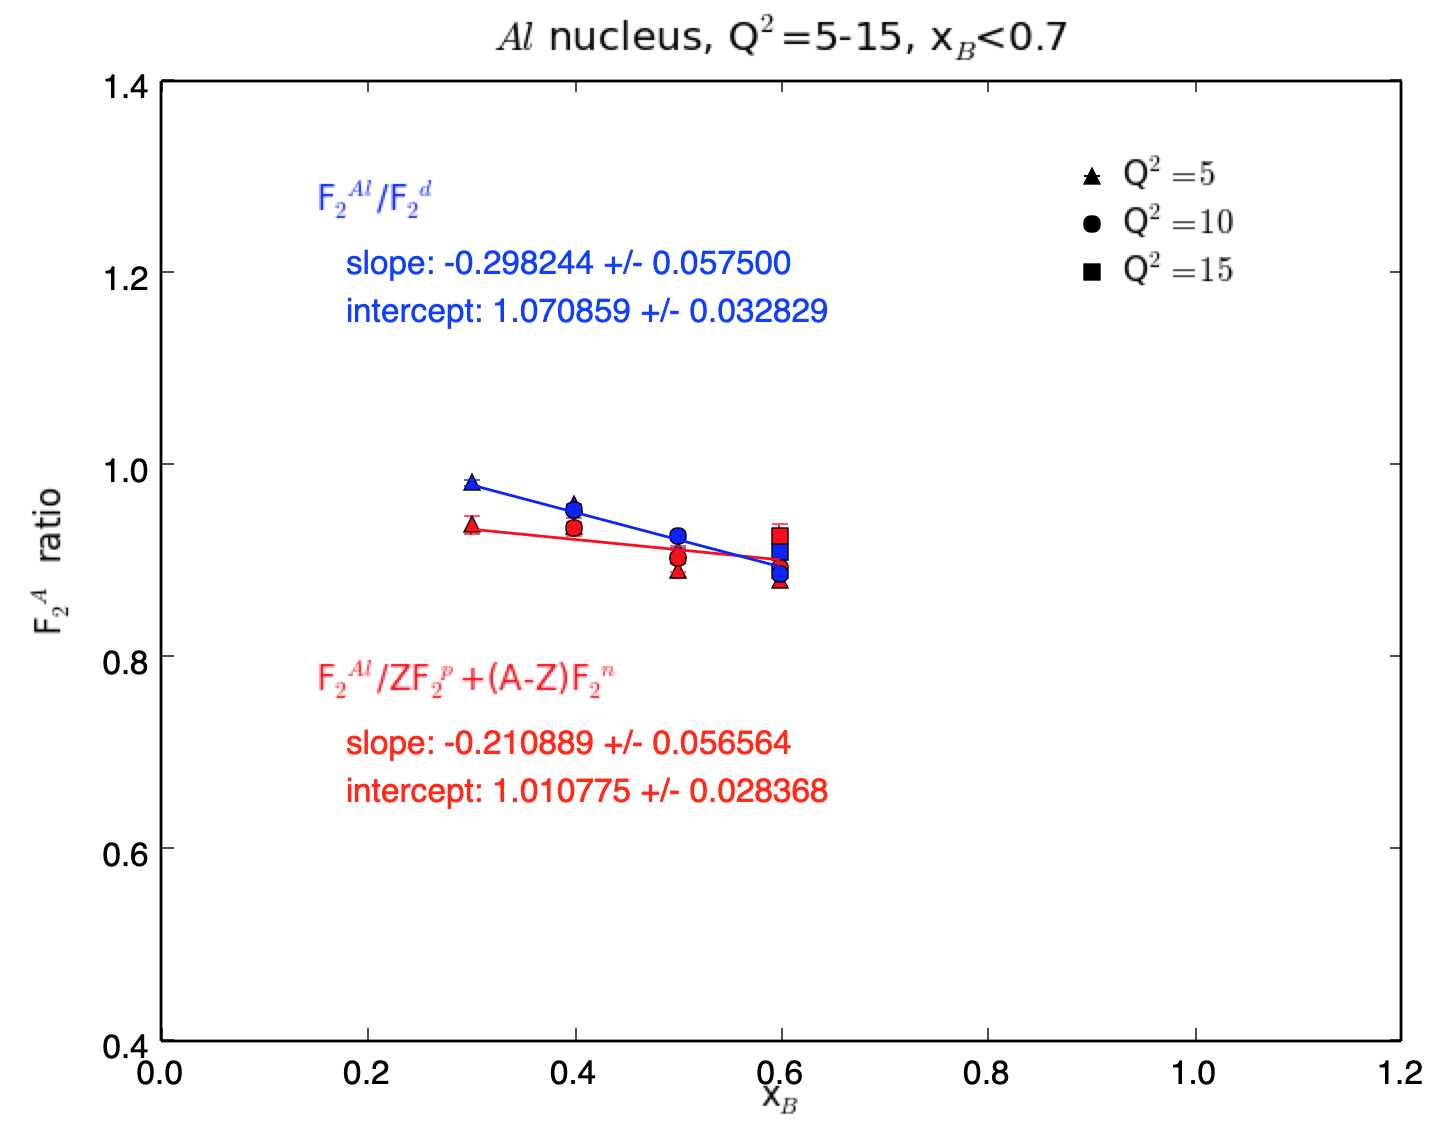
\includegraphics[width=\textwidth]{plots/q2_all_x_l7/q2_all_x_l7_Al.png}
\end{minipage}\hfill\begin{minipage}{0.5\textwidth}
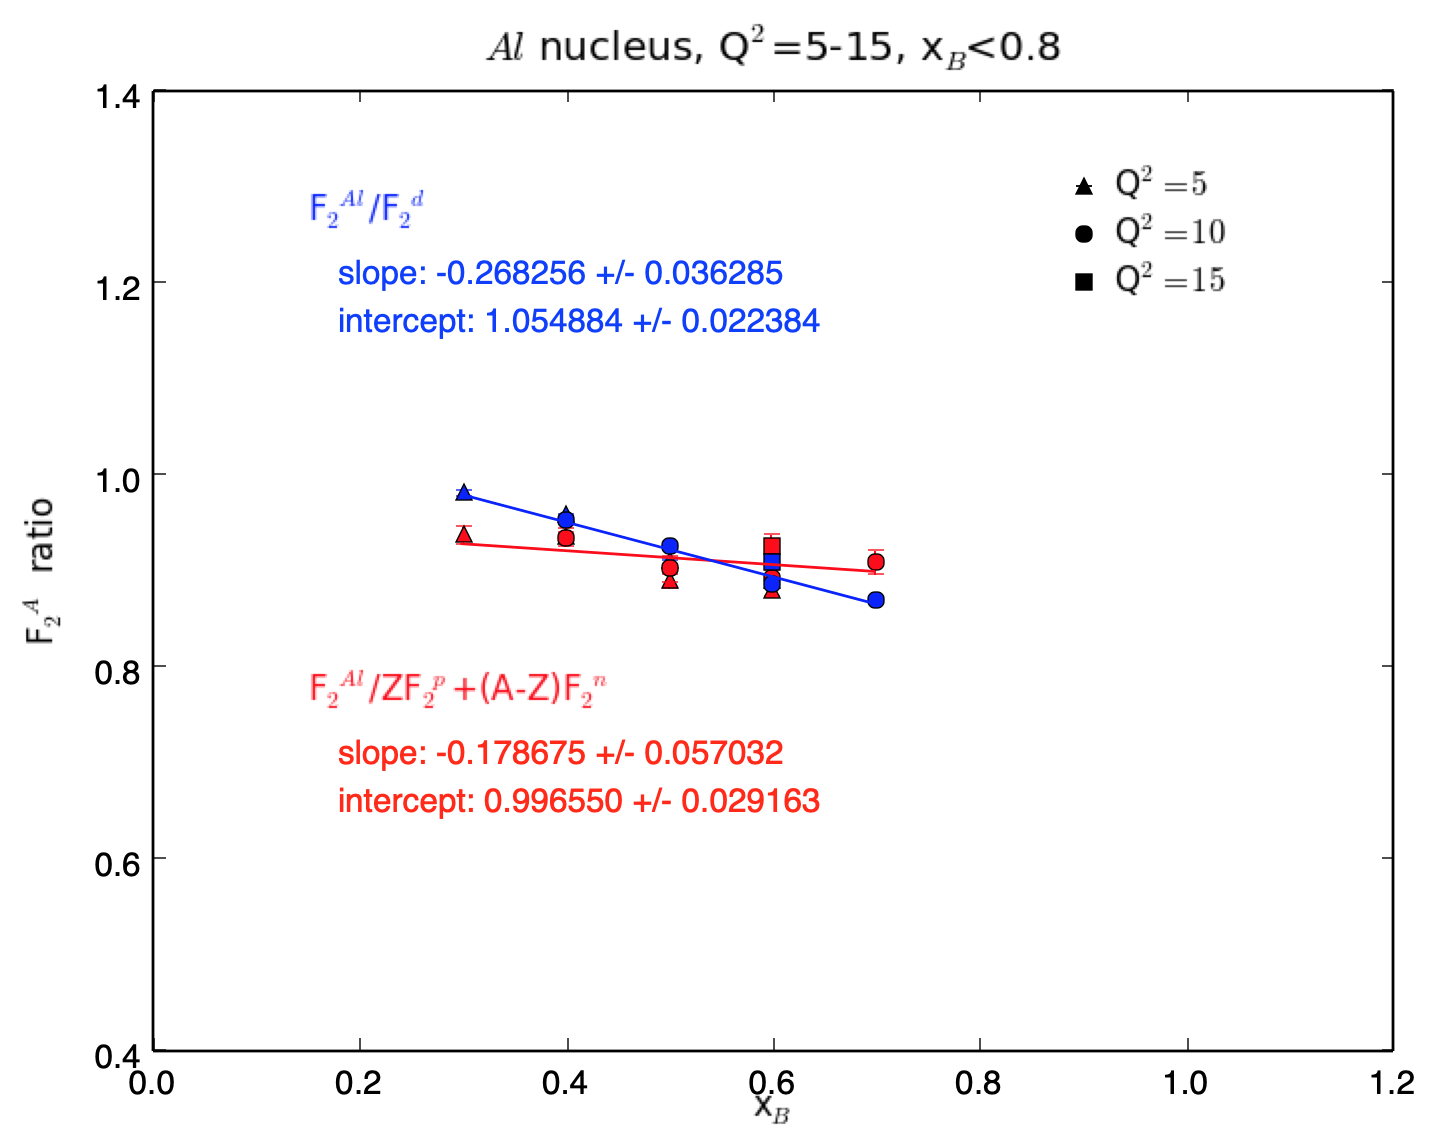
\includegraphics[width=\textwidth]{plots/q2_all_x_all/all_Al.png}
\end{minipage}
  \caption[]{Linear fits to the $Al$ target data with cuts on $Q^2$ and $x_B$.}
  \label{fig:fits_Al}
\end{figure}   


 \begin{figure}[H]
\begin{minipage}{0.5\textwidth}
 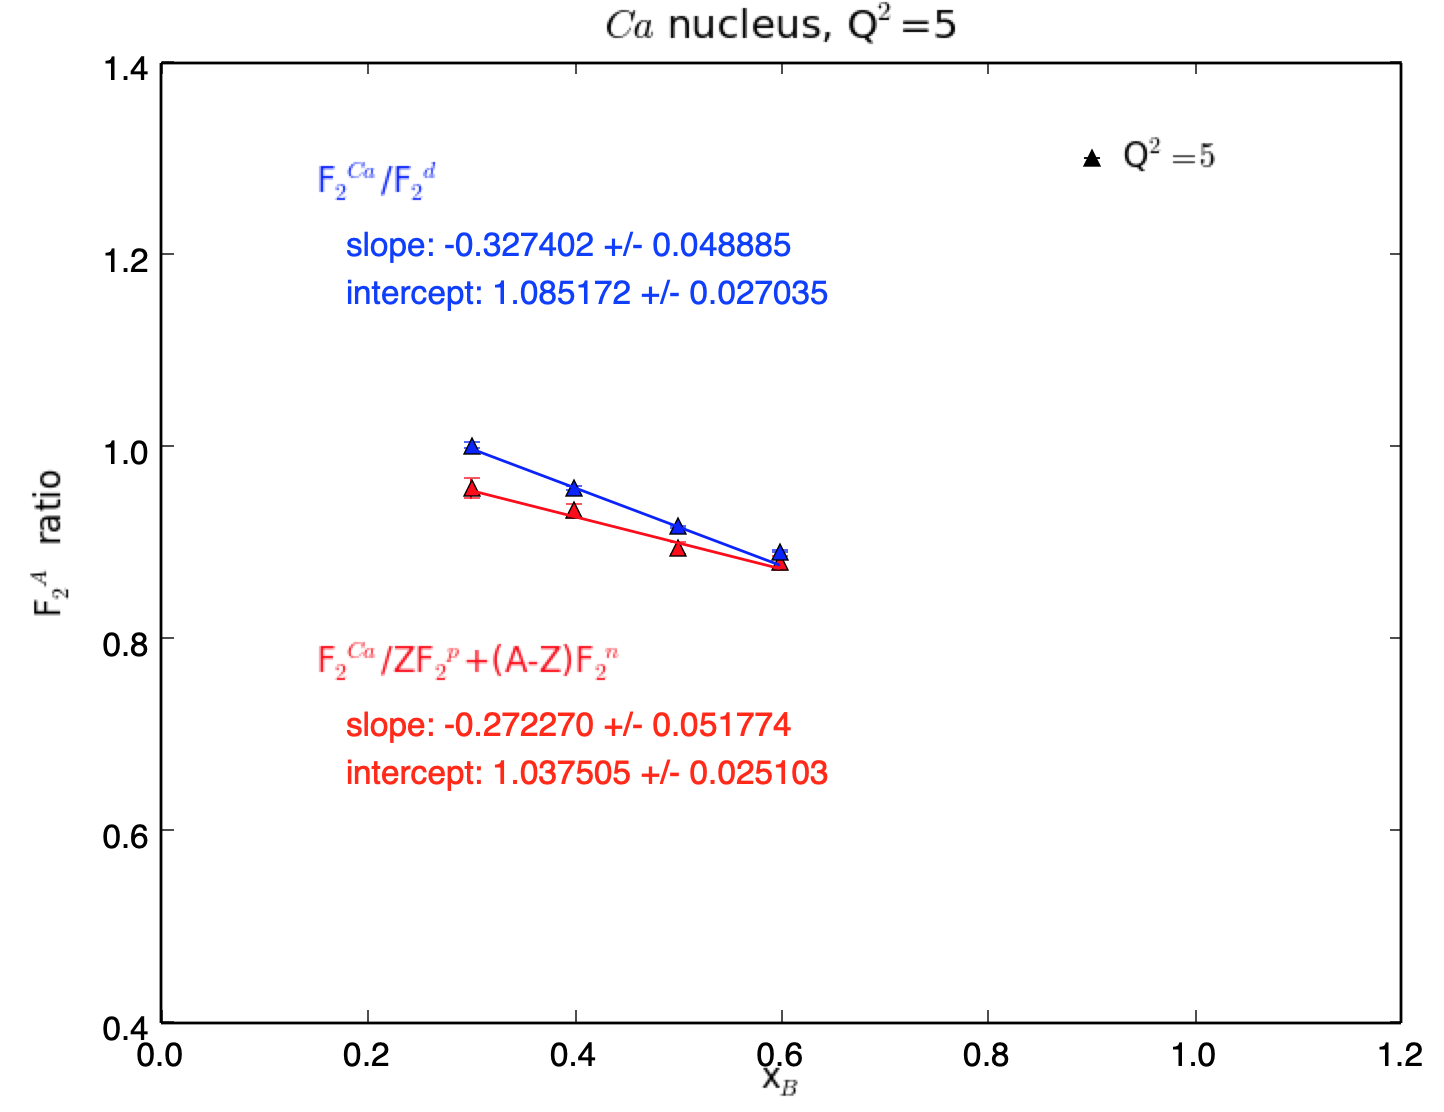
\includegraphics[width=\textwidth]{plots/q2_5/q2_5_Ca.png}
\end{minipage}\hfill\begin{minipage}{0.5\textwidth}
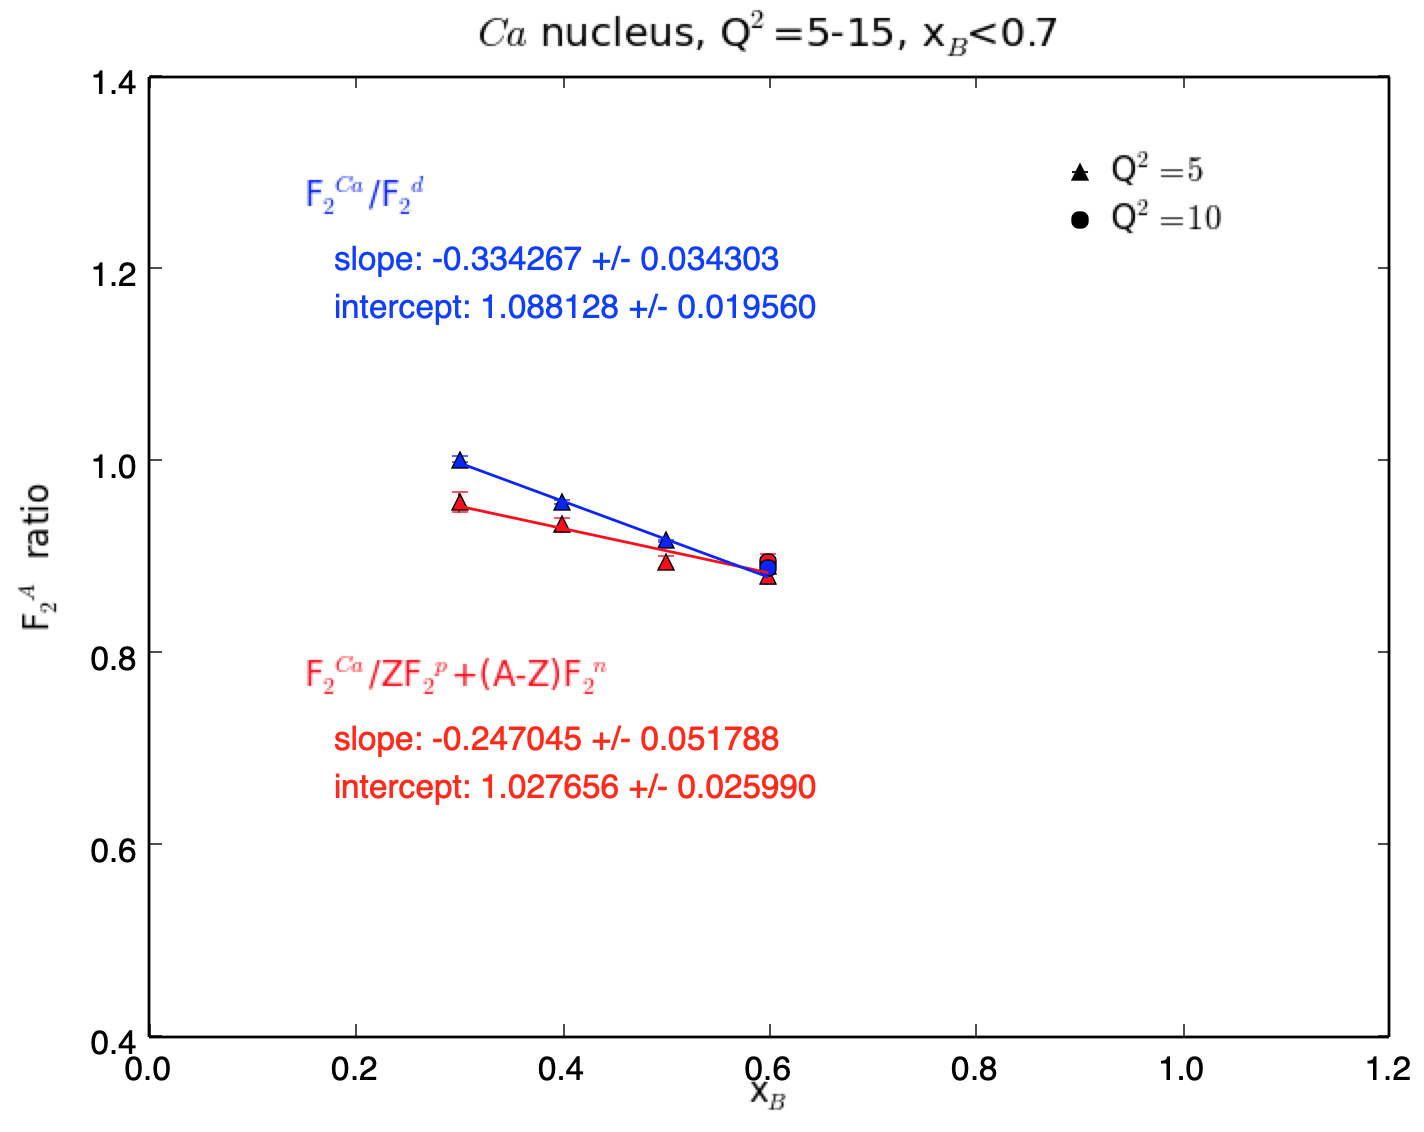
\includegraphics[width=\textwidth]{plots/q2_all_x_l7/q2_all_x_l7_Ca.png}
\end{minipage}\hfill\begin{minipage}{0.5\textwidth}
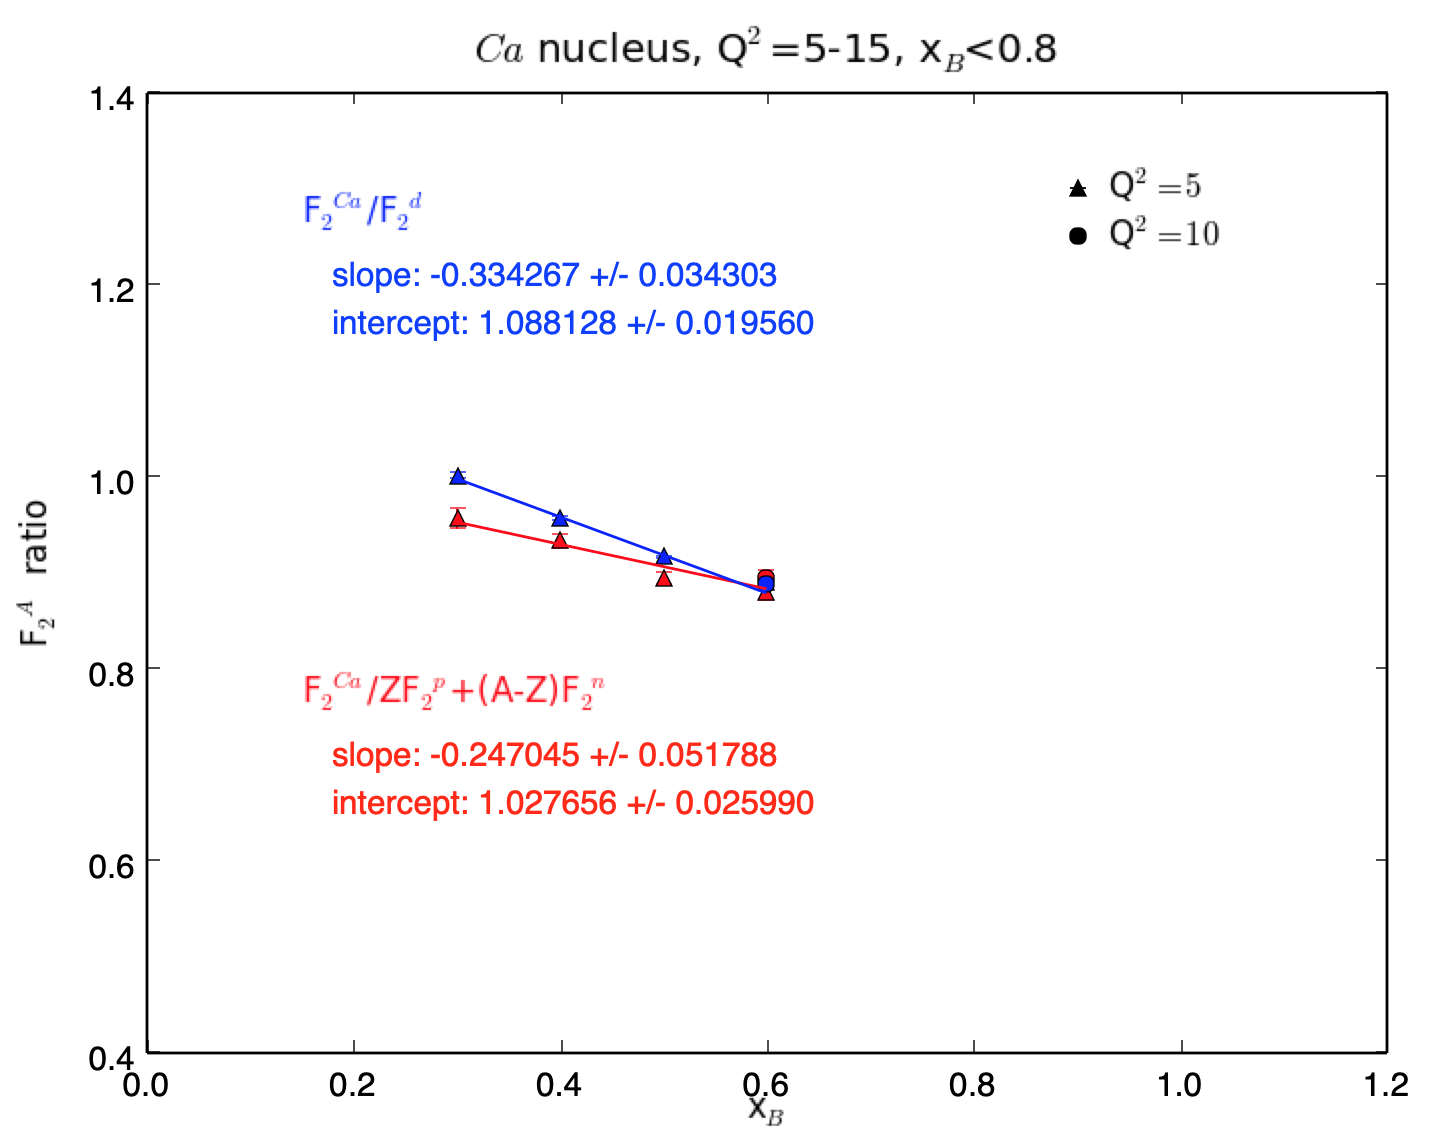
\includegraphics[width=\textwidth]{plots/q2_all_x_all/all_Ca.png}
\end{minipage}
  \caption[]{Linear fits to the $Ca$ target data with cuts on $Q^2$ and $x_B$.}
  \label{fig:fits_Ca}
\end{figure}   

 \begin{figure}[H]
\begin{minipage}{0.5\textwidth}
 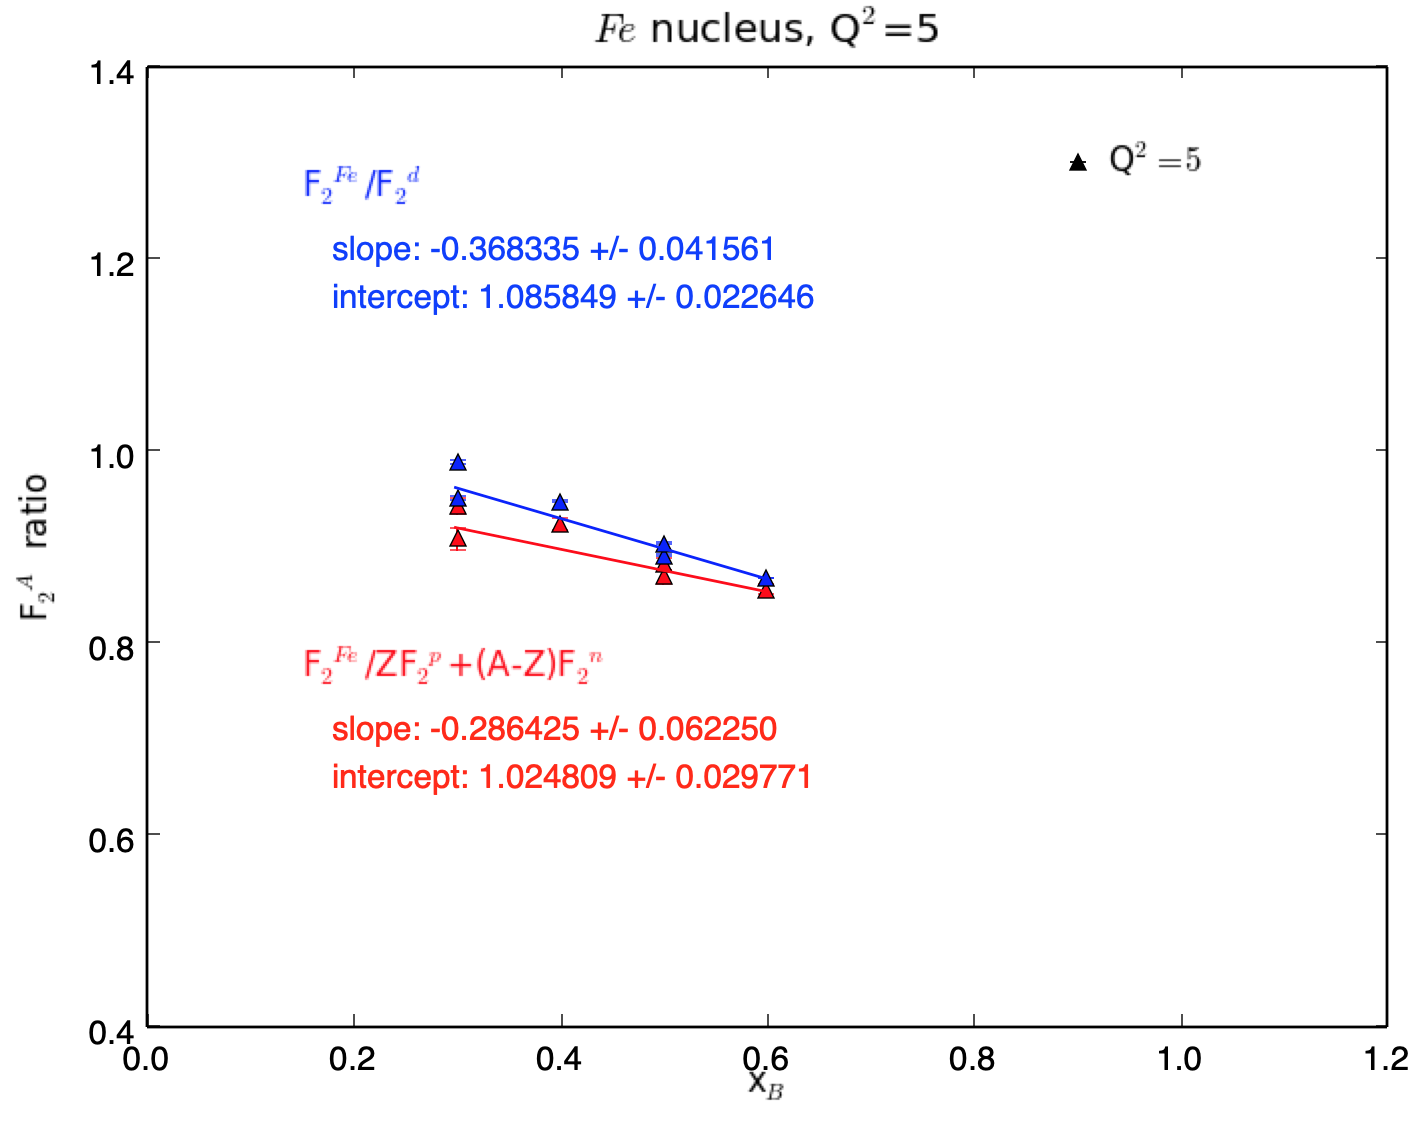
\includegraphics[width=\textwidth]{plots/q2_5/q2_5_Fe.png}
\end{minipage}\hfill\begin{minipage}{0.5\textwidth}
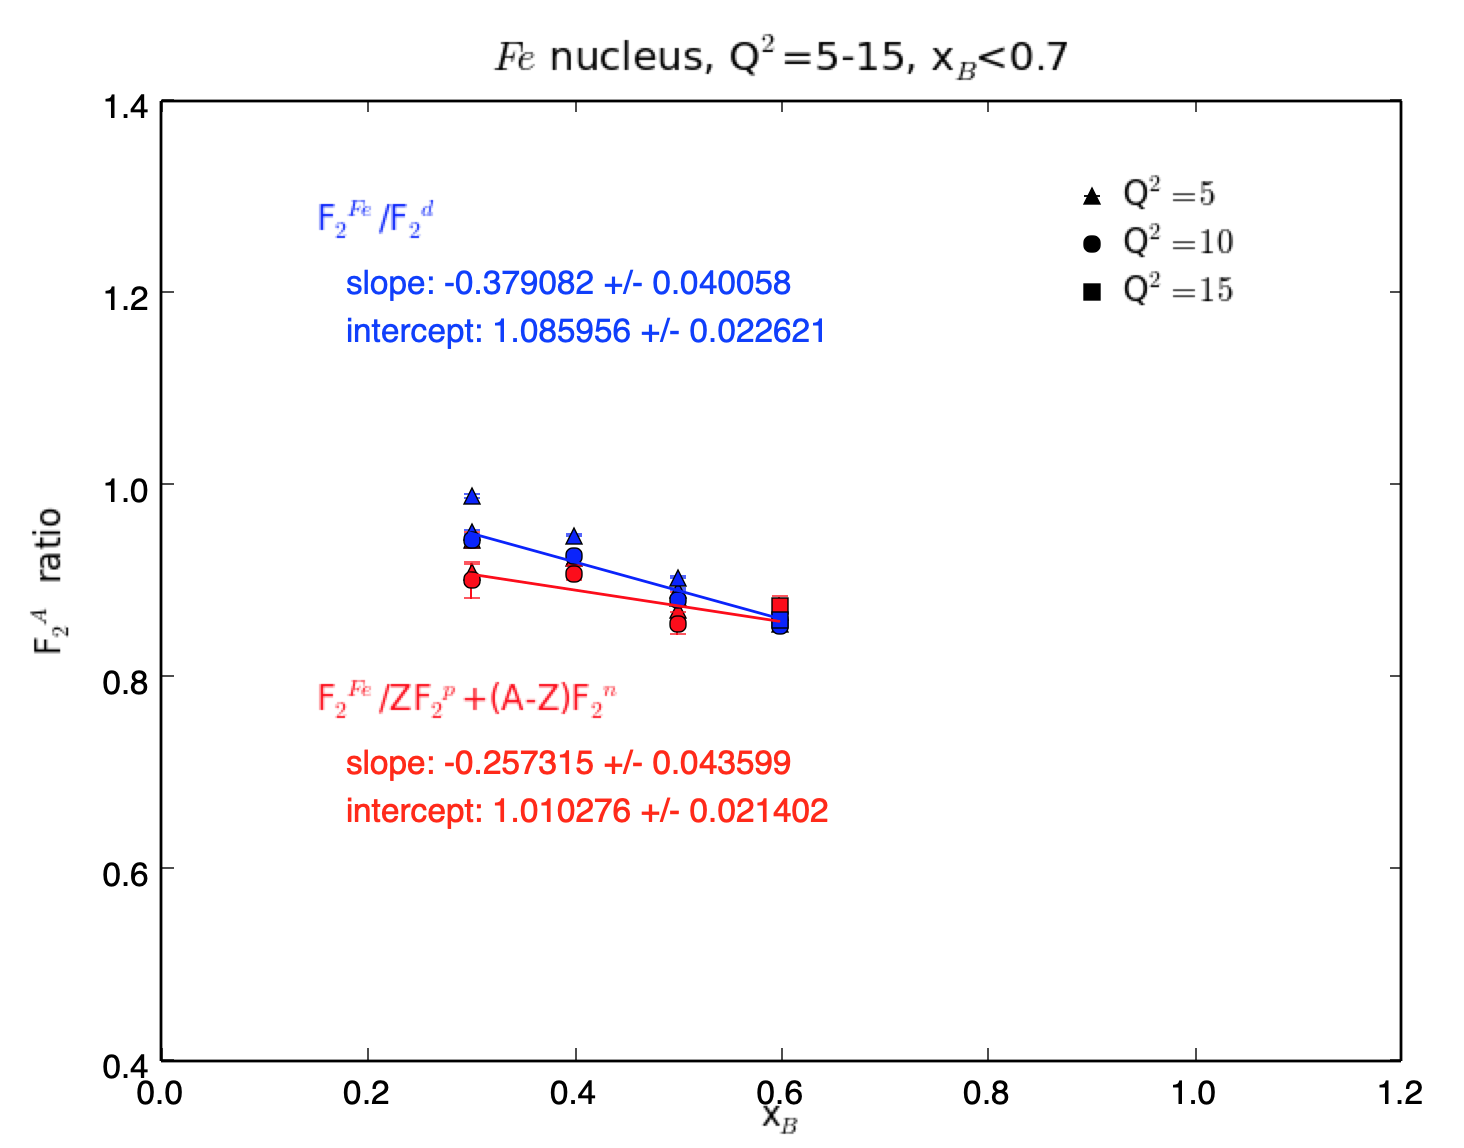
\includegraphics[width=\textwidth]{plots/q2_all_x_l7/q2_all_x_l7_Fe.png}
\end{minipage}\hfill\begin{minipage}{0.5\textwidth}
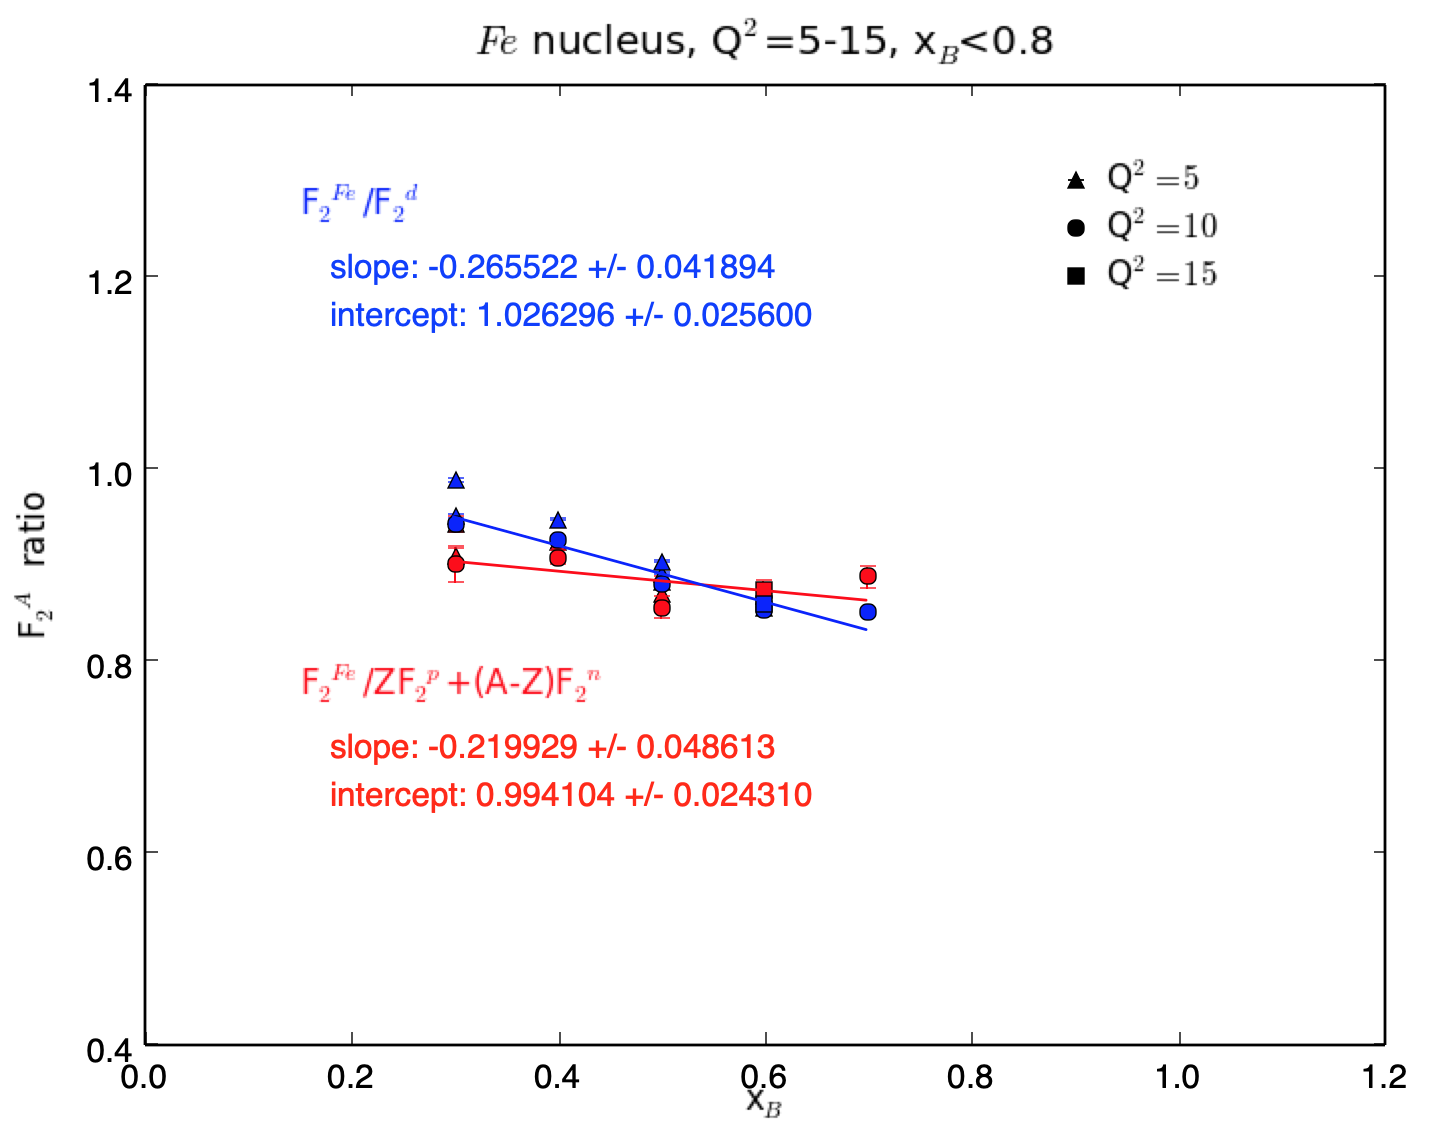
\includegraphics[width=\textwidth]{plots/q2_all_x_all/all_Fe.png}
\end{minipage}
  \caption[]{Linear fits to the $Fe$ target data with cuts on $Q^2$ and $x_B$.}
  \label{fig:fits_Fe}
\end{figure}   

 \begin{figure}[H]
\begin{minipage}{0.5\textwidth}
 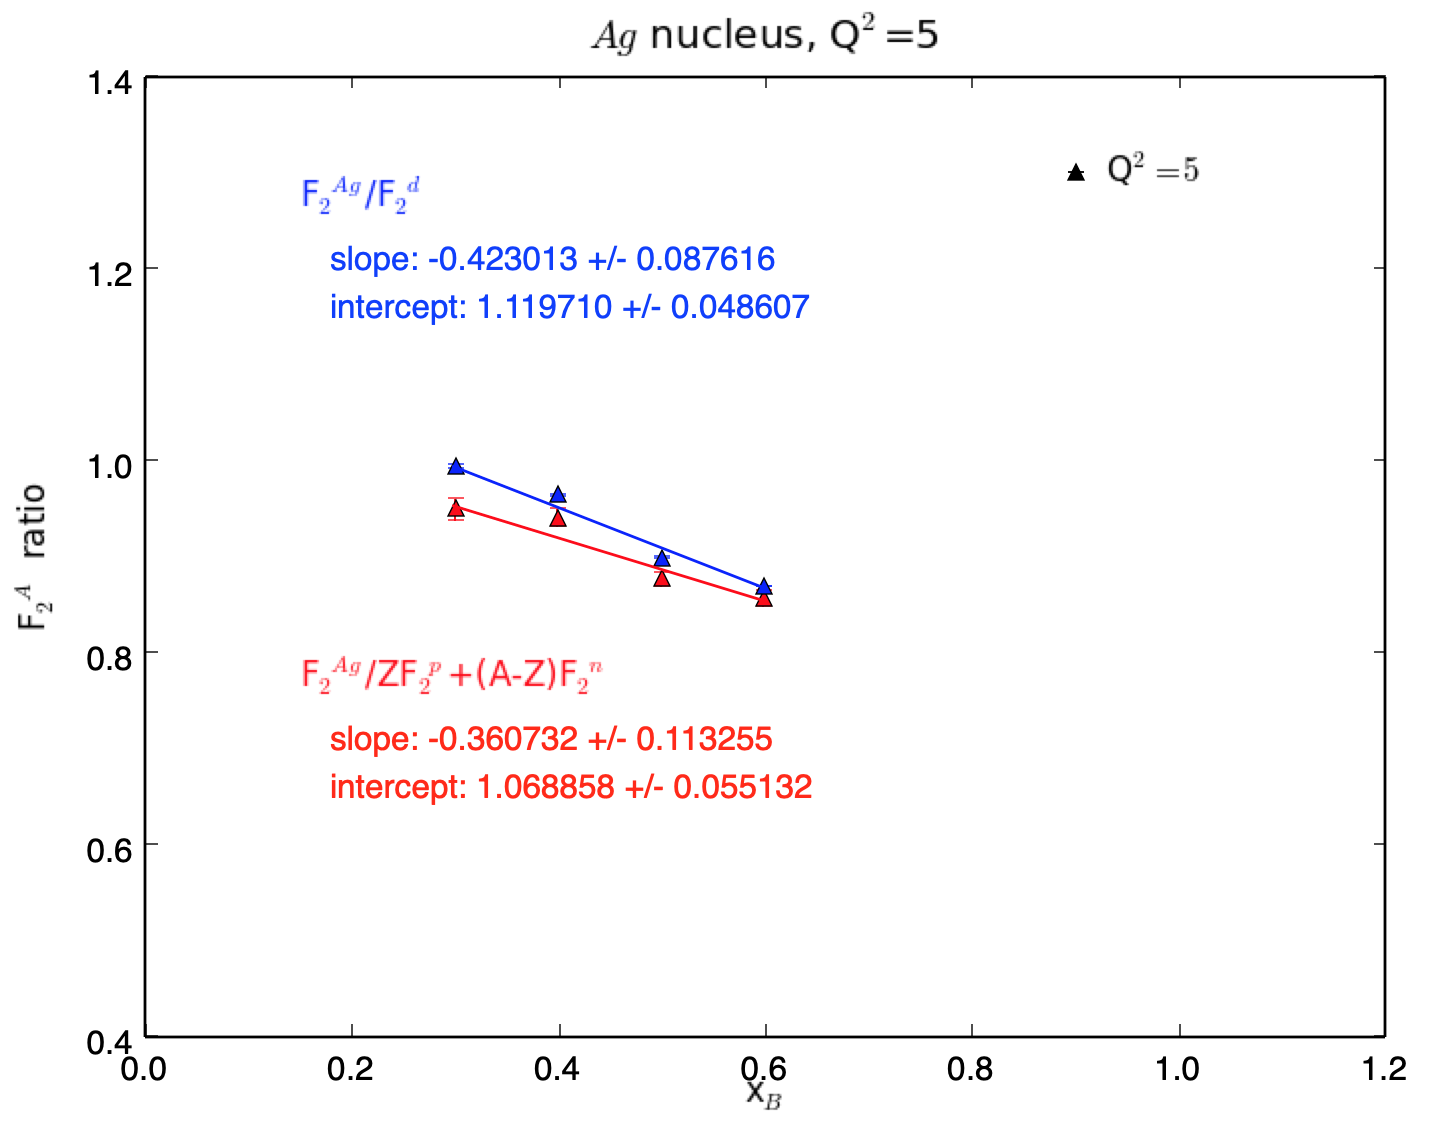
\includegraphics[width=\textwidth]{plots/q2_5/q2_5_Ag.png}
\end{minipage}\hfill\begin{minipage}{0.5\textwidth}
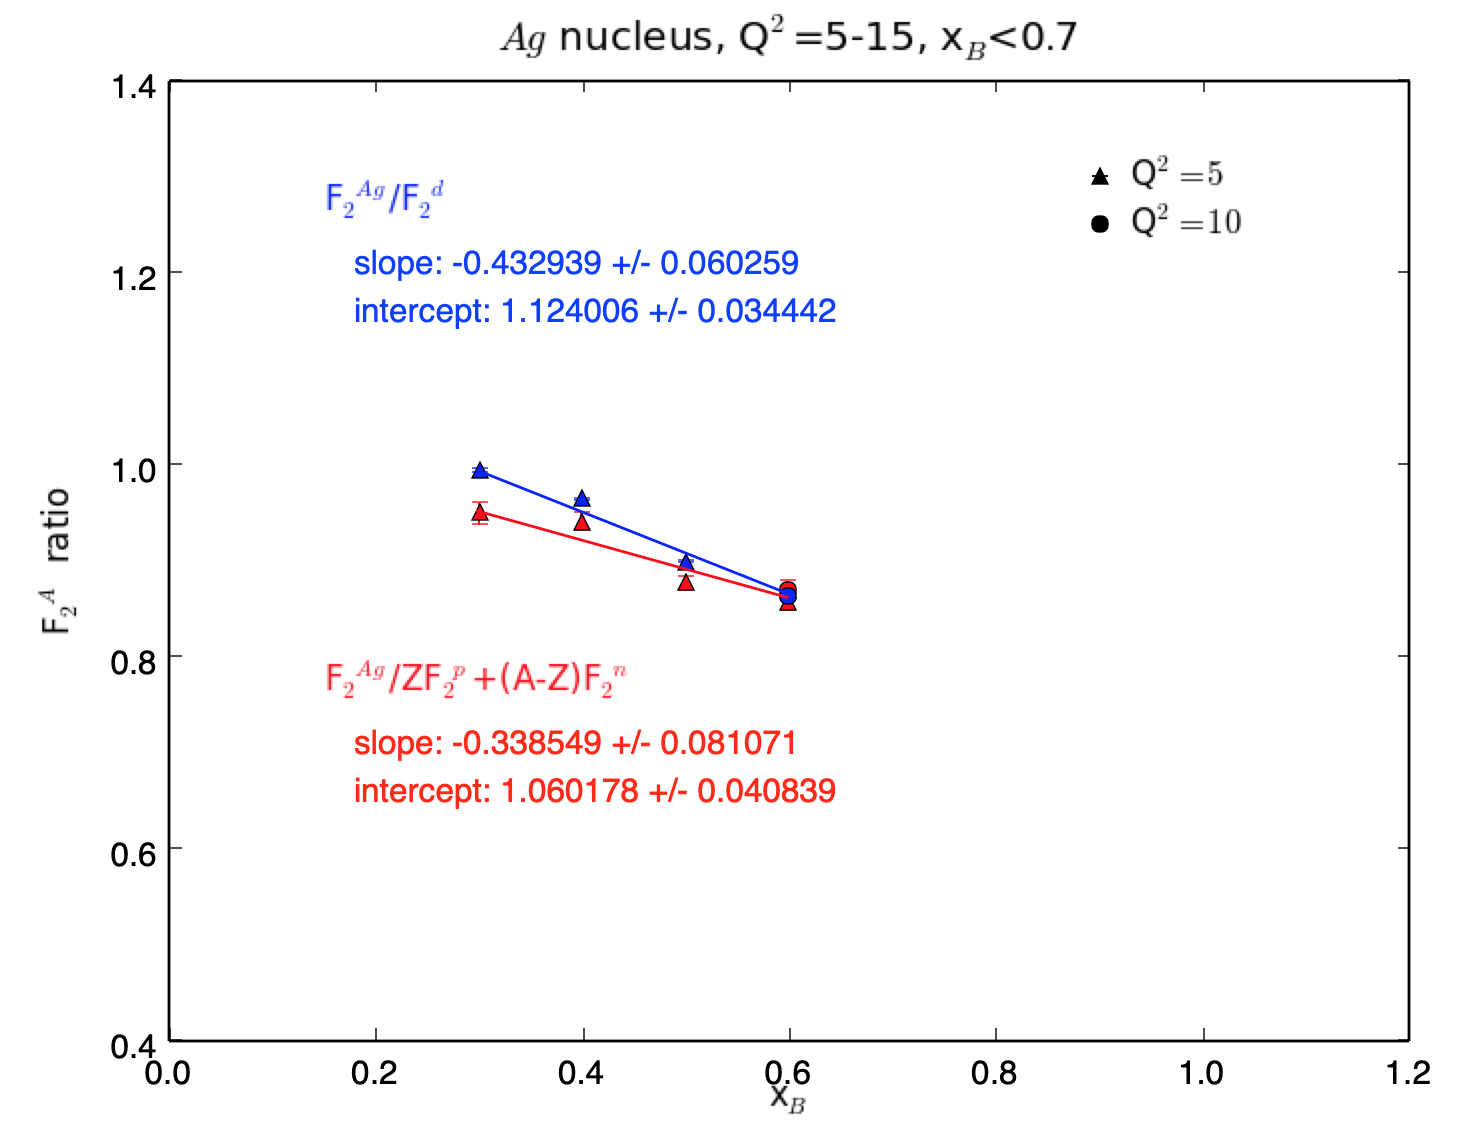
\includegraphics[width=\textwidth]{plots/q2_all_x_l7/q2_all_x_l7_Ag.png}
\end{minipage}\hfill\begin{minipage}{0.5\textwidth}
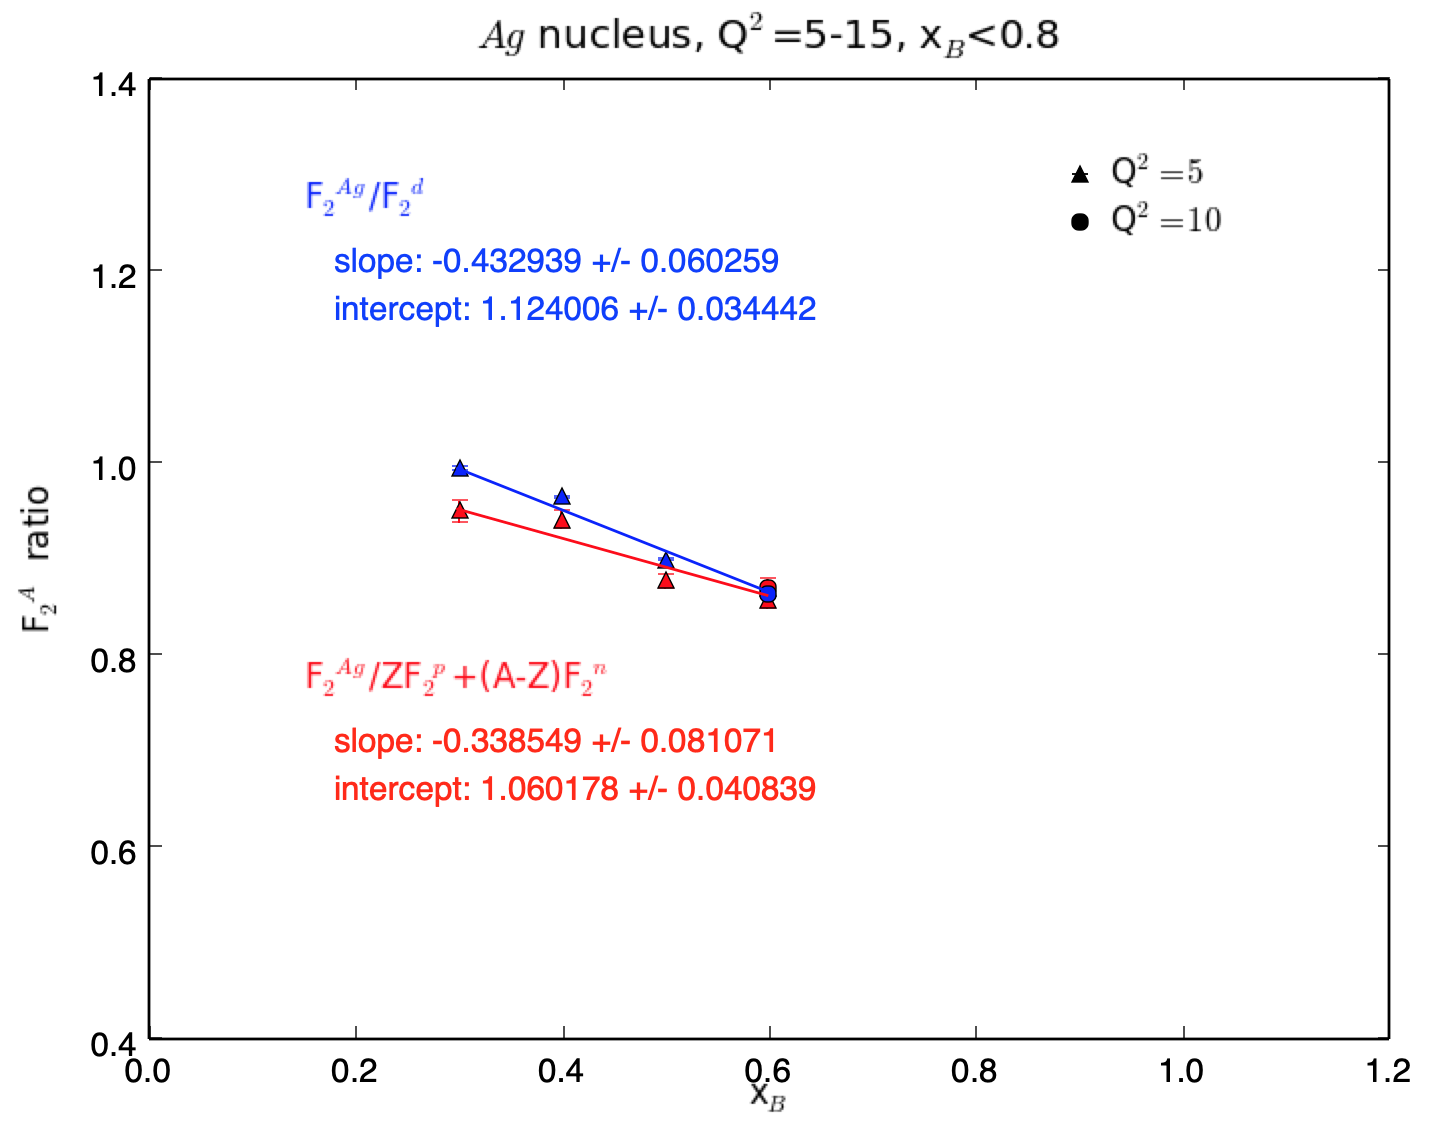
\includegraphics[width=\textwidth]{plots/q2_all_x_all/all_Ag.png}
\end{minipage}
  \caption[]{Linear fits to the $Ag$ target data with cuts on $Q^2$ and $x_B$.}
  \label{fig:fits_Ag}
\end{figure}   
 
\end{document}
